\chapter{Robust linear regression}
\label{chap:robreg}

This chapter is devoted to the estimation of the parameters of linear
regression models. Let us first precise some notations.

\section{The linear regression model}

In a linear regression model, we try to explain a variable $y$---the
\emph{dependent} variable---as a linear function of some \emph{explanatory}
variables (or \emph{predictors}) $x_{1}, \dots, x_{p}$: we assume that
%
\begin{equation}
    \label{eq:linear_regr_model}
    y = \beta_{0} + \beta_{1}x_{1} + \dots + \beta_{p}x_{p} + \varepsilon
\end{equation}
%
where $\beta_{0}, \beta_{1}, \dots, \beta_{p}$ are unknown regression
coefficients---$\beta_{0}$ is called the \emph{intercept} and $\beta_{1},
\dots, \beta_{p}$ are the \emph{slopes}---that have to be estimated and
$\varepsilon$ is a random error term (the error of the statistical model, due
to omitted factors, errors of measurement, random effects, etc.).

To estimate the regression coefficients, we need a random sample of
realizations of $(y_{i}, x_{i1}, \ldots, x_{ip})$, $i=1, \dots, n$, where $n$
is the sample size. We have
%
\begin{equation}
    \label{eq:linear_regr_model_sample}
    y_{i} = \beta_{0} + \beta_{1}x_{i1} + \dots + \beta_{p}x_{ip} + \varepsilon_{i},
    \qquad i = 1, \dots, n
\end{equation}
%
where $\varepsilon_{i}$'s are generally assumed to be i.i.d.\ random variables.
That is,
\[
    \varepsilon_{i} \stackrel{\text{i.i.d.}}{\sim} F_{0, \sigma}
\]
where distribution $F_{0, \sigma}$ has a location (centrality) parameter equal
to zero and a scale parameter equal to $\sigma$.

Denoting by $\stvec{x}_{i}$ and $\boldsymbol\beta$ the $(p+1)$ dimensional
column vectors with coordinates $(1, x_{i1}, \dots, x_{ip})$ and $(\beta_{0},
\beta_{1}, \dots, \beta_{p})$, respectively, equation
(\ref{eq:linear_regr_model_sample}) can be more compactly written as
%
\begin{equation}
    \label{eq:linear_regr_model_sample_bis}
    y_{i} = \stvec{x}_{i}'\boldsymbol\beta + \varepsilon_{i},
    \qquad i = 1, \dots, n, %
\end{equation}
%
Furthermore, letting $\stvec{y} = (y_{1}, \dots, y_{n})'$,
$\boldsymbol\varepsilon = (\varepsilon_{1}, \dots, \varepsilon_{n})'$ and
\[
    \stmat{X} = 
    \begin{bmatrix}
        1       & x_{11} & \dots & x_{1p} \\
        1       & x_{21} & \dots & x_{2p} \\
        \vdots  & \vdots & \dots & \vdots \\
        1       & x_{n1} & \dots & x_{np}
    \end{bmatrix}
    = 
    \begin{bmatrix}
        \stvec{x}_{1}' \\
        \stvec{x}_{2}' \\
        \vdots         \\
        \stvec{x}_{n}'
    \end{bmatrix}
\]
equations (\ref{eq:linear_regr_model_sample_bis}) takes the matrix-notation form
\[
    \stvec{y} = \stmat{X}\boldsymbol\beta + \boldsymbol\varepsilon
\]

Let us note here that, \emph{conditionally to the predictors}, the linear
regression model (\ref{eq:linear_regr_model_sample_bis}) may be considered as a
location-scale model. Indeed, under the assumption of homoscedasticity---an
identical scale parameter $\sigma$ for each error term
$\varepsilon_{i}$---regression model (\ref{eq:linear_regr_model_sample_bis})
may be formulated as follows:
%
\begin{equation}
    \label{eq:location_scale_regr_model}
    y_{i} = \stvec{x}_{i}'\boldsymbol\beta + \sigma\nu_{i}, 
    \qquad i = 1, \dots, n
\end{equation}
%
where the $\nu_{i}$'s are i.i.d.\ with distribution function $F_{0,1}$ (a
distribution with a location parameter equal to zero and a scale parameter
equal to one). In this case, the conditional distribution of $y_{i}$ given
$\stvec{x}_{i}$ is of the form:
%
\begin{equation}
    \label{eq:distr_function_yi}
    F_{y_{i} | \stvec{x}_{i}}(y) 
    = \Pr(y_{i} \leq y | \stvec{x}_{i}) 
    = \Pr\left(\nu_{i} \leq \frac{y - \stvec{x}_{i}'\boldsymbol\beta}{\sigma} \bigg| \stvec{x}_{i}\right)
    = F_{0,1}\left(\frac{y - \stvec{x}_{i}'\boldsymbol\beta}{\sigma}\right)
\end{equation}
%
Furthermore, if $f_{0,1}$ denotes the density function of the error terms 
$\nu_{i}$, that is,
\[
    f_{0,1}(u) = \frac{d F_{0,1}(u)}{d u} = F_{0,1}'(u)
\]
then
%
\begin{equation}
    \label{eq:dens_function_yi}
    f_{y_{i} | \stvec{x}_{i}}(y) 
    = \frac{1}{\sigma} f_{0,1}\left(\frac{y - \stvec{x}_{i}'\boldsymbol\beta}{\sigma}\right)
\end{equation}
%
Hence, $\stvec{x}_{i}'\boldsymbol\beta$ corresponds to the unknown location
parameter of the distribution of $y_{i}$ and $\sigma$ is the scale parameter of
the distribution of $y_{i}$. For simplicity, we will consider that the
distribution $F_{0,1}$ is continuous and symmetric around zero (and exception
is Section \ref{sec:inference}).

\begin{stremark}
The classic \emph{location-scale model} may be seen as a particular case of
regression model (\ref{eq:location_scale_regr_model}). It suffices to set
$\beta_{1} = \dots = \beta_{p} = 0$ and to assume that the $\nu_{i}$'s are
i.i.d.\ with distribution $F_{0,1}$ (such that $E(\nu_{i})=0$). In this case,
the observations
%
\begin{equation}
    \label{eq:location_scale_model}
    y_{i} = \beta_{0} + \sigma\nu_{i},
    \qquad i=1, \dots, n,
\end{equation}
%
are i.i.d.\ with a common distribution $F$ characterized by mean $\mu =
\beta_{0}$ and scale parameter $\sigma$.
\end{stremark}

\begin{stremark}
Most textbook presentations of the linear regression model assume the
explanatory variables to be fixed (and measured without error). That is, the
explanatory variables are not assumed to be random variables. In the context of
a \emph{designed experiment}, this assumption is reasonable since the values of
the experimental factors are determined \emph{a priori} by the researchers. In
other contexts such as, for example, when using social-science survey data, the
assumption makes no sense. \alert{[Say here what the consequence is: The fact
that the $X$'s are random doesn't really change anything. (unlike measurement
error which attenuates the estimates)]}

Nonetheless, since we focus on the problem of outlying values, we will ignore
the issue in this chapter and consider $x_{ij}$, $i = 1, \dots, n$, $j = 1,
\dots, p$, as predetermined. That is, results will always be conditional on the
particular \emph{values} taken by the explanatory variables.

\alert{I'm not sure whether this remark makes sense. First, LS results are
valid also if the $X$'s are random. Second, if we talk about $X$ outliers it
makes not much sense to assume $X$ fixed.}
\end{stremark}


\section{Different types of outliers}

Model (\ref{eq:linear_regr_model}) assume that \emph{all} units of the
population and, \emph{de facto}, all units of the sample are consistent with
the supposed linear model. If a unit has a behavior that does not respect the
underlying theoretical model, we define it as an \emph{outlying} unit with
respect to the model.

Of course, in the case of \emph{simple} linear regression model ($p=1$), a
visual inspection of the scatterplot is generally sufficient to detect the
outliers. But, when the number of explanatory variables is greater than two,
it becomes impossible to visualize all the data set and the use of robust
methods to estimate the regression parameters is then essential. More
precisely, we aim at developing procedures that provide a good fit to the bulk
of the data without being perturbed by a small proportion of outliers, and
that do not require deciding previously which observations are outliers.
Moreover, the comparison between the estimations provided by the classical
least squares estimator and those obtained using a robust estimation procedure
will allow to bring to the fore the outlyingness of some data.

In cross-sectional regression analysis, three types of outliers may influence
the estimations. \citet{rousseeuw:leroy:1987} define them as \emph{vertical
outliers}, \emph{good leverage points} and \emph{bad leverage points}. To
illustrate this terminology, consider a simple linear regression as shown in
figure~\ref{fig:outlier_types} (the generalization to higher dimensions is
straightforward). \emph{Vertical outliers} are those observations that have
outlying values for the corresponding error term (that is, in the
$y$-dimension) but are not outlying in the space of explanatory variables (in
the $x$-dimension). \emph{Good leverage points} are observations that are
outlying in the space of explanatory variables but that are located close to
the regression hyperplane. Finally, \emph{bad leverage points} are observations
that are both outlying in the space of explanatory variables and located far
from the true regression hyperplane.


\begin{figure}[h!]
    \centering
    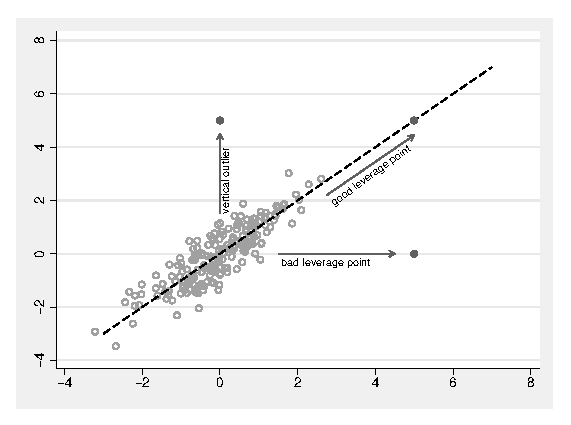
\epsfig{file=eps/4/1}
    \caption{Vertical outlier, good leverage point and bad leverage point}
    \label{fig:outlier_types}
\end{figure}

All these types of outliers risk to affect the estimation of the regression
hyperplane but their effect changes according to the estimator we will
consider and the type of outlyingness. For the classical least squares
estimation method, for instance, the bad leverage points are considered as the
most dangerous outliers because their presence can change the sign of the
slope of the regression line (in simple regression); the good leverage points
have little influence on the estimation of the regression coefficients but
they have an impact on the variances and covariances of the regression
coefficients' estimators and, consequently, risk to influence the inferential
procedures (tests and confidence intervals).

The most popular estimation method in linear regression is certainly the
\emph{least squares} (\stsc{LS}) method introduced in 1805 by Legendre
\alert{[Citation?]}. One of its principal advantage is the simplicity of the
computation of the \stsc{LS} estimates. Its popularity has also be reinforced
by the fact that, under the normality of the error terms, \stsc{LS} estimates
of the regression coefficients coincide with the maximum likelihood estimates.
We will first briefly review the logic behind least squares (\stsc{LS})
estimation and recall why the \stsc{LS} estimator is particularly affected by
the presence of atypical individuals. We will thereafter introduce some
alternative estimation methods that have been proposed to try to cope with
outliers.


\section{LS estimation}

Let us denote by $\sthat{y}_{i}(\boldsymbol\beta)$ the value fitted by the
regression model for the $i$th statistical unit of the sample when taking
$\boldsymbol\beta$ as value for the vector of regression coefficients:
\[
    \sthat{y}_{i}(\boldsymbol\beta)  = \stvec{x}_{i}'\boldsymbol\beta, 
    \qquad i = 1, \dots, n
\]
The difference between the observed value $y_{i}$ and the fitted value
$\sthat{y}_{i}(\boldsymbol\beta)$ is the residual $r_{i}(\boldsymbol\beta)$:
\[
    r_{i}(\boldsymbol\beta) = y_{i} - \sthat{y}_{i}(\boldsymbol\beta),
    \qquad i = 1, \dots, n
\]

Although $\boldsymbol\beta$ can be estimated in several ways, the underlying
idea is often to take an estimate $\sthat{\boldsymbol\beta}$ in such a way that
the fitted values $\sthat{y}_{i}(\sthat{\boldsymbol\beta})$ for the dependent
variable are as close as possible to the observed values $y_{i}$ ($i = 1,
\dots, n$), i.e., in such a way that we minimize globally the magnitude of the
residuals $r_{i}(\sthat{\boldsymbol\beta})$. This idea leads to try to find the
estimate $\sthat{\boldsymbol\beta}$ that minimizes a specific aggregate
prediction error.

In the case of the well-known ordinary least squares (\stsc{LS}), this
aggregate prediction error is defined as the sum of squared residuals:
%
\begin{equation}\label{eq:LS_min}
    \sthat{\boldsymbol\beta}_{\stsc{LS}} = \arg\min_{\boldsymbol\beta} 
    \sum_{i=1}^{n} r_{i}^{2}(\boldsymbol\beta)
\end{equation}
%
where “$\arg\min$” stands for “the value minimizing”. In other terms,
$\sthat{\boldsymbol\beta}_{\stsc{LS}}$ is solution of the so called
\emph{normal equations} system --- we will also call it the \emph{estimating
equations} system --- obtained by differentiating the function $\sum_{i=1}^{n}
r_{i}^{2}(\boldsymbol\beta)$ to minimize with respect to each component of
$\boldsymbol\beta$, that is, $\sthat{\boldsymbol\beta}_{\stsc{LS}}$ is the
solution of
%
\begin{equation}\label{eq:LS_equations}
    \sum_{i=1}^{n}  r_{i}(\boldsymbol\beta)\stvec{x}_{i} = \stvec{0}
\end{equation}
%
which is equivalent to the linear equations system
\[
    \stmat{X}'\stmat{X}\boldsymbol\beta = \stmat{X}'\stvec{y}.
\]
If $\stmat{X}$ has full rank\footnote{The matrix of predictors $\stmat{X}$ is
said to have \emph{full rank} if its columns are linearly independent (absence
of multicollinearity), that is, if $\stmat{X}\stvec{a}\neq\stvec{0}$ for all
$\stvec{a}\neq\stvec{0}$. This is equivalent to the nonsingularity of
$\stmat{X}'\stmat{X}$.}, then the solution of (\ref{eq:LS_equations}) is unique
and is given by
%
\begin{equation}\label{eq:LS_estimator}
    \sthat{\boldsymbol\beta}_{\stsc{LS}}
    = \sthat{\boldsymbol\beta}_{\stsc{LS}}(\stmat{X}, \stvec{y})
    = (\stmat{X}'\stmat{X})^{-1} \stmat{X}'\stvec{y}
\end{equation}
%
This estimate can be computed in Stata using the \stcmd{regress} command (see
\rref{regress}).

Note here that, if the model contains a constant term $\beta_{0}$, that is, if
the first component of the vectors $\stvec{x}_{i}$, $i = 1, \dots, n$, is equal
to one, it follows from (\ref{eq:LS_equations}) that the residuals
$r_{i}(\sthat{\boldsymbol\beta}_{\stsc{LS}})$, $i = 1, \dots, n$, have zero
average.

It is easy to verify that the \stsc{LS} estimator satisfies 
(see \citealp[92]{maronna:etal:2006})
%
\begin{align}
    \label{eq:regression_equivariance}
    \sthat{\boldsymbol\beta}_{\stsc{LS}}(\stmat{X},\stvec{y}+\mathbf{X}\boldsymbol\gamma) 
        &= \sthat{\boldsymbol\beta}_{\stsc{LS}}(\stmat{X},\stvec{y})+\boldsymbol\gamma
        \qquad\text{for all $\boldsymbol\gamma\in\mathbb{R}^{p+1}$} \\
    \label{eq:scale_equivariance}
    \sthat{\boldsymbol\beta}_{\stsc{LS}}(\stmat{X},\lambda\stvec{y})
        &= \lambda\sthat{\boldsymbol\beta}_{\stsc{LS}}(\stmat{X}, \stvec{y})
        \qquad\text{for all $\lambda\in\mathbb{R}$}
\end{align}
%
and, for any nonsingular $(p+1) \times (p+1)$ matrix $\stmat{A}$,
%
\begin{equation}\label{eq:affine_equivariance}
    \sthat{\boldsymbol\beta}_{\stsc{LS}}(\stmat{X}\stmat{A},\stvec{y})
    = \stmat{A}^{-1}\sthat{\boldsymbol\beta}_{\stsc{LS}}(\stmat{X},\stvec{y})
\end{equation}
%
The properties (\ref{eq:regression_equivariance}),
(\ref{eq:scale_equivariance}) and (\ref{eq:affine_equivariance}) are called
\emph{regression}, \emph{scale} and \emph{affine equivariance} of
$\sthat{\boldsymbol\beta}_{\stsc{LS}}$, respectively. In the sequence, it will
be desirable that every other estimator of $\boldsymbol\beta$ also satisfies
these natural properties.

It is also well known that the \stsc{LS} estimator of $\boldsymbol\beta$ coincides
with the maximum likelihood estimator in case of normally distributed error
terms in (\ref{eq:linear_regr_model_sample}). Hence, $\widehat
{\boldsymbol\beta}_{\stsc{LS}}$ is the most efficient estimator of
$\boldsymbol\beta$ in the Gaussian regression model.

However, an important drawback of \stsc{LS} is that, by considering squared
residuals, it tends to award an excessive importance to observations with large
residuals and, consequently, distort parameters estimation when outliers exist.

\section{M estimation}

\subsection{L\textsubscript{1} or Least Absolute Deviation (LAD) estimation}

\citet{edgeworth:1887} realized that due to the squaring of the residuals,
\stsc{LS} becomes extremely vulnerable to the presence of outliers. To cope
with this, he proposed a method consisting in minimizing the sum of the
absolute values of the residuals rather than the sum of their squares. More
precisely, his method defines the $L_{1}$ or \emph{least absolute deviation}
(\stsc{LAD}) estimate as
%
\begin{equation}\label{eq:L1_min}
    \sthat{\boldsymbol\beta}_{\stsc{LAD}} 
        = \arg\min_{\boldsymbol\beta} \sum_{i=1}^{n} |r_{i}(\boldsymbol\beta)|
\end{equation}
%
This estimate is solution of the estimating equations system obtained by
differentiating the sum of the absolute values of the residuals with respect
to each component of $\boldsymbol\beta$:
%
\begin{equation}\label{eq:L1_equations}
    \sum_{i=1}^{n}\sign(r_{i}(\sthat{\boldsymbol\beta}_{\stsc{LAD}})) 
    \stvec{x}_{i} = \stvec{0}
\end{equation}
%
If the model contains an intercept term, (\ref{eq:L1_equations}) implies that
the residuals $r_{i}(\sthat{\boldsymbol\beta}_{\stsc{LAD}})$, $i = 1, \dots,
n$, have a median equal to zero; this motivates the fact that the \stsc{LAD}
regression estimator is also sometimes called the \emph{median regression
estimator}.

Unlike for $\sthat{\boldsymbol\beta}_{\stsc{LS}}$, there is no explicit
expression for $\sthat{\boldsymbol\beta}_{\stsc{LAD}}$.\footnote{Note also that
the \stsc{LAD} estimate of $\boldsymbol\beta$ may not be unique and has the
property that at least $(p+1)$ residuals are equal to zero.} However, there
exist very fast algorithms to compute it and
$\sthat{\boldsymbol{\beta}}_{\stsc{LAD}}$ is available in Stata via the
\stcmd{qreg} command as a standard function (see \rref{qreg}).

Finally, it can easily be seen from (\ref{eq:L1_min}) and
(\ref{eq:L1_equations}) that this estimator does protect against vertical
outliers (but not against bad leverage points). However, this gain in
robustness with respect to the \stsc{LS} estimator comes with an important loss
of efficiency: the asymptotic relative efficiency of
$\sthat{\boldsymbol{\beta}}_{\stsc{LAD}}$ with respect to
$\sthat{\boldsymbol\beta}_{\stsc{LS}}$ is equal to $2/\pi = 63.7\%$ at a
Gaussian error distribution (see \citealp{huber:1981}).

\subsection{The principle of M estimation}

\citet{huber64} hence generalized median regression to a wider class of
estimators, called \stsc{M} estimators, by considering other functions than
the absolute value in (\ref{eq:L1_min}) in order to find a reasonable balance
between robustness and Gaussian efficiency.

An \stsc{M} estimate $\sthat{\boldsymbol\beta}_{\stsc{M};\rho}$ of
$\boldsymbol\beta$ is defined by
%
\begin{equation}
    \label{eq:M_min}
    \sthat{\boldsymbol\beta}_{\stsc{M};\rho} 
        = \arg\min_{\boldsymbol\beta}\sum_{i=1}^{n} 
            \rho\left(\frac{y_{i} - \stvec{x}_{i}'\boldsymbol\beta}{\sthat{\sigma}}\right)
        = \arg\min_{\boldsymbol\beta}\sum_{i=1}^{n}
            \rho\left(\frac{r_{i}(\boldsymbol\beta)}{\sthat{\sigma}}\right)
\end{equation}
%
where $\rho(u)$ is a loss function that is positive, even such that $\rho(0) =
0$, and non decreasing for positive values $u$, and $\sthat{\sigma}$ is an
auxiliary estimate of the scale parameter $\sigma$ required to standardize the
residuals and to make $\sthat{\boldsymbol\beta}_{\stsc{M};\rho}$ scale
equivariant; see (\ref{eq:scale_equivariance}). In most situations,
$\sthat{\sigma}$ is computed in advance, but it can also be computed
simultaneously through a scale \stsc{M} estimating equation. This problem will
be discussed in more details later.

\begin{stremark}
The \stsc{LS} estimate and the \stsc{LAD} estimate correspond respectively to
$\rho(u) = u^{2}$ and $\rho(u) = |u|$. In these two cases, $\sthat{\sigma}$
becomes a constant factor outside the summation sign in (\ref{eq:M_min}) and
\[
    \arg\min_{\boldsymbol\beta} \sum_{i=1}^{n} \rho\left(\frac{r_{i}(\boldsymbol\beta)}{\sthat{\sigma}}\right)
    = \arg\min_{\boldsymbol\beta}\sum_{i=1}^{n}\rho(r_{i}(\boldsymbol\beta))
\]
Thus neither the \stsc{LS} nor the \stsc{LAD} estimate require an auxiliary
scale estimate.
\end{stremark}

Of course, if we want a \stsc{M} estimator more robust against vertical
outliers than the \stsc{LS} estimator, we have to take a loss function $\rho$
that is less rapidly increasing than the square function in order to give less
weight to big (in absolute value) residuals in the minimization problem. In
order to combine robustness and efficiency under a Gaussian error distribution,
\citet{huber64} has suggested to use for $\rho$ a function of the form (see
figure~\ref{fig:rho_psi_Huber}):
\[
    \rho_{\kappa}^{\stsc{H}}(u) = 
    \begin{cases}
        u^{2}                    & \text{if $|u| \leq \kappa$}\\
        2\kappa |u| - \kappa^{2} & \text{if $|u| > \kappa$}
    \end{cases}
\]
where $\kappa$ is a constant determining the trade-off between robustness and
efficiency. These functions of Huber are convex on the whole real line and may
be seen as intermediate functions between the quadratic function (leading to
the non robust but efficient \stsc{LS} estimate) and the absolute value function
(associated with the robust but poorly efficient \stsc{LAD} estimate).

Another class of loss functions $\rho$ widely used in the literature is the
class of the Tukey-Biweight \alert{[Citation?]} functions (see figure~\ref{fig:rho_psi_Biweight})
%
\begin{equation}
    \label{eq:Tukey_Biweight_function}
    \rho_{\kappa}^{\stsc{B}}(u) = 
        \begin{cases}
            \frac{\kappa^{2}}{6} \left[1 - \left(1 - \left(\frac{u}{\kappa}\right)^{2}\right)^{3}\right] 
                & \text{if $|u| \leq \kappa$}\\
            \frac{\kappa^{2}}{6} 
                & \text{if $|u| > \kappa$}
        \end{cases}
\end{equation}
%
These functions are bounded. Once again, the constant $\kappa$ allows the
trade-off between robustness and Gaussian efficiency. We will show the
advantage and disadvantage to use a bounded function $\rho$ hereafter.

We may also characterize $\sthat{\boldsymbol\beta}_{\stsc{M};\rho}$ as a
solution of the estimating equations system obtained by differentiating the
function to minimize in (\ref{eq:M_min}) with respect to each component of
$\boldsymbol\beta$, that is, as a solution of the equations system
%
\begin{equation}\label{eq:M_equations}
    \sum_{i=1}^{n} \psi\left(\frac{r_{i}(\boldsymbol\beta)}{\sthat{\sigma}}\right) \stvec{x}_{i} = \stvec{0}
\end{equation}
%
where $\psi(u) = d\rho(u) / du = \rho'(u)$. For instance, taking
$\rho(u)=\rho_{\kappa}^{\stsc{H}}(u)$, we have
\[
    \psi_{\kappa}^{\stsc{H}}(u) = 
    \begin{cases}
        -2\kappa    & \text{if $u<-\kappa$}\\
        2u          & \text{if $-\kappa\leq u\leq\kappa$}\\
        2\kappa     & \text{if $u>\kappa$}
    \end{cases}
\]
for $\rho(u) = \rho_{\kappa}^{\stsc{B}}(u)$, we obtain
\[
    \psi_{\kappa}^{\stsc{B}}(u) =
    \begin{cases}
        u\left(1 - \left(\frac{u}{\kappa}\right)^{2}\right)^{2} & \text{if $|u| \leq \kappa$}\\
        0                                                       & \text{if $|u| > \kappa$}
    \end{cases}
\]
(see figures \ref{fig:rho_psi_Huber} and \ref{fig:rho_psi_Biweight}). If the
loss function $\rho$ is convex on $\mathbb{R}$---this is the case for
$\rho_{\kappa}^{\stsc{H}}$---the score function $\psi$ is monotone (non
decreasing) on $\mathbb{R}$ and $\sthat{\boldsymbol\beta}_{\stsc{M};\rho}$ is
called a \emph{monotone} regression \stsc{M} estimator; if $\rho$ is
bounded---this is the case for $\rho_{\kappa}^{\stsc{B}}$---the score function
$\psi$ vanishes out of a certain interval of $\mathbb{R}$ and
$\sthat{\boldsymbol\beta}_{\stsc{M};\rho}$ is then called a \emph{redescending}
regression \stsc{M} estimator.


\begin{figure}[h!]
    \centering
    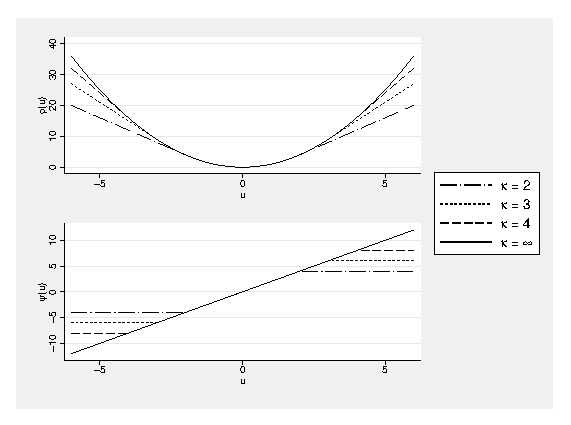
\epsfig{file=eps/4/2}
    \caption{Huber loss function $\rho_{\kappa}^{\stsc{H}}$ and score function $\psi_{\kappa}^{\stsc{H}}$}
    \label{fig:rho_psi_Huber}
\end{figure}

\begin{figure}[h!]
    \centering
    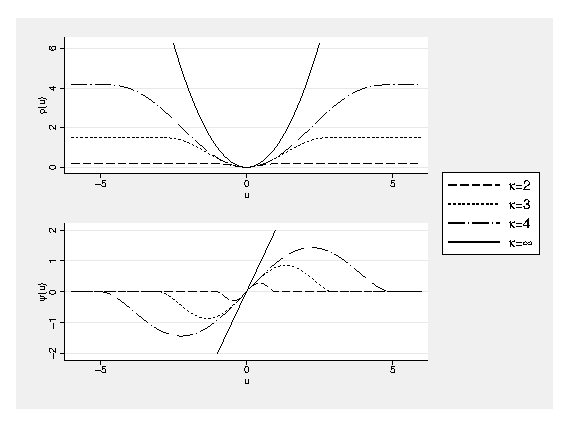
\epsfig{file=eps/4/3}
    \caption{Tukey-Biweight loss function $\rho_{\kappa}^{\stsc{B}}$ and score function $\psi_{\kappa}^{\stsc{B}}$}
    \label{fig:rho_psi_Biweight}
\end{figure}

The main advantage of monotone score functions $\psi$ is that all solutions of
(\ref{eq:M_equations}) are solutions of (\ref{eq:M_min}). In the case of
redescending score functions $\psi$, the estimating equations
(\ref{eq:M_equations}) may have multiple solutions corresponding to multiple
local minima of $\sum_{i=1}^{n}\rho(r_{i}(\boldsymbol\beta)/\sthat{\sigma})$,
and generally only one of them (the “good” solution) corresponds to the global
minimizer $\sthat{\boldsymbol\beta}_{\stsc{M};\rho}$ defined by
(\ref{eq:M_min}), which makes the computation of the \stsc{M} estimate
considerably more complex.

\begin{stremark}
Applying the \stsc{M} estimation procedure in the particular case of the
location-scale model (\ref{eq:location_scale_model}) leads to the \stsc{M}
\emph{estimators of location and scale}---we just mentioned the existence of
these estimators in the previous chapter. The interested reader will find some
results relative to these specific estimators in appendix
\ref{sec:robreg:appendix1} at the end of this chapter.
\end{stremark}

\subsection{M estimation as a generalization of maximum likelihood (ML) estimation}

The \stsc{M} estimation as defined above may be seen, as already explained, as
a generalization of the \stsc{LS} or \stsc{LAD} estimation, but also as a
generalization of the maximum-likelihood (\stsc{ML}) estimation (see, for
instance, \citealp{maronna:etal:2006}). Indeed, assuming model
(\ref{eq:location_scale_regr_model}) with fixed $\stvec{x}_{i}$ and with
$\nu_{i}$, $i = 1, \dots, n$, i.i.d.\ of density $f_{0,1}$, the likelihood of
the sample $\{y_{1}, \dots, y_{n}\}$ is given by                                \todo{Couldn't we also just use unspecified $f$ instead of $f_{0,1}$?}
\[
    \frac{1}{\sigma^{n}}\prod\limits_{i=1}^{n}
    f_{0,1}\left(\frac{y_{i}-\stvec{x}_{i}'\boldsymbol\beta}{\sigma}\right)
\]
Hence, maximum likelihood estimation of the parameters $\boldsymbol\beta$
and $\sigma$ consists in looking for
%
\begin{align}
    \left(\sthat{\boldsymbol\beta}_{\stsc{ML}}',\sthat{\sigma}_{\stsc{ML}}\right)'
    &= \arg\max_{\boldsymbol\beta,\sigma} \frac{1}{\sigma^{n}} \prod\limits_{i=1}^{n}
        f_{0,1}\left(\frac{y_{i}-\stvec{x}_{i}'\boldsymbol\beta}{\sigma}\right)
    \nonumber\\
    &= \arg\max_{\boldsymbol\beta,\sigma} \left[\sum_{i=1}^{n}
        \ln f_{0,1}\left(\frac{y_{i}-\stvec{x}_{i}'\boldsymbol\beta}{\sigma}\right) - n\ln\sigma\right]
    \nonumber\\
    & = \arg\min_{\boldsymbol\beta,\sigma} \left[\sum_{i=1}^{n}
        \rho_{\stsc{ML}}\left(\frac{r_{i}(\boldsymbol\beta)}{\sigma}\right) + n\ln\sigma\right]
    \label{eq:ML_beta_sigma_min}
\end{align}
%
where $\rho_{\stsc{ML}}(u) = -\ln f_{0,1}(u)$. If $\sigma$ is known, the
minimization problem simply becomes
%
\begin{equation}\label{eq:ML_beta_min}
    \sthat{\boldsymbol\beta}_{\stsc{ML}} 
        = \arg\min_{\boldsymbol\beta}\sum_{i=1}^{n} 
            \rho_{\stsc{ML}}\left(\frac{r_{i}(\boldsymbol\beta)}{\sigma}\right)
\end{equation}
%
and $\sthat{\boldsymbol\beta}_{\stsc{ML}}$ is solution of the estimating
equations system
\[
    \sum_{i=1}^{n} \psi_{\stsc{ML}}\left(\frac{r_{i}(\boldsymbol\beta)}{\sigma}\right) \stvec{x}_{i} = \mathbf{0}
\]
where $\psi_{\stsc{ML}}(u) = \rho_{\stsc{ML}}'(u) = - (1/f_{0,1}(u))
f_{0,1}'(u)$. If $f_{0,1}$ is the standard normal density function,
$\sthat{\boldsymbol\beta}_{\stsc{ML}}$ coincides with
$\sthat{\boldsymbol\beta}_{\stsc{LS}}$. If $f_{0,1}$ is the density function of
the Laplace distribution, that is, if $f_{0,1}(u) =
\frac{1}{\sqrt{2}}\exp(-\sqrt{2}|u|)$, $u\in\mathbb{R}$, then
$\sthat{\boldsymbol\beta}_{\stsc{ML}}$ is equal to
$\sthat{\boldsymbol\beta}_{\stsc{LAD}}$.

If $\sigma$ is not known but is estimated beforehand and fixed in
(\ref{eq:ML_beta_min}), the estimating equations system becomes
\[
    \sum_{i=1}^{n} \psi_{\stsc{ML}}\left(\frac{r_{i}(\boldsymbol\beta)}{\sthat{\sigma}}\right) \stvec{x}_{i} = \mathbf{0}
\]
Note that, if $\boldsymbol\beta$ and $\sigma$ are estimated simultaneously,
the estimating equations system related to (\ref{eq:ML_beta_sigma_min}) is
%
\begin{equation}\label{eq:ML_beta_sigma_equations}
    \begin{cases}
        \sum\limits_{i=1}^{n} \psi_{\stsc{ML}}\left(\frac{r_{i}(\boldsymbol\beta)}{\sigma}\right) \stvec{x}_{i} = \mathbf{0}\\
        \frac{1}{n} \sum\limits_{i=1}^{n} \rho_{\stsc{ML};\mathrm{scale}}\left(\frac{r_{i}(\boldsymbol\beta)}{\sigma}\right) = \delta
    \end{cases}
\end{equation}
%
where $\rho_{\stsc{ML};\mathrm{scale}}(u) = u\psi_{\stsc{ML}}(u)$ and
$\delta=1$.

\subsection{Practical implementation of M estimates}
\label{subsec:practical_implementation_Mestimate}

Let us first assume, for simplicity, that the scale parameter $\sigma$ is
known. In that case, the regression M-estimate
$\sthat{\boldsymbol\beta}_{\stsc{M};\rho}$ is solution of the estimating
equations system (\ref{eq:M_equations}) where $\sthat{\sigma}$ is replaced by
$\sigma$. Defining the weight function $w$ by
\[
    w(u) = 
    \begin{cases}
        \frac{\psi(u)}{u} & \text{if $u\neq0$}\\
        \psi'(0)          & \text{if $u=0$}
    \end{cases}
\]
the estimating system (\ref{eq:M_equations}) can be rewritten as
%
\begin{equation}\label{eq:weighted_LS_equations}
    \sum_{i=1}^{n} w_{i} r_{i}(\boldsymbol\beta) \stvec{x}_{i} = \mathbf{0}
\end{equation}
%
where $w_{i} = w(r_{i}(\boldsymbol\beta)/\sigma)$. Hence, the equations to
solve in the \stsc{M} estimation procedure appear as \emph{weighted} versions
of the normal equations (\ref{eq:LS_equations}) related to \stsc{LS}
estimation, and if the $w_{i}$'s were known, the equations
(\ref{eq:weighted_LS_equations}) could be solved by applying \stsc{LS} to
$\sqrt{w_{i}}y_{i}$ and $\sqrt{w_{i}}\stvec{x}_{i}$. But the weights $w_{i}$
are functions of $\boldsymbol\beta$ and depend upon the data, and hence are not
known. So we have to use an iterative procedure. Using an initial estimate
$\sthat{\boldsymbol\beta}_0$ for $\boldsymbol\beta$ (for instance, the
\stsc{LAD} estimate of $\boldsymbol\beta$), the weights can be computed and
serve as the start of an \emph{iteratively reweighted least squares algorithm}
(\stsc{IRWLS}). Note however that the latter is guaranteed to converge to the
global minimum of (\ref{eq:M_min}) only if the loss function $\rho$ is convex
on the whole real line $\mathbb{R}$ (which is the case for the
$\rho_{c}^{\stsc{H}}$ functions introduced by Huber).\footnote{In the case of
a convex loss function $\rho$, the convergence of the algorithm to the global
minimum of (\ref{eq:M_min}) is guaranteed whatever the starting point
$\sthat{\boldsymbol\beta}_0$.}

If $\sigma$ is not known, it can be estimated (in a robust way) beforehand
using the residuals $r_{i}(\sthat{\boldsymbol\beta}_0)$, $i = 1, \dots, n$,
and then fixed in the iterative procedure described above. It is of course
also possible to estimate simultaneously $\boldsymbol\beta$ and $\sigma$ in
this procedure, by updating $\sthat{\sigma}$ at each iteration (see
\citealp{maronna:etal:2006} for more details).

\subsubsection{Regression M estimate with preliminary scale estimation}

In practice, we may take the \stsc{LAD} estimate as initial estimate
$\sthat{\boldsymbol\beta}_0$ for $\boldsymbol\beta$ (recall that the \stsc{LAD}
estimate does not require estimating a scale). Then we may estimate $\sigma$
using normalized \stsc{MAD} of the residuals
$r_{i}(\sthat{\boldsymbol\beta}_0)$. More precisely, we may take
\[
    \sthat{\sigma} = 1.4826 \cdot 
    \med_{i}\left(\left|r_{i}(\sthat{\boldsymbol\beta}_0)\right|; r_{i}(\sthat{\boldsymbol\beta}_0) \neq 0\right)
\]
The reason for using only \emph{non null} residuals is that, since at least
$(p+1)$ residuals $r_{i}(\sthat{\boldsymbol\beta}_0) =
r_{i}(\sthat{\boldsymbol\beta}_{\stsc{LAD}})$ are equal to zero, determining
the \stsc{MAD} of the $n$ residuals could lead to underestimating $\sigma$ when
$p$ is large.

Since $\sthat{\boldsymbol\beta}_{\stsc{LAD}}$ is regression, scale and
affine equivariant, it is easy to show that
%
\begin{align*}
    \sthat{\sigma}(\stmat{X}, \stvec{y} + \stmat{X}\boldsymbol\gamma)
        &= \sthat{\sigma}(\stmat{X}, \stvec{y})
        \qquad\text{for all $\boldsymbol\gamma \in \mathbb{R}^{p+1}$}\\
    \sthat{\sigma}(\stmat{X}\stmat{A}, \stvec{y})
        &= \sthat{\sigma}(\stmat{X}, \stvec{y})
        \qquad\text{for any nonsingular $\mathbf{A} \in \mathbb{R}^{(p+1)\times(p+1)}$}
\end{align*}
%
and
\[
    \sthat{\sigma}(\stmat{X}, \lambda\stvec{y}) 
    = |\lambda| \sthat{\sigma} (\stmat{X}, \stvec{y})
    \qquad\text{for all $\lambda\in\mathbb{R}$}
\]
Hence, $\sthat{\sigma}$ is regression and affine invariant, as well as scale
equivariant, which ensures the regression, scale end affine equivariance of
the \stsc{M} estimator $\sthat{\boldsymbol\beta}_{\stsc{M};\rho}$.


\subsection{Regression quantiles as regression M estimates}

Let
\[
    \rho_{\alpha}(u)=
    \begin{cases}
        \alpha u     & \text{if $u\geq0$}\\
        -(1-\alpha)u & \text{if $u<0$}
    \end{cases}
\]
for $\alpha \in (0,1)$. \citet{Koenker:1978} defined the \emph{regression $\alpha$-quantile} 
$\sthat{\boldsymbol\beta}_{\alpha}$ as follows:
%
\begin{equation}\label{eq:quantile_regr_min}
    \sthat{\boldsymbol\beta}_{\alpha} 
    = \arg\min_{\boldsymbol\beta} \sum_{i=1}^{n} \rho_{\alpha}(y_{i}-\stvec{x}_{i}'\boldsymbol\beta)
\end{equation}

The case $\alpha=0.5$ corresponds to the \stsc{LAD} estimate. Assume the model
\[
    y_{i} = \stvec{x}_{i}' \boldsymbol\beta_{\alpha} + \epsilon_{i},
    \qquad i = 1, \dots, n
\]
where the $\stvec{x}_{i}$'s are fixed and the $\alpha$-quantile of
$\epsilon_{i}$ is zero; this is equivalent to assuming that the
$\alpha$-quantile of $y_{i}$ is, conditionally to $\stvec{x}_{i}$, equal to
$\stvec{x}_{i}'\boldsymbol\beta_{\alpha}$. Then $\widehat
{\boldsymbol\beta}_{\alpha}$ defined by (\ref{eq:quantile_regr_min}) is an
estimate of $\boldsymbol\beta_{\alpha}$. It may be seen as a generalization of
the \stsc{LAD} estimate as well as a specific case of \stsc{M} estimate.

Regression quantiles are especially useful with heteroskedastic data. There is
a very large literature on regression quantiles; see, for instance,
\citet{Koenker:2005}.

\subsection{Monotone vs. redescending M estimators}

As already mentioned, taking a loss function $\rho(u)$ in the minimization
problem (\ref{eq:M_min}) that is less rapidly increasing than the square
function provides a certain robustness of the regression \stsc{M} estimate with
respect to the vertical points. But what about the robustness of
$\sthat{\boldsymbol\beta}_{\stsc{M};\rho}$ with respect to leverage points? To
answer to this question, let us recall that
$\sthat{\boldsymbol\beta}_{\stsc{M};\rho}$ is solution of the estimating
equations system (\ref{eq:M_equations}).

It is easy to see that \emph{monotone} \stsc{M} estimates break down in
presence of a single bad leverage point. Indeed, if $\psi(u)$ is a monotone
function, an $\stvec{x}$-outlier will dominate the solution of
(\ref{eq:M_equations}) in the following sense: if for some $i$, $\stvec{x}_{i}$
is “much larger than the rest”, then in order to make the sum in the left part
of (\ref{eq:M_equations}) to zero, the residual
$r_{i}(\sthat{\boldsymbol\beta}) = y_{i} -
\stvec{x}_{i}'\sthat{\boldsymbol\beta}$ must be near zero, that is, the
regression hyperplane has to fit the point $(\stvec{x}_{i}, y_{i})$ as well as
possible, and hence $\sthat{\boldsymbol\beta}$ is essentially determined by
this leverage point $(\stvec{x}_{i}, y_{i})$.

This does not happen with the \emph{redescending} \stsc{M} estimate since the
use of a function $\psi$ that vanishes for “outlying” residuals allows to find
a solution $\widehat{\boldsymbol\beta}_{\stsc{M};\rho}$ of
(\ref{eq:M_equations}) which is not affected by the presence of a bad leverage
point $(\stvec{x}_{i}, y_{i})$ in the data set. Hence, from the robustness
point of view, the redescending regression \stsc{M} estimators are more interesting
than the monotone \stsc{M} estimators. Unfortunately, as already explained, the
practical implementation of \stsc{M} estimators is less easy for the
redescending than for the monotone ones.

\subsection{GM estimation}

Other approaches have been considered to limit the influence of leverage points
on the estimation of the regression coefficients. For instance, defining
$\underline{\stvec{x}}_{i} = (x_{i1}, \ldots, x_{ip})'$ such that
$\stvec{x}_{i} = (1,\underline{\stvec{x}}_{i}')'$, a simple way to robustify a
monotone \stsc{M} estimate is to downweight the influential
$\underline{\stvec{x}}_{i}$'s to prevent them from dominating the estimating
equations. Hence we may define an estimate as solution of
\begin{equation}\label{eq:GM_equations_1}
    \sum_{i=1}^{n} \psi\left(\frac{r_{i}(\boldsymbol\beta)}{\sthat{\sigma}}\right) 
    \widetilde{w}(d(\underline{\stvec{x}}_{i})) \stvec{x}_{i} = \mathbf{0}
\end{equation}
where $\widetilde{w}$ is a weight function and $d(\underline{\stvec{x}}_{i})$
is some measure of the “largeness” of $\underline{\stvec{x}}_{i}$. Here $\psi$
is monotone and $\sthat{\sigma}$ is simultaneously estimated by an \stsc{M}
estimating equation of the form
\[
    \frac{1}{n}\sum_{i=1}^{n} \rho_{\mathrm{scale}}\left(\frac{r_{i}(\boldsymbol\beta)}{\sigma}\right)  = \delta
\]
In order to bound the effect of influential points, $\widetilde{w}$ must be
such that $\widetilde{w}(t)t$ is bounded.

More generally, we may let the weights depend on the residuals as well as on
the predictor variables, and use a \emph{generalized} \stsc{M} estimate
(\stsc{GM} estimate) $\sthat{\boldsymbol\beta}_{\stsc{GM}}$ defined as solution
of
%
\begin{equation}\label{eq:GM_equations_2}
    \sum_{i=1}^{n}\eta\left(d(\underline{\stvec{x}}_{i}), \frac{r_{i}(\boldsymbol\beta)}{\sthat{\sigma}}\right)
    \stvec{x}_{i} = \mathbf{0}
\end{equation}
%
where for each $s$, $\eta(s,u)$ is a nondecreasing and bounded $\psi$-function
of $u$. The estimating equations system (\ref{eq:GM_equations_1}) may be seen
as a particular case of (\ref{eq:GM_equations_2}) when choosing $\eta(s,u) =
\widetilde{w}(s) \psi(u)$. This particular choice corresponds to the class of
\emph{Mallows estimates} (see \citealp{Mallows:1975}) which has been
extensively studied in the literature.

The most usual way to measure the “largeness” of $\underline{\stvec{x}}_{i}$,
$i=1, \dots, n$, is to take the \emph{leverage} of $\underline{\stvec{x}}_{i}$,
that is, to consider
%
\begin{equation}
    \label{eq:leverage}
    d(\underline{\stvec{x}}_{i}) = 
    \sqrt{\left(\underline{\stvec{x}}_{i} - \sthat{\boldsymbol\mu}_{\underline{\stvec{x}}}\right)'
    \sthat{\boldsymbol\Sigma}_{\underline{\stvec{x}}}^{-1}
    \left(\underline{\stvec{x}}_{i} - \sthat{\boldsymbol\mu}_{\underline{\stvec{x}}}\right)}
\end{equation}
%
where $\sthat{\boldsymbol\mu}_{\underline{\stvec{x}}}$ and
$\sthat{\boldsymbol\Sigma}_{\underline{\stvec{x}}}$ are a robust location
vector and robust dispersion matrix of the $\underline{\stvec{x}}_{i}$'s,
respectively (see chapter~\ref{chap:mv}). If
$\sthat{\boldsymbol\mu}_{\underline{\stvec{x}}}$ and
$\sthat{\boldsymbol\Sigma}_{\underline{\stvec{x}}}$ are the sample mean and
covariance matrix, $d(\cdot)$ is known as the Mahalanobis distance.

As stated in \citet{rousseeuw:leroy:1987}, the \stsc{GM} estimators were
constructed in the hope of bounding the influence of a single outlying
observation. Relying on this, optimal choices of $\psi$ and $\widetilde{w}$
were made (see, among others, \citealp{Ronchetti:Rousseeuw:1985} for a survey).
However, \citet{Maronna:1979} have proven that the breakdown point of all
\stsc{GM} estimators is non-zero but decreases as a function of $p$ (i.e., the
breakdown point is less or equal to $1/(p+1)$) pointing out that a
\stsc{GM} estimator is interesting to be used only when the number of
explanatory variables is very small. Furthermore, \citet{maronna:etal:2006}
show that, to obtain affine equivariance of
$\sthat{\boldsymbol\beta}_{\stsc{GM}}$, it is necessary that
$\sthat{\boldsymbol\mu}_{\underline{\stvec{x}}}$ and
$\sthat{\boldsymbol\Sigma}_{\underline{\stvec{x}}}$ used in (\ref{eq:leverage})
are affine equivariant, which presents the same computational difficulties as
for redescending \stsc{M} estimates and reduce substantially the appeal of this
estimator.

\section{Robust regression with a high breakdown point}

As explained previously, \stsc{LS} regression is now being criticized more and
more for its dramatic lack of robustness. Indeed, one single outlier can have
an arbitrarily large effect on the estimate: the breakdown point
$\varepsilon^*$ of $\sthat{\beta}_{\stsc{LS}}$ is clearly equal to zero.
Although \stsc{LAD} regression protects against outlying $y_{i}$, it cannot
cope with grossly aberrant values of $\stvec{x}_{i}$: \stsc{LAD} regression
yields the same value $\varepsilon^*=0$ as \stsc{LS}. \stsc{M} estimation
provides a certain robustness with respect to vertical points, but not with
respect to bad leverage points when the loss function $\rho$ is unbounded: the
breakdown point $\varepsilon^*$ associated with a monotone \stsc{M} estimator
is then still equal to zero.

Because of this vulnerability to bad leverage points, generalized \stsc{M}
estimators (\stsc{GM} estimators) were introduced, with the basic purpose of
bounding the influence of outlying $\stvec{x}_{i}$. It turns out, however, that
the GM-estimators now in use have a breakdown point of at most $1/(p+1)$, where
$(p+1)$ is the dimension of $\stvec{x}_{i}$. Various other estimators have been
proposed by \citet{Theil:1950}, \citet{Brown:1951}, \citet{Sen:1968},
\citet{Jaeckel:1972}, and \citet{Andrews:1974}, but none of them achieves
$\varepsilon^*=30\%$ in the case of simple regression ($p=1$).

All of this raises the question whether robust regression with a high breakdown
point is at all possible. The affirmative answer was given by
\citet{Siegel:1982}, who proposed an estimator (the \emph{repeated median})
with a 50\% breakdown point. Note that 50\% is the best that can be expected:
for larger amounts of contamination, it becomes impossible to distinguish
between the “good” and the “bad” parts of the sample. Siegel's estimator can be
calculated explicitly but is not equivariant for linear transformations of the
$\stvec{x}_{i}$ (it is not affine equivariant). This explains why we do not
study this estimator in more details and prefer to present other estimators
introduced by Rousseeuw and Yohai, and all based on a robust scale measure.

\subsection{LTS and LMS estimation}

Robustness can be achieved by tackling the estimation of the regression
parameters vector $\boldsymbol\beta$ from a different perspective. We know that
\stsc{LS} estimation is based on the minimization of the variance of the
residuals. However, since the variance is highly sensitive to outliers,
LS-estimate will be sensitive to them as well. An interesting idea would then
consist in minimizing a measure of the residual dispersion
$s(r_{1}(\boldsymbol\beta), \dots, r_{n}(\boldsymbol\beta))$ that is less
sensitive to extreme residuals.

Relying on this idea, \citet{Rousseeuw:1983} introduced the \emph{Least Trimmed
Sum of Squares} (\stsc{LTS}) estimator which is based on the minimization of a
trimmed variance of the residuals:
\[
    \sthat{\boldsymbol\beta}_{\stsc{LTS}}
     = \arg\min_{\boldsymbol\beta}s_{\stsc{LTS}}(r_{1}(\boldsymbol\beta), \dots, r_{n}(\boldsymbol\beta))
\]
with
\[
    s_{\stsc{LTS}}(r_{1}(\boldsymbol\beta), \dots, r_{n}(\boldsymbol\beta))
    = \sqrt{\frac{1}{\lceil\alpha n\rceil} 
      \sum_{i=1}^{\lceil\alpha n\rceil}r_{(i)}^{2}(\boldsymbol\beta)}
\]
where $1/2 \leq \alpha \leq 1$ and $r_{(1)}^{2}(\boldsymbol\beta) \leq \dots
\leq r_{(n)}^{2}(\boldsymbol\beta)$ are the ordered squared residuals. The
constant $\alpha$ determines the trade-off between the robustness and the
efficiency of the estimator. Indeed, if $\alpha$ tends to one, the \stsc{LTS}
estimator tends to the \stsc{LS} estimator. In contrast, if $\alpha = 1/2$, the
\stsc{LTS} estimator will resist up to 50\% of outlying data and, consequently,
will have a breakdown point equal to 50\%. Unfortunately, even if
$\sthat{\boldsymbol\beta}_{\stsc{LTS}}$ converges to $\boldsymbol\beta$ at a
rate of $1/\sqrt{n}$, its efficiency is low (under Gaussian conditions, the
asymptotic relative efficiency of $\sthat{\boldsymbol\beta}_{\stsc{LTS}}$ with
respect to $\sthat{\boldsymbol\beta}_{\stsc{LS}}$ reaches only 7\% when 50\% of
the data are trimmed).

Despite its relatively low efficiency, the \stsc{LTS} estimator is quite popular
because it can be quickly computed using the \emph{Fast-lts algorithm}
developed by \citet{rousseeuw&vdriessen99}; this estimator is available in
Stata through the command \stcmd{robreg lts}.

Following the same idea, \citet{rousseeuw:1984} introduced the \emph{Least Median
Squares} (\stsc{LMS}) estimator based on the minimization of the median of
the squared residuals:\footnote{The variance of the residuals corresponds to
the arithmetic mean of the squared residuals; why not replace the mean by the
more robust median?}
\[
    \sthat{\boldsymbol\beta}_{\stsc{LMS}} 
    = \arg\min_{\boldsymbol\beta} s_{\stsc{LMS}}(r_{1}(\boldsymbol\beta), \dots, r_{n}(\boldsymbol\beta))
\]
with
\[
    s_{\stsc{LMS}}(r_{1}(\boldsymbol\beta), \dots, r_{n}(\boldsymbol\beta)) 
    = \sqrt{\mathrm{med}_{i}\;r_{i}^{2}(\boldsymbol\beta)}
\]
\stsc{LMS} satisfies $\varepsilon^* = 50\%$ but has unfortunately a very low
efficiency because of its $1/\sqrt[3]{n}$ convergence rate. The \stsc{LMS}
estimator is available in Stata through the command \stcmd{robreg lms}.

\alert{[Add paragraph on LQS, as this is also supported by robreg.]}

\subsection{S estimation}

Following always the same principle, \citet{rousseeuw:yohai:1984} have
introduced a more general class of estimators: the regression
\stsc{S} estimators.

In order to well understand the basic intuition behind the \stsc{S} estimation,
let us consider once again the \stsc{LS} estimation. For \stsc{LS} estimation,
we actually are looking for the value of the regression coefficients vector
$\boldsymbol{\beta}$ that minimizes the variance (or standard deviation) of the
residuals $r_{i}(\boldsymbol\beta)$, $i = 1, \dots, n$. More formally, we have
\[
    \sthat{\boldsymbol\beta}_{\stsc{LS}} 
    = \arg\min_{\boldsymbol\beta} s_{\stsc{LS}}(r_{1}(\boldsymbol\beta), \dots, r_{n}(\boldsymbol\beta))
\]
with
\[
    s_{\stsc{LS}}(r_{1}(\boldsymbol\beta), \dots, r_{n}(\boldsymbol\beta)) 
    = \sqrt{\frac{1}{n}\sum_{i=1}^{n} r_{i}^{2}(\boldsymbol\beta)}
\]
The dispersion measure $s_{\stsc{LS}}$ may be characterized as follows: given
the realizations $e_{1}, \dots, e_{n}$ of $n$ i.i.d.\ random variables whose
distribution is characterized by a mean equal to zero and a scale parameter
$\sigma$, the dispersion measure $s_{\stsc{LS}}(e_{1}, \dots, e_{n})$ of the
sample is an estimate of $\sigma$ satisfying the equality
\[
    \frac{1}{n}\sum_{i=1}^{n} \left(\frac{e_{i}}{s_{\stsc{LS}}(e_{1}, \dots, e_{n})}\right)^{2} = 1
\]
or, taking $\rho(u) = u^{2}$,
\[
    \frac{1}{n}\sum_{i=1}^{n} \rho\left(\frac{e_{i}}{s_{\stsc{LS}}(e_{1}, \dots, e_{n})}\right) = 1
\]
Moreover, if $u \sim \mathcal{N}(0,1)$, then $E(\rho(u)) = E(u^{2}) = 1$.

The \stsc{S} estimation procedure proposed by \citet{rousseeuw:yohai:1984}
relies on the same philosophy as the one underlying the \stsc{LS} estimation,
but introduces robustness by using specific robust residual dispersion measures
which correspond to \stsc{M} estimators of the scale parameter $\sigma$. More
formally, given the realizations $e_{1}, \dots, e_{n}$ of $n$ i.i.d.\ random
variables with scale parameter $\sigma$ (and a location parameter equal to
zero), the \stsc{M} estimate $\sthat{\sigma}_{\rho}$ of $\sigma$ is the
measure of dispersion $s_{\rho}(e_{1}, \dots, e_{n})$ defined as the solution
of the equation
%
\begin{equation}\label{eq:M_scale_equation}
    \frac{1}{n}\sum_{i=1}^{n} \rho\left(\frac{e_{i}}{s_{\rho}(e_{1}, \dots, e_{n})}\right) = \delta
\end{equation}
%
where
\begin{itemize}
    \item the function $\rho(\cdot)$ is positive, even (such that
    $\rho(0) = 0$), non decreasing for positive values and bounded;

    \item the constant $\delta$ is defined such that $\sthat{\sigma}_{\rho} =
    s_{\rho}(e_{1}, \dots, e_{n})$ is a consistent estimate of $\sigma$ for the
    Gaussian regression model (generally $\delta$ is defined by $\delta =
    E(\rho(u))$ for $u \sim \mathcal{N}(0,1)$; the consistency parameter
    $\delta$ would therefore be nothing else than the population counterpart of
    the lefthand side of equation (\ref{eq:M_scale_equation})).
\end{itemize}

Then \citet{rousseeuw:yohai:1984} defined an \stsc{S} estimate of
$\boldsymbol\beta$ by
\[
    \sthat{\boldsymbol\beta}_{\mathrm{S};\rho} 
    = \arg\min_{\boldsymbol\beta}s_{\rho} (r_{1}(\boldsymbol\beta), \dots, r_{n}(\boldsymbol{\beta}))
\]
where $s_{\rho}$ is a measure of dispersion defining a scale \stsc{M} estimator, that is,
satisfying
%
\begin{equation}\label{eq:M_scale_equation_res}
    \frac{1}{n}\sum_{i=1}^{n} \rho\left(\frac{r_{i}(\boldsymbol{\beta})}%
        {s_{\rho}(r_{1}(\boldsymbol\beta), \dots, r_{n}(\boldsymbol\beta))}\right) = \delta
    \qquad\text{for all $\boldsymbol\beta \in \mathbb{R}^{p+1}$}
\end{equation}


One important fact is that an S-estimate of $\boldsymbol\beta$ is also an
M-estimate. More precisely, $\sthat{\boldsymbol\beta}_{\mathrm{S};\rho}$
is an M-estimate (in the sense of (\ref{eq:M_min})) in that
\begin{equation}
\sum_{i=1}^{n}\rho\left(  \frac{r_{i}\left(  \sthat{\boldsymbol\beta%
}_{\mathrm{S};\rho}\right)  }{\sthat{\sigma}_{\rho}}\right)  \leq\sum
_{i=1}^{n}\rho\left(  \frac{r_{i}\left(  \widetilde{\boldsymbol\beta%
}\right)  }{\sthat{\sigma}_{\rho}}\right)  \hspace{2cm}\text{for all
}\widetilde{\boldsymbol\beta}\in\mathbb{R}^{p+1}, \label{eq:S_Minequality_1}%
\end{equation}
where the residuals are standardized by the same scale M-estimate
$\sthat{\sigma}_{\rho}=s_{\rho}\left(  r_{1}\left(  \widehat
{\boldsymbol\beta}_{\mathrm{S};\rho}\right)  ,\ldots,r_{n}\left(
\sthat{\boldsymbol\beta}_{\mathrm{S};\rho}\right)  \right)  $ of $\sigma$
on both sides of the inequation (\ref{eq:S_Minequality_1}). Indeed,
$\sthat{\boldsymbol\beta}_{\mathrm{S};\rho}$ minimizes the residual
dispersion measure $s_{\rho}\left(  r_{1}(\boldsymbol\beta),\ldots
,r_{n}(\boldsymbol\beta)\right)  $ which satisfies
(\ref{eq:M_scale_equation_res}). This means that, if we denote $\widehat
{\sigma}_{\rho}=s_{\rho}\left(  r_{1}\left(  \sthat{\boldsymbol\beta%
}_{\mathrm{S};\rho}\right)  ,\ldots,r_{n}\left(  \sthat{\boldsymbol\beta%
}_{\mathrm{S};\rho}\right)  \right)  $ and $\widetilde{\sigma}_{\rho}=s_{\rho
}\left(  r_{1}\left(  \widetilde{\boldsymbol\beta}\right)  ,\ldots
,r_{n}\left(  \widetilde{\boldsymbol\beta}\right)  \right)  $ for
$\widetilde{\boldsymbol\beta}\in\mathbb{R}^{p+1}$, we have $\sthat{\sigma
}_{\rho}\leq\widetilde{\sigma}_{\rho}$ and
\[
\sum_{i=1}^{n}\rho\left(  \frac{r_{i}\left(  \sthat{\boldsymbol\beta%
}_{\mathrm{S};\rho}\right)  }{\sthat{\sigma}_{\rho}}\right)  =n\delta
=\sum_{i=1}^{n}\rho\left(  \frac{r_{i}\left(  \widetilde{\boldsymbol\beta%
}\right)  }{\widetilde{\sigma}_{\rho}}\right)  .
\]
Then, since $\rho$ is monotone and $\sthat{\sigma}_{\rho}\leq\widetilde
{\sigma}_{\rho}$, we necessarily have
\[
\sum_{i=1}^{n}\rho\left(  \frac{r_{i}\left(  \sthat{\boldsymbol\beta%
}_{\mathrm{S};\rho}\right)  }{\sthat{\sigma}_{\rho}}\right)  =\sum_{i=1}%
^{n}\rho\left(  \frac{r_{i}\left(  \widetilde{\boldsymbol\beta}\right)
}{\widetilde{\sigma}_{\rho}}\right)  \leq\sum_{i=1}^{n}\rho\left(  \frac
{r_{i}\left(  \widetilde{\boldsymbol\beta}\right)  }{\sthat{\sigma}_{\rho
}}\right)  ,
\]
which proves (\ref{eq:S_Minequality_1}).

If $\rho$ has a derivative $\psi$, it follows that $\sthat{\boldsymbol{\beta
}}_{\mathrm{S};\rho}$ is also an M-estimate in the sense of
(\ref{eq:M_equations}), but with the condition that the scale parameter
$\sigma$ is estimated simultaneously with $\boldsymbol\beta$. More formally,
$\boldsymbol\beta$ is estimated by $\sthat{\boldsymbol\beta}%
_{\mathrm{S};\rho}$ and $\sigma$ by $\sthat{\sigma}_{\rho}=s_{\rho}\left(
r_{1}\left(  \sthat{\boldsymbol\beta}_{\mathrm{S};\rho}\right)
,\ldots,r_{n}\left(  \sthat{\boldsymbol\beta}_{\mathrm{S};\rho}\right)
\right)  $, with $\sthat{\boldsymbol\beta}_{\mathrm{S};\rho}$ and
$\sthat{\sigma}_{\rho}$ such that
\[
\left\{
\begin{array}
[c]{l}%
\sum\limits_{i=1}^{n}\psi\left(  \dfrac{r_{i}\left(  \widehat
{\boldsymbol\beta}_{\mathrm{S};\rho}\right)  }{\sthat{\sigma}_{\rho}%
}\right)  \stvec{x}_{i}=\mathbf{0}\\
\dfrac{1}{n}\sum\limits_{i=1}^{n}\rho\left(  \dfrac{r_{i}\left(
\sthat{\boldsymbol\beta}_{\mathrm{S};\rho}\right)  }{\sthat{\sigma
}_{\rho}}\right)  =\delta.
\end{array}
\right.
\]
Note that, taking $\rho\left(  u\right)  =u^{2}$ and $\delta=1$, we retrieve
the standard LS minimization problem.

The choice of $\rho\left(  \cdot\right)  $ is crucial to have good robustness
properties\footnote{Note that the function $\rho$ defining the S-estimator
needs to be \emph{bounded} to get a positive breakdown point for the
regression estimator $\sthat{\boldsymbol\beta}_{\mathrm{S};\rho}$.} and a
high Gaussian efficiency. The Tukey-Biweight function defined in
(\ref{eq:Tukey_Biweight_function}), with $\kappa=1.547$, is a common choice.
This S-estimator resists to a contamination of up-to 50\% of outliers and,
hence, have a breakdown point of 50\%. Unfortunately, this S-estimator has a
Gaussian efficiency of only 28.7\%. If $\kappa=5.182$, the Gaussian efficiency
raises to 96.6\% but the breakdown point drops to 10\%. Actually an
S-estimator cannot simultaneously have a high breakdown point and a high
efficiency. In particular, H\"{o}ssjer (1992) has shown that the maximum
Gaussian asymptotic efficiency of an S-estimator with a breakdown point of
50\% is 33\%.

\subsection{MM-estimation}
\label{subsec:MM_estimation}

We have just seen that S-estimation does not allow to reach jointly a high
breakdown point and a high Gaussian efficiency. How should we then estimate
the parameters of the regression model if we aim to combine high efficiency
under normal errors with a high breakdown point? Several proposals have been
made: the \emph{MM-estimators} of Yohai (1987), the $\tau$%
\emph{-estimators} of Yohai and Zamar (1988), the \emph{constrained M (CM)
estimators} of Mendes and Tyler (1996). All these estimators can have a
Gaussian asymptotic efficiency as close to 1 as desired, and simultaneously a
breakdown point of 50\%. Gervini and Yohai (2002) proposed one estimator that
has a breakdown point of 50\% and an efficiency equal to 1.

Let us here focus our attention on the regression MM-estimators since there
are based on the M- and S-estimation procedures studied in the previous
sections. An MM-estimator is defined in two successive steps:

\begin{enumerate}
\item Take an S-estimate $\sthat{\boldsymbol\beta}_{\mathrm{S};\rho_{0}}$
with high breakdown point (but possibly low normal efficiency) where the scale
measure $s_{\rho_{0}}$ is defined by
\[
\frac{1}{n}\sum_{i=1}^{n}\rho_{0}\left(  \frac{r_{i}\left(  \boldsymbol{\beta
}\right)  }{s_{\rho_{0}}\left(  r_{1}(\boldsymbol\beta),\ldots
,r_{n}(\boldsymbol\beta)\right)  }\right)  =\delta\hspace{2cm}\text{for all
}\boldsymbol\beta\in\mathbb{R}^{p+1}%
\]
($s_{\rho_{0}}$ is associated with the function $\rho_{0}\left(  \cdot\right)
$ and the constant $\delta$). Let $\sthat{\sigma}_{\rho_{0}}=s_{\rho_{0}%
}\left(  r_{1}\left(  \sthat{\boldsymbol\beta}_{\mathrm{S};\rho_{0}%
}\right)  ,\ldots,r_{n}\left(  \sthat{\boldsymbol\beta}_{\mathrm{S}%
;\rho_{0}}\right)  \right)  $.

\item Take any other function $\rho\left(  \cdot\right)  \leq\rho_{0}\left(
\cdot\right)  $ and find the MM-estimate $\sthat{\boldsymbol\beta%
}_{\mathrm{MM};\rho_{0},\rho}$ as a local minimum of
\begin{equation}
\sum_{i=1}^{n}\rho\left(  \frac{r_{i}\left(  \boldsymbol\beta\right)
}{\sthat{\sigma}_{\rho_{0}}}\right)  \label{eq:MM_min}%
\end{equation}
such that
\begin{equation}
\sum_{i=1}^{n}\rho\left(  \frac{r_{i}\left(  \sthat{\boldsymbol\beta%
}_{\mathrm{MM};\rho_{0},\rho}\right)  }{\sthat{\sigma}_{\rho_{0}}}\right)
\leq\sum_{i=1}^{n}\rho\left(  \frac{r_{i}\left(  \sthat{\boldsymbol\beta%
}_{\mathrm{S};\rho_{0}}\right)  }{\sthat{\sigma}_{\rho_{0}}}\right)  .
\label{eq:MM_inequality}%
\end{equation}

\end{enumerate}

\begin{stremark}
The key result is given in \citet{yohai:1987}. Recall that all local minima
of (\ref{eq:MM_min}) is solution of the estimating equations
(\ref{eq:M_equations}) with $\psi\left(  u\right)  =\rho^{\prime}\left(
u\right)  $ and $\sthat{\sigma}=\sthat{\sigma}_{\rho_{0}}$:
\begin{equation}
\sum_{i=1}^{n}\psi\left(  \frac{r_{i}\left(  \boldsymbol\beta\right)
}{\sthat{\sigma}_{\rho_{0}}}\right)  \stvec{x}_{i}=\mathbf{0}.
\label{eq:MM_equations}%
\end{equation}
Yohai shows that if $\rho\left(  u\right)  \leq\rho_{0}\left(  u\right)  $ for
all $u\in%
%TCIMACRO{\U{211d} }%
%BeginExpansion
\mathbb{R}
%EndExpansion
$ and if (\ref{eq:MM_inequality}) is satisfied, then $\widehat
{\boldsymbol\beta}_{\mathrm{MM};\rho_{0},\rho}$ is consistent. Moreover, it
can be shown that the MM-estimator $\sthat{\boldsymbol\beta}%
_{\mathrm{MM};\rho_{0},\rho}$ has the same breakdown point than the
S-estimator $\sthat{\boldsymbol\beta}_{\mathrm{S};\rho_{0}}$ of the first
step, determined by the function $\rho_{0}\left(  \cdot\right)  $. If
furthermore $\sthat{\boldsymbol\beta}_{\mathrm{MM};\rho_{0},\rho}$ is any
solution of (\ref{eq:MM_equations}), then it has the same efficiency --- this
efficiency is determined by the choice of the function $\rho\left(
\cdot\right)  $ --- as the global minimum of (\ref{eq:MM_min}). In conclusion,
it is not necessary to find the absolute minimum of (\ref{eq:MM_min}) to
ensure consistency, a high breakdown point and a high efficiency.
\end{stremark}

It is common to use a Tukey-Biweight $\rho_{\kappa}^{B}\left(  \cdot\right)  $
function for both the preliminary S-estimator and the final MM-estimator. The
tuning constant $\kappa$ can be set to 1.547 for the preliminary S-estimator
to guarantee a 50\% breakdown point, and it can be set to 4.685 for the second
step MM-estimator to guarantee a 95\% asymptotic Gaussian efficiency of this
final estimator. Note however that though not breaking-down, an MM-estimator
with a very high efficiency may have a high bias \emph{under moderate
contamination}: the larger the efficiency, the larger the bias. It is
therefore important to choose the efficiency so as to maintain reasonable bias
control. Results in Section 5.9 of \citet{maronna:etal:2006} show
that an efficiency of 0.95 yields too high a bias, and hence it is safer to
choose an efficiency of 0.85 which gives a smaller bias while retaining a
sufficiently high efficiency. We will raise once again this problem of bias in
Subsection \ref{subsec:Hausman}.

\subsubsection{Numerical computation of the S- and MM-estimate}

The numerical computation of the estimate $\sthat{\boldsymbol\beta%
}_{\mathrm{MM};\rho_{0},\rho}$ at the second step of the procedure follows the
approach described in Section \ref{subsec:practical_implementation_Mestimate}:
starting with $\sthat{\boldsymbol\beta}_{\mathrm{S};\rho_{0}}$, we use the
iteratively reweighted least squares algorithm to attain a solution of the
equation (\ref{eq:MM_equations}). It may be shown (see
\citet{maronna:etal:2006} that (\ref{eq:MM_min}) decreases at each
iteration, which insures (\ref{eq:MM_inequality}). Hence, once the initial
S-estimate is computed, $\sthat{\boldsymbol\beta}_{\mathrm{MM};\rho
_{0},\rho}$ comes at almost no additional computational cost.

We programmed an S- and an MM-estimator in Stata (with Tukey-Biweight loss
function) using the fast algorithm of Salibian-Barrera and Yohai (2006) for
computing the S-estimator. Explicit formulas for the estimators are not
available and it is necessary to call on numerical optimization to compute
them. We present just below a sketch of the fast algorithm for regression
S-estimates we implemented in Stata.

Consider an estimate $\sthat{\boldsymbol\beta}_{\mathrm{S};\rho}$ defined
as
\begin{equation}
\arg\min_{\boldsymbol\beta\in%
%TCIMACRO{\U{211d} }%
%BeginExpansion
\mathbb{R}
%EndExpansion
^{p+1}}s_{\rho}\left(  r_{1}\left(  \boldsymbol\beta\right)  ,\ldots
,r_{n}\left(  \boldsymbol\beta\right)  \right)  . \label{eq:S_min}%
\end{equation}
An approximate solution of (\ref{eq:S_min}) can be obtained by finding
$\sthat{\boldsymbol\beta}$ equal to
\[
\arg\min_{\boldsymbol\beta\in\mathcal{D}_{N}}s_{\rho}\left(  r_{1}\left(
\boldsymbol\beta\right)  ,\ldots,r_{n}\left(  \boldsymbol\beta\right)
\right)
\]
where
\[
\mathcal{D}_{N}=\left\{  \sthat{\boldsymbol\beta}_{1},\ldots
,\sthat{\boldsymbol\beta}_{N}\right\}
\]
is a finite set of well selected candidates for $\sthat{\boldsymbol\beta%
}_{\mathrm{S};\rho}$. One way to select these candidates is by subsampling
elementary sets among the sample $\left(  \stvec{x}_{1},y_{1}\right)
,\ldots,\left(  \stvec{x}_{n},y_{n}\right)  $ (see \citealp{rousseeuw:1984}).
More formally, take a first random subsample of $(p+1)$
observations\footnote{Recall that $(p+1)$ is the number of regression
parameters to estimate, that is the dimension of the regression coefficients
vector $\boldsymbol\beta$ to estimate.}
\[
\left(  \stvec{x}_{i_{1}},y_{i_{1}}\right)  ,\ldots,\left(  \stvec{x}%
_{i_{(p+1)}},y_{i_{(p+1)}}\right)  ;
\]
then the candidate $\sthat{\boldsymbol\beta}_{1}$ is obtained by fitting a
hyperplane containing these $(p+1)$ points:
\[
\stvec{x}_{i_{j}}^{t}\sthat{\boldsymbol\beta}_{1}=y_{i_{j}},\hspace
{1cm}j=1,\ldots,p+1.
\]
Taking $N$ subsamples we obtain the $N$ candidates. Note that if a subsample
is collinear, it is replaced by another.

How large should $N$ be? We have to guarantee that $\mathcal{D}_{N}$ includes
at least one \textquotedblleft good\textquotedblright\ candidate with high
probability, say $\left(  1-\alpha\right)  $ (with, for example, $\alpha
=0.01$). A necessary condition to have a \textquotedblleft
good\textquotedblright\ candidate is that it comes from a clean subsample,
i.e., a subsample without outliers.

The probability of getting a clean subsample depends on the fraction of
outliers in the sample and on $p$. When the fraction of outliers in the sample
increases, the probability of getting a clean subsample decreases. Suppose the
sample contains a proportion $\xi$ of outliers. Then the probability of an
outlier-free subsample is $\gamma=(1-\xi)^{p+1}$, and the probability of at
least one clean subsample among the $N$ selected subsamples is equal to
$1-(1-\gamma)^{N}$. If we want this probability to be larger than $\left(
1-\alpha\right)  $, we must have
\[
\log\alpha\geq N\log(1-\gamma)\approx-N\gamma
\]
and hence
\begin{equation}
N\geq\frac{\left\vert \log\alpha\right\vert }{\left\vert \log\left(  1-\left(
1-\xi\right)  ^{p+1}\right)  \right\vert }\approx\frac{\left\vert \log
\alpha\right\vert }{\left(  1-\xi\right)  ^{p+1}} \label{eq:N}%
\end{equation}
for $p$ not too small (see \citealp{Salibian-Barrera:2004}). Therefore $N$
must grow exponentially with $p$.

The following observation allows to save much computing time. Suppose we have
examined $(M-1)$ subsamples and
\[
\sthat{\sigma}_{\rho;M-1}=s_{\rho}\left(  r_{1}\left(  \widehat
{\boldsymbol\beta}_{M-1}\right)  ,\ldots,r_{n}\left(  \widehat
{\boldsymbol\beta}_{M-1}\right)  \right)
\]
is the current minimum of the residual dispersion measure $s_{\rho}$. Now we
draw the $M$-th subsample which yields the candidate $\widehat
{\boldsymbol\beta}_{M}$. Let us consider $\sthat{\sigma}_{\rho;M}=s_{\rho
}\left(  r_{1}\left(  \sthat{\boldsymbol\beta}_{M}\right)  ,\ldots
,r_{n}\left(  \sthat{\boldsymbol\beta}_{M}\right)  \right)  $. Since
$\rho$ is a monotone function, the inequality $\sthat{\sigma}_{\rho
;M}<\sthat{\sigma}_{\rho;M-1}$ implies that
\begin{equation}
n\delta=\sum_{i=1}^{n}\rho\left(  \frac{r_{i}\left(  \widehat
{\boldsymbol\beta}_{M}\right)  }{\sthat{\sigma}_{\rho;M}}\right)  \geq
\sum_{i=1}^{n}\rho\left(  \frac{r_{i}\left(  \sthat{\boldsymbol\beta}%
_{M}\right)  }{\sthat{\sigma}_{\rho;M-1}}\right)  . \label{eq:S_algorithm}%
\end{equation}
Consequently, if we observe that $\sum_{i=1}^{n}\rho\left(  \frac{r_{i}\left(
\sthat{\boldsymbol\beta}_{M}\right)  }{\sthat{\sigma}_{\rho;M-1}%
}\right)  >n\delta$, this necessarily means that $\sthat{\sigma}_{\rho
;M}\geq\sthat{\sigma}_{\rho;M-1}$ and we may spare the effort of computing
the scale estimate $\sthat{\sigma}_{\rho;M}$ and discard $\widehat
{\boldsymbol\beta}_{M}$. Therefore $\sthat{\sigma}_{\rho}$ has to be
computed only for those subsamples that verify the inequality
(\ref{eq:S_algorithm}).

Although the $N$ given by (\ref{eq:N}) ensures that the approximation
$\sthat{\boldsymbol\beta}$ of $\sthat{\boldsymbol\beta}_{\mathrm{S}%
;\rho}$ has the desired breakdown point, it does not imply that it is a good
approximation to the exact S-estimate. To solve this problem, Salibian-Barrera
and Yohai (2006) have proposed a procedure based on a \textquotedblleft local
improvement\textquotedblright\ step of the resampling initial candidates. This
allows for a substantial reduction of the number of candidates required to
obtain a good approximation to the optimal solution.

This algorithm can be called in Stata either directly using the \texttt{robreg
s} function\footnote{The default values that are used in Stata for the
implementation of the fast-S algorithm are $\xi=0.2$ and $\alpha=0.01$.} or
indirectly ussing the \texttt{robreg mm} function developed to compute
MM-estimate, and invoking the \texttt{initial} option. Once the S-estimate is
obtained, the MM-estimate directly follows by applying the iteratively
reweighted least squares algorithm up to convergence. As far as inference is
concerned, standard errors robust to heteroskedasticity (and asymmetric
errors) are computed according to the formulas available in the literature
(see Section \ref{sec:inference}).

\subsection{MS-estimation}

Explicit formulas for $\sthat{\boldsymbol\beta}_{\mathrm{S};\rho}$ are
generally not available and, as explained in the previous section, empirical
implementation of S-estimation requires numerical optimization based on a
subsampling algorithm. But this method presents an Achille's heel: it becomes
inapplicable in practice when several \emph{dummy} explanatory variables are
involved in the regression model (\ref{eq:linear_regr_model}). Indeed, when
several of the explanatory variables are binary, there is a high probability
that random selection of subsamples yields collinear subsamples.

To cope with this, Maronna and Yohai (2000) have introduced the MS-estimator.
The intuition behind this estimator is simple. For the sake of clarity, let us
separate continuous and dichotomous variables in (\ref{eq:linear_regr_model})
and rewrite the regression model equation as follows:
\begin{equation}
y=\left(  \beta_{0}+\beta_{1}x_{1}+\ldots+\beta_{p_{1}}x_{p_{1}}\right)
+\left(  \beta_{1}^{\ast}x_{1}^{\ast}+\ldots+\beta_{p_{2}}^{\ast}x_{p_{2}%
}^{\ast}\right)  +\varepsilon\label{eq:linear_regr_model_MS}%
\end{equation}
where $x_{1},\ldots,x_{p_{1}}$ are $p_{1}$ continuous explanatory variables
and $x_{1}^{\ast},\ldots,x_{p_{2}}^{\ast}$ are $p_{2}$ dichotomous explanatory
variables ($p=p_{1}+p_{2}$). If $\boldsymbol{\beta=}\left(  \beta_{0}%
,\beta_{1},\ldots,\beta_{p_{1}}\right)  ^{t}$ was known in equation
(\ref{eq:linear_regr_model_MS}), then $\boldsymbol\beta^{\ast}%
\boldsymbol{=}\left(  \beta_{1}^{\ast},\ldots,\beta_{p_{2}}^{\ast}\right)
^{t}$ would be robustly estimated using a monotone M-estimator (since
$x_{1}^{\ast},\ldots,x_{p_{2}}^{\ast}$ are all dummy variables, the data set
can only contain, at worst, vertical outliers). On the other hand, if
$\boldsymbol\beta^{\ast}$ was known, then $\boldsymbol\beta$ should be
estimated using an S-estimator\footnote{Since $x_{1},\ldots,x_{p_{1}}$ are
continuous explanatory variables, we cannot assume that there are no leverage
points.} and the subsampling algorithm should not generate collinear
subsamples since all explanatory variables are continuous. The idea is then to
alternate these two estimators till convergence.

Technically speaking, an MS-regression estimate is obtained iteratively; at
the $k$-th step, we define $\sthat{\boldsymbol\beta}_{\mathrm{MS}}^{(k)}$
and $\sthat{\boldsymbol\beta}_{\mathrm{MS}}^{\ast(k)}$ as follows. Let
$s_{\rho}$ be a measure of dispersion satisfying
(\ref{eq:M_scale_equation_res}), $\stvec{x}_{i}=\left(  1,x_{i1}%
,\ldots,x_{ip_{1}}\right)  ^{t}$ and $\stvec{x}_{i}^{\ast}=\left(
x_{i1}^{\ast},\ldots,x_{ip_{2}}^{\ast}\right)  ^{t}$:
\[
\left\{
\begin{array}
[c]{l}%
\sthat{\boldsymbol\beta}_{\mathrm{MS}}^{(k)}=\arg\min_{\boldsymbol{\beta
}\in%
%TCIMACRO{\U{211d} }%
%BeginExpansion
\mathbb{R}
%EndExpansion
^{p_{1}+1}}s_{\rho}\left(  \left[  y_{i}-(\stvec{x}_{i}^{\ast})^{t}%
\sthat{\boldsymbol\beta}_{\mathrm{MS}}^{\ast(k-1)}\right]  -\stvec{x}%
_{i}^{t}\boldsymbol{\beta\ };i = 1, \dots, n\right) \\
\sthat{\boldsymbol\beta}_{\mathrm{MS}}^{\ast(k)}=\arg\min
_{\boldsymbol\beta^{\ast}\in%
%TCIMACRO{\U{211d} }%
%BeginExpansion
\mathbb{R}
%EndExpansion
^{p_{2}}}\sum_{i=1}^{n}\rho\left(  \dfrac{\left[  y_{i}-(\stvec{x}_{i}%
)^{t}\sthat{\boldsymbol\beta}_{\mathrm{MS}}^{(k-1)}\right]  -\left(
\stvec{x}_{i}^{\ast}\right)  ^{t}\boldsymbol\beta^{\ast}}{\sthat{\sigma
}^{(k-1)}}\right)  ,
\end{array}
\right.
\]
where $\sthat{\sigma}^{(k-1)}=s_{\rho}\left(  y_{i}-(\stvec{x}_{i}%
)^{t}\sthat{\boldsymbol\beta}_{\mathrm{MS}}^{(k-1)}-(\stvec{x}_{i}^{\ast
})^{t}\sthat{\boldsymbol\beta}_{\mathrm{MS}}^{\ast(k-1)}\boldsymbol{\ }%
;i = 1, \dots, n\right)  $. Note that \texttt{robreg s} and \texttt{robreg mm}
automatically recognize the presence of dummy variables among the explanatory
variables and, if appropriate, automatically apply the MS-procedure.

Unfortunately, as stated above, the price to pay for robustness is efficiency.
However this MS-estimator can be particularly helpful in the fixed effects
panel data models, as suggested by Bramati and Croux (2007).

\section{Robust inference for M-, S- and MM-estimators}
\label{sec:inference}

Consistency and asymptotic normality of M-estimators under the assumption of
i.i.d. error terms have been studied by Yohai and Maronna (1979) and for
MM-estimators by Yohai (1987). Under fairly general conditions, allowing also
for heteroskedasticity, asymptotic normality for S- and MM-estimators has been
shown by Salibian-Barrera and Zamar (2004) in the location case. Some of these
results are summarized in \citet{maronna:etal:2006} with a
distinction made between the case of \emph{fixed} predictors and the case of
\emph{random} predictors.

\citet{Croux:2003} have established the asymptotic normality of M-,
S- and MM-estimators in the regression case under quite general conditions:
they only assume that the observations $\left(  \stvec{x}_{1},y_{1}\right)
,\ldots,\left(  \stvec{x}_{n},y_{n}\right)  $ are generated by a
\emph{stationary}\footnote{A \emph{stationary} process is a stochastic
process whose joint probability distribution does not change when shifted in
time or space. Consequently, parameters such as the mean and the variance, if
they exist, also do not change over time or position . Hence, the mean and the
variance of the process do not follow trends.} and \emph{ergodic}\footnote{A
stochastic process is said to be \emph{ergodic} if its statistical
properties (such as its mean and variance) can be estimated consistently from
a single, sufficiently long sample (realization) of the process.} process $H$.
Under this assumption, the observations do not need to be independent, we may
have heteroskedasticity (the processes $\stvec{x}_{i}$ and $\varepsilon_{i}$
are not necessarily independent) and the distribution of the error terms is
not necessarily symmetric. In this context, the authors of
\citet{Croux:2003} have showed that the M-, S- and
MM-estimators of the regression parameters $\boldsymbol\beta$ and of the
scale parameter $\sigma$ are first-order equivalent with exactly-identified
GMM (Generalized Method of Moments) estimators and have then deduced the
asymptotic variance matrix of the M-, S- and MM-estimators of
$\boldsymbol\beta$ from results established for GMM (see \citealp{Hansen:1982}). 
The interest of the results of \citet{Croux:2003} is
multiple. They propose explicit formulas for the asymptotic variance matrices
of the robust regression estimators, so recourse to bootstrap techniques is
not necessary. Moreover, these variances are valid in the presence of
autocorrelation and heteroskedasticity; as we will show it, if we impose the
independence between the observations, the absence of heteroskedasticity or
the symmetry of the distribution of the error terms, the expressions of the
variances become much simpler and co\"{\i}ncide with the results previously
proved by other authors. The robustness with respect to outliers of the
estimates of the variance matrices is also taken into account. Finally, the
results of \citet{Croux:2003} may be used to develop robust
confidence intervals and robust tests for the regression parameters; they are
also on the basis of the extension of the Hausman test presented at the end of
this section, which allows to check for the presence of outliers --- by
comparing the regression coefficients estimated by least squares and by a
robust S-procedure --- and to fix the maximal efficiency that may have an
MM-estimator without suffering of significant bias in the presence of
contamination of the data set by (moderately) bad leverage points --- by
comparing an S-estimate of $\boldsymbol\beta$ with several MM-estimates of
different efficiencies.

\subsection{Asymptotic distribution of M-, S- and MM-estimators}
\label{subsec:asymptotic_distr_M_S_MM_estimators}

Let us here present some of the fundamental results established by \citet{Croux:2003}
for the asymptotic distribution of M-, S- and
MM-estimators. The interested reader will find some details about the main
steps of the approach used to demonstrate these results in Appendix 2 at the
end of this chapter.

Let $y$ be the scalar dependent variable and $\stvec{x}=\left(
1,x_{1},\ldots,x_{p}\right)  ^{t}$ be the $\left(  p+1\right)  $-vector of
covariates. Consider once again the regression model
(\ref{eq:location_scale_regr_model}). Here, the observations $\left(
\stvec{x}_{1},y_{1}\right)  ,\ldots,\left(  \stvec{x}_{n},y_{n}\right)  $
are assumed to be generated by a \emph{stationary} and \emph{ergodic} process.
To avoid too much technicalities, we also assume that the observations
$\left(  \stvec{x}_{i},y_{i}\right)  $, $i = 1, \dots, n$, are
\emph{independent}\footnote{The interested reader can find very general
results, valid in presence of \emph{autocorrelation}, in
\citet{Croux:2003}.}.

Let us denote by $\sthat{\boldsymbol\beta}_{\mathrm{S};\rho_{0}}$ the
S-estimator of $\boldsymbol\beta$ associated with the loss function
$\rho_{0}$:%
\[
\sthat{\boldsymbol\beta}_{\mathrm{S};\rho_{0}}=\arg\min_{\boldsymbol{\beta
}}s_{\rho_{0}}\left(  r_{1}\left(  \boldsymbol\beta\right)  ,\ldots
,r_{n}\left(  \boldsymbol\beta\right)  \right)
\]
where $s_{\rho_{0}}$ is a measure of dispersion satisfying%
\[
\frac{1}{n}\sum_{i=1}^{n}\rho_{0}\left(  \frac{r_{i}\left(  \boldsymbol{\beta
}\right)  }{s_{\rho_{0}}\left(  r_{1}(\boldsymbol\beta),\ldots
,r_{n}(\boldsymbol\beta)\right)  }\right)  =\delta\hspace{2cm}\text{for all
}\boldsymbol\beta\in\mathbb{R}^{p+1}.
\]
This leads to the scale M-estimator%
\[
\sthat{\sigma}_{\rho_{0}}=s_{\rho_{0}}\left(  r_{1}(\widehat
{\boldsymbol\beta}_{\mathrm{S};\rho_{0}}),\ldots,r_{n}\boldsymbol{(}%
\sthat{\boldsymbol\beta}_{\mathrm{S};\rho_{0}})\right)  .
\]


Let $\sthat{\boldsymbol\beta}_{\mathrm{MM};\rho_{0},\rho}$ be the
MM-estimator of $\boldsymbol\beta$ associated with the loss function
$\rho_{0}$ for the first step of the estimation procedure (S-estimation) and
with the loss function $\rho$ for the second step (M-estimation):
$\sthat{\boldsymbol\beta}_{\mathrm{MM};\rho_{0},\rho}$ is a (local)
minimum of
\[
\sum_{i=1}^{n}\rho\left(  \frac{r_{i}\left(  \boldsymbol\beta\right)
}{\sthat{\sigma}_{\rho_{0}}}\right)  .
\]


To avoid any ambiguity in the formulation of the results, we will denote the
vector of regression parameters by $\boldsymbol\beta$ when it is estimated
by $\sthat{\boldsymbol\beta}_{\mathrm{MM};\rho_{0},\rho}$ and by
$\boldsymbol\beta_{0}$ when it is estimated by $\sthat{\boldsymbol\beta%
}_{\mathrm{S};\rho_{0}}$. Moreover, we will use the generic notations
$u_{0}=\frac{y-\stvec{x}^{t}\boldsymbol\beta_{0}}{\sigma}$ and
$u=\frac{y-\stvec{x}^{t}\boldsymbol\beta}{\sigma}$, and we will simply
replace $\psi\left(  u\right)  =\rho^{\prime}\left(  u\right)  $ by $\psi$,
and $\rho_{0}\left(  u_{0}\right)  $ by $\rho_{0}$.

Using these notations, we may formulate the results shown by \citet{Croux:2003} as follows.

\begin{stproposition}
\bigskip If the observations $\left(  \stvec{x}_{i},y_{i}\right)  $,
$i = 1, \dots, n$, are generated by a stationary and ergodic process, and are
independent (Assumption A), then
\[
\sqrt{n}\left(  \left(
\begin{array}
[c]{c}%
\sthat{\boldsymbol\beta}_{\mathrm{MM};\rho_{0},\rho}\\
\sthat{\boldsymbol\beta}_{\mathrm{S};\rho_{0}}\\
\sthat{\sigma}_{\rho_{0}}%
\end{array}
\right)  -\left(
\begin{array}
[c]{c}%
\boldsymbol\beta\\
\boldsymbol\beta_{0}\\
\sigma
\end{array}
\right)  \right)  \rightarrow^{d}\mathcal{N}(\mathbf{0},\mathbf{V}%
_{\mathrm{MM}})
\]
where
\begin{equation}
\mathbf{V}_{\mathrm{MM}}=\mathbf{G}_{\mathrm{MM}}^{-1}\boldsymbol{\Omega
}_{\mathrm{MM}}\left(  \mathbf{G}_{\mathrm{MM}}^{t}\right)  ^{-1},
\label{eq:V_MM}%
\end{equation}
with the matrices $\mathbf{G}_{\mathrm{MM}}$ and $\boldsymbol{\Omega
}_{\mathrm{MM}}$ given by:%
\begin{equation}
\mathbf{G}_{\mathrm{MM}}=-\frac{1}{\sigma}\mathrm{E}\left(
\begin{array}
[c]{ccc}%
\psi^{\prime}\mathbf{xx}^{t} & \mathbf{0} & \psi^{\prime}u\stvec{x}\\
\mathbf{0} & \rho_{0}^{\prime\prime}\mathbf{xx}^{t} & \rho_{0}^{\prime\prime
}u_{0}\stvec{x}\\
\mathbf{0} & \mathbf{0} & \rho_{0}^{\prime}u_{0}%
\end{array}
\right)  \label{eq:G_MM}%
\end{equation}
and
\begin{equation}
\boldsymbol{\Omega}_{\mathrm{MM}}=\mathrm{E}\left(
\begin{array}
[c]{ccc}%
\psi^{2}\mathbf{xx}^{t} & \psi\rho_{0}^{\prime}\mathbf{xx}^{t} & \psi\rho
_{0}\stvec{x}\\
\psi\rho_{0}^{\prime}\mathbf{xx}^{t} & \left(  \rho_{0}^{\prime}\right)
^{2}\mathbf{xx}^{t} & \rho_{0}\rho_{0}^{\prime}\stvec{x}\\
\psi\rho_{0}\stvec{x}^{t} & \rho_{0}\rho_{0}^{\prime}\stvec{x}^{t} &
\rho_{0}^{2}-\delta^{2}%
\end{array}
\right)  . \label{eq:Omega_MM}%
\end{equation}

\end{stproposition}

In particular, this result establishes the consistency of the regression
MM-estimator $\sthat{\boldsymbol\beta}_{\mathrm{MM};\rho_{0},\rho}$ and
S-estimator $\sthat{\boldsymbol\beta}_{\mathrm{S};\rho_{0}}$, and of the
scale M-estimator $\sthat{\sigma}_{\rho_{0}}$.

Moreover, il allows to derive explicit formulas for the asymptotic variances
of $\sthat{\boldsymbol\beta}_{\mathrm{MM};\rho_{0},\rho}$ and
$\sthat{\boldsymbol\beta}_{\mathrm{S};\rho_{0}}$ --- denoted hereafter by
$\mathrm{Avar}\left(  \sthat{\boldsymbol\beta}_{\mathrm{MM};\rho_{0},\rho
}\right)  $ and $\mathrm{Avar}\left(  \sthat{\boldsymbol\beta}%
_{\mathrm{S};\rho_{0}}\right)  $, respectively ---, and for the asymptotic
covariance of $\sthat{\boldsymbol\beta}_{\mathrm{MM};\rho_{0},\rho}$ and
$\sthat{\boldsymbol\beta}_{\mathrm{S};\rho_{0}}$ --- denoted by
$\mathrm{Acov}\left(  \sthat{\boldsymbol\beta}_{\mathrm{MM};\rho_{0},\rho
},\sthat{\boldsymbol\beta}_{\mathrm{S};\rho_{0}}\right)  $:%
\begin{align}
\mathrm{Avar}\left(  \sthat{\boldsymbol\beta}_{\mathrm{MM};\rho_{0},\rho
}\right)   &  =\frac{1}{n}[\mathbf{A}\mathrm{E}\left(  \psi^{2}\mathbf{xx}%
^{t}\right)  \mathbf{A}-\mathbf{a}\mathrm{E}\left(  \psi\rho_{0}\stvec{x}%
^{t}\right)  \mathbf{A}\label{eq:Avar_betahat_MM}\\
&  \hspace*{1cm}\left.  -\mathbf{A}\mathrm{E}\left(  \psi\rho_{0}%
\stvec{x}\right)  \mathbf{a}^{t}+\mathrm{E}\left(  \rho_{0}^{2}-\delta
^{2}\right)  \mathbf{aa}^{t}\right]  ,\nonumber\\
\mathrm{Avar}\left(  \sthat{\boldsymbol\beta}_{\mathrm{S};\rho_{0}%
}\right)   &  =\frac{1}{n}[\mathbf{A}_{\mathrm{S}}\mathrm{E}\left(  \left(
\rho_{0}^{\prime}\right)  ^{2}\mathbf{xx}^{t}\right)  \mathbf{A}_{\mathrm{S}%
}-\mathbf{a}_{\mathrm{S}}\mathrm{E}\left(  \rho_{0}\rho_{0}^{\prime}%
\stvec{x}^{t}\right)  \mathbf{A}_{\mathrm{S}}\label{eq:Avar_betahat_S}\\
&  \hspace*{1cm}\left.  -\mathbf{A}_{\mathrm{S}}\mathrm{E}\left(  \rho_{0}%
\rho_{0}^{\prime}\stvec{x}\right)  \mathbf{a}_{\mathrm{S}}^{t}+\mathrm{E}%
\left(  \rho_{0}^{2}-\delta^{2}\right)  \mathbf{a}_{\mathrm{S}}\mathbf{a}%
_{\mathrm{S}}^{t}\right]  ,\nonumber\\
\mathrm{Acov}\left(  \sthat{\boldsymbol\beta}_{\mathrm{MM};\rho_{0},\rho
},\sthat{\boldsymbol\beta}_{\mathrm{S};\rho_{0}}\right)   &  =\frac{1}%
{n}[\mathbf{A}\mathrm{E}\left(  \psi\rho_{0}^{\prime}\mathbf{xx}^{t}\right)
\mathbf{A}_{\mathrm{S}}-\mathbf{a}\mathrm{E}\left(  \rho_{0}\rho_{0}^{\prime
}\stvec{x}^{t}\right)  \mathbf{A}_{\mathrm{S}}\label{eq:Acov_betahat_MM_S}\\
&  \hspace*{1cm}\left.  -\mathbf{A}\mathrm{E}\left(  \psi\rho_{0}%
\stvec{x}\right)  \mathbf{a}_{\mathrm{S}}^{t}+\mathrm{E}\left(  \rho_{0}%
^{2}-\delta^{2}\right)  \mathbf{aa}_{\mathrm{S}}^{t}\right]  ,\nonumber
\end{align}
with
\begin{align}
\mathbf{A}  &  =\sigma\left[  \mathrm{E}\left(  \psi^{\prime}\mathbf{xx}%
^{t}\right)  \right]  ^{-1},\label{eq:A}\\
\mathbf{a}  &  =\mathbf{A}\frac{\mathrm{E}\left(  \psi^{\prime}u\stvec{x}%
\right)  }{\mathrm{E}\left(  \rho_{0}^{\prime}u_{0}\right)  },\label{eq:a}\\
\mathbf{A}_{\mathrm{S}}  &  =\sigma\left[  \mathrm{E}\left(  \rho_{0}%
^{\prime\prime}\mathbf{xx}^{t}\right)  \right]  ^{-1},\label{eq:A_S}\\
\mathbf{a}_{\mathrm{S}}  &  =\mathbf{A}_{\mathrm{S}}\frac{\mathrm{E}\left(
\rho_{0}^{\prime\prime}u_{0}\stvec{x}\right)  }{\mathrm{E}\left(  \rho
_{0}^{\prime}u_{0}\right)  }. \label{eq:a_S}%
\end{align}


\begin{stremark}
\bigskip Note that \citet{Croux:2003} have also considered the case where we
estimate the parameters $\boldsymbol\beta$ and $\sigma$ simultaneously by an
M-estimation procedure. Some results about the asymptotic distribution of
$\left(  \sthat{\boldsymbol\beta}_{\stsc{M};\rho}^{t},\sthat{\sigma
}_{\rho_{0}}\right)  ^{t}$ are presented in Appendix 2 at the end of this chapter.
\end{stremark}

The authors have also shown that the asymptotic variances and covariances can
be estimated consistently by taking their empirical counterpart. More
precisely, the estimates are obtained by applying the following two rules:

\begin{enumerate}
\item Replace, in $u$ and $u_{0}$, the parameters $\boldsymbol\beta$,
$\boldsymbol\beta_{0}$ and $\sigma$ by the estimates $\widehat
{\boldsymbol\beta}_{\mathrm{MM};\rho_{0},\rho}$, $\sthat{\boldsymbol{\beta
}}_{\mathrm{S};\rho_{0}}$ and $\sthat{\sigma}_{\rho_{0}}$.

\item Replace $\mathrm{E}\left(  \cdot\right)  $ by $\frac{1}{n}\sum_{i=1}%
^{n}\left(  \cdot\right)  $.
\end{enumerate}

For example, the first term of $\sthat{\mathrm{Avar}}\left(  \widehat
{\boldsymbol\beta}_{\mathrm{MM};\rho_{0},\rho}\right)  $ is given by
\[
\frac{1}{n}\left[  \sthat{\mathbf{A}}\left(  \frac{1}{n}\sum_{i=1}%
^{n}\left[  \psi\left(  \frac{y_{i}-\stvec{x}_{i}^{t}\widehat
{\boldsymbol\beta}_{\mathrm{MM};\rho_{0},\rho}}{\sthat{\sigma}_{\rho_{0}}%
}\right)  \right]  ^{2}\stvec{x}_{i}\stvec{x}_{i}^{t}\right)  \widehat
{\mathbf{A}}\right]
\]
with
\[
\sthat{\mathbf{A}}=\sthat{\sigma}_{\rho_{0}}\left[  \frac{1}{n}\sum
_{i=1}^{n}\psi^{\prime}\left(  \frac{y_{i}-\stvec{x}_{i}^{t}\widehat
{\boldsymbol\beta}_{\mathrm{MM};\rho_{0},\rho}}{\sthat{\sigma}_{\rho_{0}}%
}\right)  \stvec{x}_{i}\stvec{x}_{i}^{t}\right]  ^{-1}.
\]
It is interesting \ to note that the estimate $\sthat{\mathrm{Avar}}\left(
\sthat{\boldsymbol\beta}_{\mathrm{MM};\rho_{0},\rho}\right)  $ of the
asymptotic variance $\mathrm{Avar}\left(  \sthat{\boldsymbol\beta%
}_{\mathrm{MM};\rho_{0},\rho}\right)  $ is robust with respect to bad leverage
points and vertical outliers. Indeed, if there are observations yielding large
residuals with respect to the robust MM-fit, then $\psi\left(  \frac
{y_{i}-\stvec{x}_{i}^{t}\sthat{\boldsymbol\beta}_{\mathrm{MM};\rho
_{0},\rho}}{\sthat{\sigma}_{\rho_{0}}}\right)  $ has a small value when
$\psi$ is a redescending function\footnote{Recall that, if $\psi$ is
redescending, it has the property to be equal to zero for large arguments.}.
Hence, if there are bad leverage points in the sample, then their
$\stvec{x}_{i}$-value is large, but at the same time $\psi\left(  \frac
{y_{i}-\stvec{x}_{i}^{t}\sthat{\boldsymbol\beta}_{\mathrm{MM};\rho
_{0},\rho}}{\sthat{\sigma}_{\rho_{0}}}\right)  $ will be zero. This explains
intuitively why vertical outliers and bad leverage points have only a limited
influence on the estimate $\sthat{\mathrm{Avar}}\left(  \widehat
{\boldsymbol\beta}_{\mathrm{MM};\rho_{0},\rho}\right)  $.

\begin{stremark}
As previously explained, the \stsc{LS} estimator $\sthat{\boldsymbol\beta%
}_{\stsc{LS}}$ may be seen as a particular S-estimator of $\boldsymbol{\beta
}$ associated with the loss function $\rho_{0}\left(  u_{0}\right)  =u_{0}%
^{2}$ (such that $\rho_{0}^{\prime}\left(  u_{0}\right)  =2u_{0}$ and
$\rho_{0}^{\prime\prime}\left(  u_{0}\right)  =2$) and with the constant
$\delta=1$. The expression of the asymptotic variance matrix of $\widehat
{\boldsymbol\beta}_{\stsc{LS}}$ may then be simply derived from the one
obtained for $\mathrm{Avar}\left(  \sthat{\boldsymbol\beta}_{\mathrm{S}%
;\rho_{0}}\right)  $:%
\begin{align}
\mathrm{Avar}\left(  \sthat{\boldsymbol\beta}_{\stsc{LS}}\right)   &
=\frac{1}{n}[\mathbf{A}_{\stsc{LS}}\mathrm{E}\left(  4u_{0}^{2}%
\mathbf{xx}^{t}\right)  \mathbf{A}_{\stsc{LS}}-\mathbf{a}_{\stsc{LS}%
}\mathrm{E}\left(  2u_{0}^{3}\stvec{x}^{t}\right)  \mathbf{A}_{\stsc{LS}%
}\label{eq:Avar_betahat_LS}\\
&  \hspace*{1cm}\left.  -\mathbf{A}_{\stsc{LS}}\mathrm{E}\left(  2u_{0}%
^{3}\stvec{x}\right)  \mathbf{a}_{\stsc{LS}}^{t}+\mathrm{E}\left(
u_{0}^{4}-1\right)  \mathbf{a}_{\stsc{LS}}\mathbf{a}_{\stsc{LS}}%
^{t}\right]  ,\nonumber
\end{align}
with%
\begin{equation}
\mathbf{A}_{\stsc{LS}}=\frac{\sigma}{2}\left[  \mathrm{E}\left(
\mathbf{xx}^{t}\right)  \right]  ^{-1}\qquad\text{and}\qquad\mathbf{a}%
_{\stsc{LS}}=\mathbf{A}_{\stsc{LS}}\frac{\mathrm{E}\left(  u_{0}%
\stvec{x}\right)  }{\mathrm{E}\left(  u_{0}^{2}\right)  }. \label{eq:A_a_LS}%
\end{equation}
If, in addition, there is homoskedasticity\footnote{There is
\emph{homoskedasticity} when the processes $\stvec{x}_{i}$ and $\left(
u_{i},u_{0i}\right)  $ are independent.} and if the distribution $F_{0,1}$ of
the error terms is symmetric (around 0), we retrieve the well-known asymptotic
variance matrix
\[
\frac{\sigma^{2}}{n}\left[  \mathrm{E}\left(  \mathbf{xx}^{t}\right)  \right]
^{-1},
\]
that we may estimate by
\[
\frac{\sthat{\sigma}_{\rho_{0}}^{2}}{n}\left[  \frac{1}{n}\sum_{i=1}%
^{n}\stvec{x}_{i}\stvec{x}_{i}^{t}\right]  ^{-1}.
\]
Note that this latter estimator is absolutely no robust with respect to
leverage points.

Finally, since the \stsc{LS} estimation can be considered as the special case of the
MM-estimation associated with $\rho(u)=u^{2}$, it can be shown that:%
\begin{align}
\mathrm{Acov}\left(  \sthat{\boldsymbol\beta}_{\stsc{LS}},\widehat
{\boldsymbol\beta}_{\mathrm{S};\rho_{0}}\right)   &  =\frac{1}{n}%
[\mathbf{A}\mathrm{E}\left(  2u\rho_{0}^{\prime}\mathbf{xx}^{t}\right)
\mathbf{A}_{\mathrm{S}}-\mathbf{a}\mathrm{E}\left(  \rho_{0}\rho_{0}^{\prime
}\stvec{x}^{t}\right)  \mathbf{A}_{\mathrm{S}}\label{eq:Acov_betahat_LS_S}\\
&  \hspace*{1cm}\left.  -\mathbf{A}\mathrm{E}\left(  2u\rho_{0}\stvec{x}%
\right)  \mathbf{a}_{\mathrm{S}}^{t}+\mathrm{E}\left(  \rho_{0}^{2}-\delta
^{2}\right)  \mathbf{aa}_{\mathrm{S}}^{t}\right]  ,\nonumber
\end{align}
with%
\[
\mathbf{A}=\mathbf{A}_{\stsc{LS}}=\frac{\sigma}{2}\left[  \mathrm{E}\left(
\mathbf{xx}^{t}\right)  \right]  ^{-1}\qquad\text{and\qquad}\mathbf{a}%
=\mathbf{A}_{\stsc{LS}}\frac{\mathrm{E}\left(  2u\stvec{x}\right)
}{\mathrm{E}\left(  \rho_{0}^{\prime}u_{0}\right)  },
\]
while $\mathbf{A}_{\mathrm{S}}$ and $\mathbf{a}_{\mathrm{S}}$ remain unchanged
with respect to (\ref{eq:A_S}) and (\ref{eq:a_S}).
\end{stremark}

Of course, in absence of heteroskedasticity or if the distribution $F_{0,1}$
of the error terms is symmetric (around 0), the expressions of the asymptotic
variances and covariances simplify quite considerably, as shown in Appendix 2.
Unfortunately, their estimates --- their empirical counterparts --- are not
robust anymore with respect to (good and bad) leverage points. Hence, 
\citet{Croux:2003} do advise against the use of these simplified variances
and covariances, even when the assumptions of absence of heteroskedasticity
and symmetry hold.

\bigskip

\subsection{Robust confidence intervals and tests with robust regression estimators}

As just explained, we may consider that, under the model
(\ref{eq:location_scale_regr_model}) and Assumption A\footnote{Recall that
Assumption A specifies that the observations $\left(  \stvec{x}_{i}%
,y_{i}\right)  $, $i = 1, \dots, n$, are generated by a stationary and ergodic
process, and are mutually independent.}, a robust M-, S- or MM-estimator
$\sthat{\boldsymbol\beta}$ is, for large $n$, approximately normally
distributed with mean $\boldsymbol\beta$ and variance $\widehat
{\mathrm{Avar}}\left(  \sthat{\boldsymbol\beta}\right)  $, where
$\sthat{\mathrm{Avar}}\left(  \sthat{\boldsymbol\beta}\right)  $
corresponds to the empirical counterpart of the asymptotic matrix
$\mathrm{Avar}\left(  \sthat{\boldsymbol\beta}\right)  $ specified in the
previous subsection. This result underlies the inference procedures developed
for linear combinations of the regression parameters.

\subsubsection{Inference for a single linear combination of the regression
parameters}

Let $\gamma$ be a linear combination of the regression coefficients:
\[
\gamma=\mathbf{b}^{t}\boldsymbol\beta%
\]
with $\mathbf{b}$ a constant (non random) vector. Then the natural estimate of
$\gamma$ is $\sthat{\gamma}=\mathbf{b}^{t}\sthat{\boldsymbol\beta}$,
which is, under Assumption A and for large $n$, approximately $\mathcal{N}%
\left(  \gamma,\sthat{\sigma}_{\gamma}^{2}\right)  $ where
\[
\sthat{\sigma}_{\gamma}^{2}=\mathbf{b}^{t}\sthat{\mathrm{Avar}}\left(
\sthat{\boldsymbol\beta}\right)  \mathbf{b}.
\]
Hence an approximate two-sided confidence interval for $\gamma$ with
confidence level $\left(  1-\alpha\right)  $ is given by
\[
\left[  \sthat{\gamma}\pm z_{1-\frac{\alpha}{2}}\sthat{\sigma}_{\gamma
}\right]  ,
\]
where $z_{1-\frac{\alpha}{2}}$ is the $\left(  1-\frac{\alpha}{2}\right)
$-quantile of the standard normal distribution.

Similarly, the test of level $\alpha$ for the null hypothesis $\mathcal{H}%
_{0}:\gamma=\gamma_{0}$ against the two-sided alternative $\mathcal{H}%
_{1}:\gamma\neq\gamma_{0}$ has the rejection region
\[
\left\vert \sthat{\gamma}-\gamma_{0}\right\vert >z_{1-\frac{\alpha}{2}%
}\sthat{\sigma}_{\gamma},
\]
or equivalently, since the approximate normal distribution of $\widehat
{\gamma}$ implies that $\left(  \frac{\sthat{\gamma}-\gamma}{\widehat
{\sigma}_{\gamma}}\right)  ^{2}\approx\chi_{1}^{2}$, rejects $\mathcal{H}_{0}$
when
\[
T>\chi_{1;1-\alpha}^{2}%
\]
where
\[
T=\left(  \frac{\sthat{\gamma}-\gamma_{0}}{\sthat{\sigma}_{\gamma}%
}\right)  ^{2}%
\]
and $\chi_{1;1-\alpha}^{2}$ is the $\left(  1-\alpha\right)  $-quantile of the
chisquare distribution with one degree of freedom.

In particular, if $\mathbf{b}=(0,\ldots,0,1,0,\ldots,0)^{t}$ (all the
components of $\mathbf{b}$ are equal to zero except the $j$th component, equal
to 1), we have $\gamma=\beta_{j}$ and $\sthat{\sigma}_{\gamma}^{2}=\left[
\sthat{\mathrm{Avar}}\left(  \sthat{\boldsymbol\beta}\right)  \right]
_{jj}$. Then, the two-sided confidence interval for $\beta_{j}$ with
confidence level $\left(  1-\alpha\right)  $ is given by
\[
\left[  \sthat{\beta}_{j}\pm z_{1-\frac{\alpha}{2}}\sqrt{\left[
\sthat{\mathrm{Avar}}\left(  \sthat{\boldsymbol\beta}\right)  \right]
_{jj}}\right]
\]
and the test of level $\alpha$ for the null hypothesis $\mathcal{H}_{0}%
:\beta_{j}=0$ against the alternative $\mathcal{H}_{1}:\beta_{j}\neq0$ has the
rejection region
\[
\frac{\sthat{\beta}_{j}^{2}}{\left[  \sthat{\mathrm{Avar}}\left(
\sthat{\boldsymbol\beta}\right)  \right]  _{jj}}>\chi_{1;1-\alpha}^{2}.
\]


\subsubsection{Inference for several linear combinations of the regression
parameters}

Let us now consider several linear combinations of the $\beta_{j}$'s
represented by the vector $\boldsymbol{\gamma}=\mathbf{B}\boldsymbol\beta$
where $\mathbf{B}$ is a $q\times(p+1)$ matrix of rank $q$. Then $\widehat
{\boldsymbol{\gamma}}=\mathbf{B}\sthat{\boldsymbol\beta}$ is, under
Assumption A and for large $n$, approximately $\mathcal{N}_{q}\left(
\boldsymbol{\gamma},\sthat{\boldsymbol{\Sigma}}_{\boldsymbol{\gamma}%
}\right)  $ with
\[
\sthat{\boldsymbol{\Sigma}}_{\boldsymbol{\gamma}}=\mathbf{B\widehat
{\mathrm{Avar}}\left(  \sthat{\boldsymbol\beta}\right)  B}^{t}.
\]
This implies that
\[
\left(  \sthat{\boldsymbol{\gamma}}-\boldsymbol{\gamma}\right)  ^{t}%
\sthat{\boldsymbol{\Sigma}}_{\boldsymbol{\gamma}}^{-1}\left(  \widehat
{\boldsymbol{\gamma}}-\boldsymbol{\gamma}\right)  \approx\chi_{q}^{2}%
\]
where $\chi_{q}^{2}$ is the chisquare distribution with $q$ degrees of
freedom. Hence, to test the linear hypothesis $\mathcal{H}_{0}%
:\boldsymbol{\gamma}=\boldsymbol{\gamma}_{0}$ for a given $\boldsymbol{\gamma
}_{0}$, with level $\alpha$, we may use the test that rejects $\mathcal{H}%
_{0}$ if
\[
T>\chi_{q;1-\alpha}^{2}%
\]
where
\[
T=\left(  \sthat{\boldsymbol{\gamma}}-\boldsymbol{\gamma}_{0}\right)
^{t}\sthat{\boldsymbol{\Sigma}}_{\boldsymbol{\gamma}}^{-1}\left(
\sthat{\boldsymbol{\gamma}}-\boldsymbol{\gamma}_{0}\right)
\]
and $\chi_{q;1-\alpha}^{2}$ is the $\left(  1-\alpha\right)  $- quantile of
the $\chi_{q}^{2}$ distribution. The most common application of this test is
when $\mathcal{H}_{0}$ is the hypothesis that some of the coefficients
$\beta_{j}$ are equal to zero. If, for example, the null hypothesis is
\[
\mathcal{H}_{0}:\beta_{1}=\beta_{2}=\ldots=\beta_{q}=0,
\]
then $\boldsymbol{\gamma}=\mathbf{B}\boldsymbol\beta$ with $\mathbf{B}%
=\left(  \mathbf{I}_{q\times q},\mathbf{0}_{q\times\left(  p+1-q\right)
}\right)  $ (where $\mathbf{I}_{q\times q}$ is the $(q\times q)$ identity
matrix) and $\mathcal{H}_{0}$ takes the form $\mathcal{H}_{0}:\mathbf{B}%
\boldsymbol{\beta=0}$.

\subsection{Robust $R^{2}$}

The coefficient of determination or $R^{2}$ is a very simple tool --- probably
the most used by practitioners --- to assess the quality of fit in a multiple
linear regression. It provides an indication of the suitability of the chosen
explanatory variables in predicting the response. In the classical setting,
$R^{2}$ is usually presented as the quantity that estimates the percentage of
variance of the response variable explained by its (linear) relationship with
the explanatory variables. It is defined as the ratio
\begin{align}
R^{2}  &  =\frac{\mathrm{ESS}}{\mathrm{TSS}}=1-\frac{\mathrm{RSS}%
}{\mathrm{TSS}}\nonumber\\
&  =1-\frac{\sum_{i=1}^{n}\left(  y_{i}-\sthat{y}_{i}\right)  ^{2}}%
{\sum_{i=1}^{n}\left(  y_{i}-\overline{y}\right)  ^{2}},
\label{eq:R2_classic_SS}%
\end{align}
where $\mathrm{ESS}$, $\mathrm{TSS}$ and $\mathrm{RSS}$ are respectively the
explained, total and residual sum of squares. Note that $y_{i}-\sthat{y}%
_{i}=r_{i}\left(  \sthat{\boldsymbol\beta}_{\stsc{LS}}\right)  $ are the
LS residuals. Moreover, $\overline{y}$ is the LS estimate of $\mu
=\mathrm{E}(y)$, that is the LS estimate of the intercept $\beta_{0}$ in the
linear regression model (\ref{eq:linear_regr_model}) in which $\beta
_{1}=\ldots=\beta_{p}=0$.

When there is an intercept term in the linear model, this coefficient of
determination $R^{2}$ is actually equal to the square of the correlation
coefficient between the observed $y_{i}$'s and the predicted $\sthat{y}_{i}%
$'s (see, e.g., \citealp{Greene:1997}), i.e.,%
\begin{equation}
R^{2}=\left(  \frac{\sum_{i=1}^{n}\left(  y_{i}-\overline{y}\right)  \left(
\sthat{y}_{i}-\overline{\sthat{y}}\right)  }{\sqrt{\sum_{i=1}^{n}\left(
y_{i}-\overline{y}\right)  ^{2}}\sqrt{\sum_{i=1}^{n}\left(  \sthat{y}%
_{i}-\overline{\sthat{y}}\right)  ^{2}}}\right)  ^{2},
\label{eq:R2_classic_corr}%
\end{equation}
with $\overline{\sthat{y}}$ the arithmetic mean of the predicted responses.
Equation (\ref{eq:R2_classic_corr}) has a nice interpretation in that $R^{2}$
measures the goodness of fit of the regression model by its ability to predict
the response variable, ability measured by the correlation. Note that $R^{2}$
is a consistent estimator of the population parameter
\begin{equation}
\phi^{2}=\max_{\boldsymbol\beta}\mathrm{Corr}^{2}\left(  y,\stvec{x}%
^{t}\boldsymbol\beta\right)  , \label{eq:phi2}%
\end{equation}
that is, of the squared correlation between $y$ and the best linear
combination of the $\stvec{x}$ (cf. \citealp{Anderson:1984}). In finite
samples, $R^{2}$ is biased upward and is generally adjusted, e.g.,
\begin{equation}
R_{\mathrm{adj}}^{2}=1-\left(  1-R^{2}\right)  \left(  \frac{n-1}{n-\left(
p+1\right)  }\right)  . \label{eq:R2_adj}%
\end{equation}


It is rather obvious that the $R^{2}$ given by (\ref{eq:R2_classic_SS}) can be
driven by extreme observations, not only through the LS estimator
$\sthat{\boldsymbol\beta}_{\stsc{LS}}$ used to compute the predicted
responses $\sthat{y}_{i}$, but also through the average response
$\overline{y}$ and the possible large residuals $y_{i}-\sthat{y}_{i}$ or
deviations $y_{i}-\overline{y}$. Several robust $R^{2}$ have then been
proposed in the literature (see \citealp{Renaud:2010}). A
\emph{robust} $R^{2}$ should give an indication of the fit for the 
\emph{majority} of the data, possibly leaving aside a few outlying observations. In
other words, the (robust) goodness-of-fit criterion is used to choose a good
model for the majority of the data rather than an \textquotedblleft
average\textquotedblright\ model for all the data. Let us focus our attention
here on the two robust coefficients of determination available in Stata:
$R_{\rho}^{2}$ and $R_{w}^{2}$.

If instead of the LS estimate we use an M-estimate (associated with the loss
function $\rho$) with general scale, defined as in (\ref{eq:M_min}), a robust
coefficient of determination can be defined by
\begin{equation}
R_{\rho}^{2}=1-\frac{%
%TCIMACRO{\dsum \limits_{i=1}^{n}}%
%BeginExpansion
{\displaystyle\sum\limits_{i=1}^{n}}
%EndExpansion
\rho\left(  \dfrac{y_{i}-\stvec{x}_{i}^{t}\sthat{\boldsymbol\beta%
}_{\stsc{M};\rho}}{\sthat{\sigma}}\right)  }{%
%TCIMACRO{\dsum \limits_{i=1}^{n}}%
%BeginExpansion
{\displaystyle\sum\limits_{i=1}^{n}}
%EndExpansion
\rho\left(  \dfrac{y_{i}-\sthat{\mu}_{\stsc{M};\rho}}{\sthat{\sigma}%
}\right)  }, \label{eq:R2_rho}%
\end{equation}
where $\sthat{\mu}_{\stsc{M};\rho}$ is the M-estimate of the location
parameter $\mu=\mathrm{E}(y)$, solution of
\[
\arg\min_{\mu}%
%TCIMACRO{\dsum \limits_{i=1}^{n}}%
%BeginExpansion
{\displaystyle\sum\limits_{i=1}^{n}}
%EndExpansion
\rho\left(  \dfrac{y_{i}-\mu}{\sthat{\sigma}}\right)  ,
\]
and $\sthat{\boldsymbol\beta}_{\stsc{M};\rho}$ and $\sthat{\sigma}$
are robust estimates of $\boldsymbol\beta$ and $\sigma$ for the full model
(see \citealp{maronna:etal:2006}).

Note that, independently, Croux and Dehon (2003) have proposed a class of
robust $R^{2}$ which generalizes (\ref{eq:R2_classic_SS}) given by
\begin{equation}
R_{\mathrm{S}}^{2}=1-\frac{s\left(  y_{i}-\stvec{x}_{i}^{t}\widehat
{\boldsymbol\beta}\ ;i = 1, \dots, n\right)  }{s\left(  y_{i}-\sthat{\mu
}\ ;i = 1, \dots, n\right)  } \label{eq:R2_S}%
\end{equation}
where $s\left(  \cdot\right)  $ is a robust dispersion measure (see
\citealp{croux:dehon:2003}).

Although (\ref{eq:R2_rho}) and (\ref{eq:R2_S}) are direct generalizations of
(\ref{eq:R2_classic_SS}) to the robust framework, they suffer from an
important drawback: in practice, they are often biased. One possible reason
why this phenomenon happens is that the computation of $R_{\rho}^{2}$ or
$R_{\mathrm{S}}^{2}$ requires and uses the estimation of two models: the full
regression model and a location model. The associate residuals $y_{i}%
-\stvec{x}_{i}^{t}\sthat{\boldsymbol\beta}$ and $y_{i}-\sthat{\mu}$ are
not influenced by model deviation (as presence of outliers, for instance) in
the same way, so that bounding these quantities directly and separately is not
necessarily appropriate in the regression model framework.

To remedy this problem, Renaud and Victoria-Freser (2010) have proposed to
\textquotedblleft robustify\textquotedblright\ the expression
(\ref{eq:R2_classic_corr}) of the coefficient of determination. Suppose
$\boldsymbol\beta$ has been estimated by an M-, S- or MM-estimate
$\sthat{\boldsymbol\beta}$ using a loss function $\rho\left(
\cdot\right)  $, and let $\sthat{\sigma}$ be the final robust estimate of
the scale parameter $\sigma$. Let, as usual, $\psi\left(  u\right)
=\rho^{\prime}\left(  u\right)  $ for $u\in\mathbb{R}$. Define, as in section
\ref{subsec:practical_implementation_Mestimate}, the weight function $W$ by
\[
W\left(  u\right)  =\left\{
\begin{array}
[c]{cc}%
\frac{\psi\left(  u\right)  }{u} & \text{if \ }u\neq0\\
\psi^{\prime}\left(  0\right)  & \text{if }u=0,
\end{array}
\right.
\]
and the weights
\[
w_{i}=W\left(  \frac{r_{i}\left(  \sthat{\boldsymbol\beta}\right)
}{\sthat{\sigma}}\right)  ,\quad i = 1, \dots, n.
\]
Note that these weights $w_{i}$ co\"{\i}ncide with those used in the last
iteration of the \emph{iteratively reweighted least squares algorithm} used
to implement the M-estimation procedure. In particular, if $\rho\left(
\cdot\right)  $ is the Tukey-Biweight function $\rho_{\kappa}^{B}\left(
\cdot\right)  $ given by (\ref{eq:Tukey_Biweight_function}), we have
\[
w_{i}=\left\{
\begin{array}
[c]{cc}%
\left(  1-\left(  \dfrac{r_{i}\left(  \sthat{\boldsymbol\beta}\right)
}{\kappa\sthat{\sigma}}\right)  ^{2}\right)  ^{2} & \text{if \ }\left\vert
\dfrac{r_{i}\left(  \sthat{\boldsymbol\beta}\right)  }{\sthat{\sigma}%
}\right\vert \leq\kappa\\
0 & \text{if }\left\vert \dfrac{r_{i}\left(  \sthat{\boldsymbol\beta%
}\right)  }{\sthat{\sigma}}\right\vert >\kappa.
\end{array}
\right.
\]
Then a robust version of (\ref{eq:R2_classic_corr}) is given by
\begin{equation}
R_{w}^{2}=\left(  \frac{\sum_{i=1}^{n}w_{i}\left(  y_{i}-\overline{y}%
_{w}\right)  \left(  \sthat{y}_{i}-\overline{\sthat{y}}_{w}\right)
}{\sqrt{\sum_{i=1}^{n}w_{i}\left(  y_{i}-\overline{y}_{w}\right)  ^{2}}%
\sqrt{\sum_{i=1}^{n}w_{i}\left(  \sthat{y}_{i}-\overline{\sthat{y}}%
_{w}\right)  ^{2}}}\right)  ^{2}, \label{eq:R2_w}%
\end{equation}
where $\sthat{y}_{i}=y_{i}-\stvec{x}_{i}^{t}\sthat{\boldsymbol\beta}$
($i = 1, \dots, n$), $\overline{y}_{w}=\left(  1/%
%TCIMACRO{\tsum }%
%BeginExpansion
{\textstyle\sum}
%EndExpansion
w_{i}\right)
%TCIMACRO{\tsum }%
%BeginExpansion
{\textstyle\sum}
%EndExpansion
w_{i}y_{i}$ and $\overline{\sthat{y}}_{w}=\left(  1/%
%TCIMACRO{\tsum }%
%BeginExpansion
{\textstyle\sum}
%EndExpansion
w_{i}\right)
%TCIMACRO{\tsum }%
%BeginExpansion
{\textstyle\sum}
%EndExpansion
w_{i}\sthat{y}_{i}$.

With the same weights and predictions, another robust coefficient of
determination can be defined from (\ref{eq:R2_classic_SS}):
\begin{equation}
\widetilde{R}_{w}^{2}=1-\frac{\sum_{i=1}^{n}w_{i}\left(  y_{i}-\sthat{y}%
_{i}\right)  ^{2}}{\sum_{i=1}^{n}w_{i}\left(  y_{i}-\overline{y}_{w}\right)
^{2}}. \label{eq:Rtilde2_w}%
\end{equation}
It is shown in \citet{Renaud:2010} that
\[
R_{w}^{2}=\widetilde{R}_{w}^{2}.
\]


Renaud and Victoria-Freser (2010) have also proposed the following more
general formulation for a robust coefficient of determination in order to take
into account consistency considerations:
\begin{equation}
\widetilde{R}_{w,a}^{2}=\frac{\sum_{i=1}^{n}w_{i}\left(  \sthat{y}%
_{i}-\overline{\sthat{y}}_{w}\right)  ^{2}}{\sum_{i=1}^{n}w_{i}\left(
\sthat{y}_{i}-\overline{\sthat{y}}_{w}\right)  ^{2}+a\sum_{i=1}^{n}%
w_{i}\left(  y_{i}-\sthat{y}_{i}\right)  ^{2}}, \label{eq:Rtilde2_w_a}%
\end{equation}
where $a$ is a constant factor. It has been shown that $R_{w}^{2}$ and
$\widetilde{R}_{w}^{2}$ are both equal to $\widetilde{R}_{w,a}^{2}$ with
$a=1$. Moreover, with no assumption on the distribution of the explanatory
variables, but under the assumption of normality of the errors and for a
consistent estimator $\sthat{\sigma}$ of the residual scale, $\widetilde
{R}_{w,a}^{2}$ is a consistent estimator of the population coefficient of
determination (\ref{eq:phi2}) if we take\footnote{For example, choosing, in
particular, $\psi\left(  u\right)  =\psi_{\kappa}^{B}\left(  u\right)
=\left(  \rho_{\kappa}^{B}\right)  ^{\prime}\left(  u\right)  $ where
$\rho_{\kappa}^{B}$ is the Tukey-Biweight loss function with $\kappa=4.685$,
leads to $a=1.2076$.}
\[
a=\frac{\mathrm{E}\left[  \frac{\psi\left(  u\right)  }{u}\right]
}{\mathrm{E}\left[  \psi\left(  u\right)  \right]  },\quad\text{with }%
u\sim\mathcal{N}\left(  0,1\right)  .
\]
As shown by a simulation study in \citet{Renaud:2010}, for
small samples and a relatively large number of covariates, using the same
rationale than for the classical $R^{2}$, the robust coefficient might benefit
of being adjusted, hence leading to the adjusted coefficient
\begin{equation}
\widetilde{R}_{w,a;\mathrm{adj}}^{2}=1-\left(  1-\widetilde{R}_{w,a}%
^{2}\right)  \left(  \frac{n-1}{n-\left(  p+1\right)  }\right)  .
\label{eq:Rtilde2_w_a_adj}%
\end{equation}


\subsection{Extension of the Hausman test to check for the presence of outliers}
\label{subsec:Hausman}

In practice, it is usual to ask oneself if it is necessary to use a robust
regression estimator or if it is preferable to use a classical estimator that
is more efficient under the model and more easy to compute. When the data are
not contaminated by outliers, classical and robust estimations of the
regression coefficients are quite similar, while a moderate contamination of
the sample may imply a possible clear difference between classical and robust
estimations. Hence, no significant difference between the classical and robust
estimations of $\boldsymbol\beta$ may lead us to conclude that the data do
not contain outliers or that the influence of the outliers is rather limited:
in such a case, we will prefer to retain the classical estimator given its
higher efficiency (its higher statistical precision). On the contrary, a
significant difference between the classical and robust estimations of
$\boldsymbol\beta$ indicates that the data are contaminated by outliers in
such a way that it biases the classical estimator: a robust estimator should
then be preferred.

But which tool may we use to compare adequately two regression estimators and
to judge if their values are significantly different or not?

To solve this question, Dehon \textit{et al.} (2009, 2012) have proposed a
statistical test, based on the methodology developed by Hausman (see
\citealp{Hausman:1978}). Their testing procedure allows to compare a robust
S-estimate and the classical LS estimate (in order to detect the presence of
outliers). But it also allows to compare an S-estimator with an MM-estimator
with a given efficiency level; repeating this test by considering different
efficiency levels for the MM-estimator may be seen as a procedure allowing, in
the presence of moderate contamination of the sample, to find in an
appropriate way the maximum efficiency level that may have this MM-estimator
without suffering from too large bias.

In all the cases, the problem of test may be formalized as follows. Consider
the regression model (\ref{eq:linear_regr_model}). The null hypothesis
$\mathcal{H}_{0}$ is that this model is valid for the entire population. Thus,
at the sample level, under the null, no outliers are present. The alternative
hypothesis $\mathcal{H}_{1}$ is that the model is misspecified \ for a
minority of the population, implying a potentially moderate contamination of
the sample. Note that we will also systematically consider that, under the
null hypothesis $\mathcal{H}_{0}$, Assumption A1 is satisfied.

Before to describe the test statistics and the decision rules, let us precise
a last point: since Gervini and Yohai (2002) showed that, \emph{in the
presence of outliers}, only the $p$ slopes $\beta_{1},\ldots,\beta_{p}$ of the
regression model can be satisfactorily estimated when the error distribution
is assymmetric, the test will be based on the comparison of the slopes
estimations and the estimations of the intercept $\beta_{0}$ will be
disregarded. Hence, in the sequel of this section, we will use the following
notations to take this characteristic into account: $\boldsymbol{\underline
{\boldsymbol\beta}=}\left(  \beta_{1},\ldots,\beta_{p}\right)  ^{t}$ and
$\boldsymbol{\underline{\sthat{\boldsymbol\beta}}=}\left(  \sthat{\beta
}_{1},\ldots,\sthat{\beta}_{p}\right)  ^{t}$, such that $\boldsymbol{\beta
}=\left(  \beta_{0},\boldsymbol{\underline{\boldsymbol\beta}}^{t}\right)
^{t}$and $\sthat{\boldsymbol\beta}=\left(  \beta_{0}%
,\boldsymbol{\underline{\sthat{\boldsymbol\beta}}}^{t}\right)  ^{t}$.

\subsubsection{Some preliminary results}

The development of the tests proposed in \citet{Dehon:2012}
relies on the results presented in Subsection
\ref{subsec:asymptotic_distr_M_S_MM_estimators} providing the asymptotic
distribution of $\sthat{\boldsymbol\beta}_{\stsc{LS}}$, $\widehat
{\boldsymbol\beta}_{\mathrm{S};\rho_{0}}$ and $\sthat{\boldsymbol\beta%
}_{\mathrm{MM};\rho_{0},\rho}$ under $\mathcal{H}_{0}$ and Assumption A. In
Subsection \ref{subsec:asymptotic_distr_M_S_MM_estimators}, to avoid any
ambiguity, the regression parameters vector was denoted by $\boldsymbol{\beta
}_{0}$ if it was estimated by the S-estimator $\sthat{\boldsymbol\beta%
}_{\mathrm{S};\rho_{0}}$, and by $\boldsymbol\beta$ if it was estimated by
the MM-estimator $\sthat{\boldsymbol\beta}_{\mathrm{MM};\rho_{0},\rho}$.
From now on, we will exclusively denote the regression parameters vector in
model (\ref{eq:location_scale_regr_model}) by $\boldsymbol\beta$ as soon as
there is no risk of confusion anymore.

We have seen that, under $\mathcal{H}_{0}$ and Assumption A, for large $n$,%
\begin{align*}
\sthat{\boldsymbol\beta}_{\mathrm{MM};\rho_{0},\rho}  &  \approx
\mathcal{N}_{p+1}\left(  \boldsymbol\beta,\mathrm{Avar}\left(
\sthat{\boldsymbol\beta}_{\mathrm{MM};\rho_{0},\rho}\right)  \right)  ,\\
\sthat{\boldsymbol\beta}_{\mathrm{S};\rho_{0}}  &  \approx\mathcal{N}%
_{p+1}\left(  \boldsymbol\beta,\mathrm{Avar}\left(  \widehat
{\boldsymbol\beta}_{\mathrm{S};\rho_{0}}\right)  \right)
\end{align*}
and
\[
\sthat{\boldsymbol\beta}_{\stsc{LS}}\approx\mathcal{N}_{p+1}\left(
\boldsymbol\beta,\mathrm{Avar}\left(  \sthat{\boldsymbol\beta%
}_{\stsc{LS}}\right)  \right)  ,
\]
where the matrices $\mathrm{Avar}\left(  \sthat{\boldsymbol\beta%
}_{\mathrm{MM};\rho_{0},\rho}\right)  $, $\mathrm{Avar}\left(  \widehat
{\boldsymbol\beta}_{\mathrm{S};\rho_{0}}\right)  $ and $\mathrm{Avar}\left(
\sthat{\boldsymbol\beta}_{\stsc{LS}}\right)  $ are given by
(\ref{eq:Avar_betahat_MM}), (\ref{eq:Avar_betahat_S}) and
(\ref{eq:Avar_betahat_LS}), respectively. Moreover,
\begin{align*}
&  \sthat{\boldsymbol\beta}_{\mathrm{S};\rho_{0}}-\widehat
{\boldsymbol\beta}_{\mathrm{MM};\rho_{0},\rho}\\
&  \approx\mathcal{N}_{p+1}\left(  \mathbf{0},\mathrm{Avar}\left(
\sthat{\boldsymbol\beta}_{\mathrm{S};\rho_{0}}\right)  +\mathrm{Avar}%
\left(  \sthat{\boldsymbol\beta}_{\mathrm{MM};\rho_{0},\rho}\right)
-2\mathrm{Acov}\left(  \sthat{\boldsymbol\beta}_{\mathrm{MM};\rho_{0}%
,\rho},\sthat{\boldsymbol\beta}_{\mathrm{S};\rho_{0}}\right)  \right)  ,
\end{align*}
where $\mathrm{Acov}\left(  \sthat{\boldsymbol\beta}_{\mathrm{MM};\rho
_{0},\rho},\sthat{\boldsymbol\beta}_{\mathrm{S};\rho_{0}}\right)  $ is
given by (\ref{eq:Acov_betahat_MM_S}). Since $\mathrm{Avar}\left(
\sthat{\boldsymbol\beta}_{\mathrm{S};\rho_{0}}\right)  $, $\mathrm{Avar}%
\left(  \sthat{\boldsymbol\beta}_{\mathrm{MM};\rho_{0},\rho}\right)  $ and
$\mathrm{Acov}\left(  \sthat{\boldsymbol\beta}_{\mathrm{MM};\rho_{0},\rho
},\sthat{\boldsymbol\beta}_{\mathrm{S};\rho_{0}}\right)  $ may be
consistently estimated by their empirical counterparts\footnote{As explained
in Subsection \ref{subsec:asymptotic_distr_M_S_MM_estimators}, these empirical
counterparts are simply obtained by replacing, in $u$ and $u_{0}$, the
parameters $\boldsymbol\beta$, $\boldsymbol\beta_{0}$ and $\sigma$ by the
estimates $\sthat{\boldsymbol\beta}_{\mathrm{MM};\rho_{0},\rho}$,
$\sthat{\boldsymbol\beta}_{\mathrm{S};\rho_{0}}$ and $\sthat{\sigma
}_{\rho_{0}}$, and the mathematical esperance $\mathrm{E}\left(  \cdot\right)
$ by $\frac{1}{n}\sum_{i=1}^{n}\left(  \cdot\right)  $.} $\widehat
{\mathrm{Avar}}\left(  \sthat{\boldsymbol\beta}_{\mathrm{S};\rho_{0}%
}\right)  $, $\sthat{\mathrm{Avar}}\left(  \sthat{\boldsymbol\beta%
}_{\mathrm{MM};\rho_{0},\rho}\right)  $ and $\sthat{\mathrm{Acov}}\left(
\sthat{\boldsymbol\beta}_{\mathrm{MM};\rho_{0},\rho},\widehat
{\boldsymbol\beta}_{\mathrm{S};\rho_{0}}\right)  $, we have, under
$\mathcal{H}_{0}$ and Assumption A, for large $n$:
\[
\sthat{\boldsymbol\beta}_{\mathrm{S};\rho_{0}}-\sthat{\boldsymbol{\beta
}}_{\mathrm{MM};\rho_{0},\rho}\approx\mathcal{N}_{p+1}\left(  \mathbf{0}%
,\sthat{\boldsymbol{\Sigma}}_{\left(  \sthat{\boldsymbol\beta%
}_{\mathrm{S};\rho_{0}}-\sthat{\boldsymbol\beta}_{\mathrm{MM};\rho
_{0},\rho}\right)  }\right)
\]
where
\begin{align}
\sthat{\boldsymbol{\Sigma}}_{\left(  \sthat{\boldsymbol\beta%
}_{\mathrm{S};\rho_{0}}-\sthat{\boldsymbol\beta}_{\mathrm{MM};\rho
_{0},\rho}\right)  }  &  =\sthat{\mathrm{Avar}}\left(  \widehat
{\boldsymbol\beta}_{\mathrm{S};\rho_{0}}\right)  +\sthat{\mathrm{Avar}%
}\left(  \sthat{\boldsymbol\beta}_{\mathrm{MM};\rho_{0},\rho}\right)
\label{eq:Hausman_sigmahat_S-MM}\\
&  -2\sthat{\mathrm{Acov}}\left(  \sthat{\boldsymbol\beta}%
_{\mathrm{MM};\rho_{0},\rho},\sthat{\boldsymbol\beta}_{\mathrm{S};\rho
_{0}}\right)  .\nonumber
\end{align}
If we only consider the slopes estimates, we simply have, under $\mathcal{H}%
_{0}$ and Assumption A, for large $n$:
\begin{equation}
\sthat{\underline{\boldsymbol\beta}}_{\mathrm{S};\rho_{0}}-\widehat
{\underline{\boldsymbol\beta}}_{\mathrm{MM};\rho_{0},\rho}\approx
\mathcal{N}_{p}\left(  \underline{\mathbf{0}},\sthat{\underline
{\boldsymbol{\Sigma}}}_{\left(  \sthat{\boldsymbol\beta}_{\mathrm{S}%
;\rho_{0}}-\sthat{\boldsymbol\beta}_{\mathrm{MM};\rho_{0},\rho}\right)
}\right)  \label{eq:Hausman_normality_S-MM}%
\end{equation}
where $\sthat{\underline{\boldsymbol{\Sigma}}}_{\left(  \widehat
{\boldsymbol\beta}_{\mathrm{S};\rho_{0}}-\sthat{\boldsymbol\beta%
}_{\mathrm{MM};\rho_{0},\rho}\right)  }$ is the matrix $\widehat
{\boldsymbol{\Sigma}}_{\left(  \sthat{\boldsymbol\beta}_{\mathrm{S}%
;\rho_{0}}-\sthat{\boldsymbol\beta}_{\mathrm{MM};\rho_{0},\rho}\right)  }$
without its first line and its first column.

Following a similar approach, we have, under $\mathcal{H}_{0}$ and Assumption
A, for large $n$:
\[
\sthat{\boldsymbol\beta}_{\mathrm{S};\rho_{0}}-\sthat{\boldsymbol{\beta
}}_{\stsc{LS}}\approx\mathcal{N}_{p+1}\left(  \mathbf{0},\widehat
{\boldsymbol{\Sigma}}_{\left(  \sthat{\boldsymbol\beta}_{\mathrm{S}%
;\rho_{0}}-\sthat{\boldsymbol\beta}_{\stsc{LS}}\right)  }\right)
\]
with
\begin{align}
\sthat{\boldsymbol{\Sigma}}_{\left(  \sthat{\boldsymbol\beta%
}_{\mathrm{S};\rho_{0}}-\sthat{\boldsymbol\beta}_{\stsc{LS}}\right)  }
&  =\sthat{\mathrm{Avar}}\left(  \sthat{\boldsymbol\beta}_{\mathrm{S}%
;\rho_{0}}\right)  +\sthat{\mathrm{Avar}}\left(  \sthat{\boldsymbol{\beta
}}_{\stsc{LS}}\right) \label{eq:Hausman_sigmahat_S-LS}\\
&  -2\sthat{\mathrm{Acov}}\left(  \sthat{\boldsymbol\beta}_{\stsc{LS}%
},\sthat{\boldsymbol\beta}_{\mathrm{S};\rho_{0}}\right) \nonumber
\end{align}
where $\sthat{\mathrm{Avar}}\left(  \sthat{\boldsymbol\beta}%
_{\mathrm{S};\rho_{0}}\right)  $, $\sthat{\mathrm{Avar}}\left(
\sthat{\boldsymbol\beta}_{\stsc{LS}}\right)  $ and $\widehat
{\mathrm{Acov}}\left(  \sthat{\boldsymbol\beta}_{\stsc{LS}}%
,\sthat{\boldsymbol\beta}_{\mathrm{S};\rho_{0}}\right)  $ are the
empirical counterparts of the matrices $\mathrm{Avar}\left(  \widehat
{\boldsymbol\beta}_{\mathrm{S};\rho_{0}}\right)  $, $\mathrm{Avar}\left(
\sthat{\boldsymbol\beta}_{\stsc{LS}}\right)  $ and $\mathrm{Acov}\left(
\sthat{\boldsymbol\beta}_{\stsc{LS}},\sthat{\boldsymbol\beta%
}_{\mathrm{S};\rho_{0}}\right)  $ given by (\ref{eq:Avar_betahat_S}),
(\ref{eq:Avar_betahat_LS}) and (\ref{eq:Acov_betahat_LS_S}), respectively. As
a consequence, under $\mathcal{H}_{0}$ and Assumption A, for large $n$:
\begin{equation}
\sthat{\underline{\boldsymbol\beta}}_{\mathrm{S};\rho_{0}}-\underline
{\sthat{\boldsymbol\beta}}_{\stsc{LS}}\approx\mathcal{N}_{p}\left(
\underline{\mathbf{0}},\sthat{\underline{\boldsymbol{\Sigma}}}_{\left(
\sthat{\boldsymbol\beta}_{\mathrm{S};\rho_{0}}-\sthat{\boldsymbol{\beta
}}_{\stsc{LS}}\right)  }\right)  \label{eq:Hausman_normality_S-LS}%
\end{equation}
where $\sthat{\underline{\boldsymbol{\Sigma}}}_{\left(  \widehat
{\boldsymbol\beta}_{\mathrm{S};\rho_{0}}-\sthat{\boldsymbol\beta%
}_{\stsc{LS}}\right)  }$ is the matrix $\sthat{\boldsymbol{\Sigma}%
}_{\left(  \sthat{\boldsymbol\beta}_{\mathrm{S};\rho_{0}}-\widehat
{\boldsymbol\beta}_{\stsc{LS}}\right)  }$ without its first line and its
first column.

\subsubsection{Comparison of LS and S}

Let us consider the classical LS estimator $\sthat{\boldsymbol\beta%
}_{\stsc{LS}}$ and the S-estimator $\sthat{\boldsymbol\beta}%
_{\mathrm{S};\rho_{0}}$ associated with the loss function $\rho_{0}\left(
\cdot\right)  $. As already mentioned, the choice of $\rho_{0}$ is crucial to
guarantee robustness. The function $\rho_{0}$ usually used in the present
context is the Tukey-Biweight function (\ref{eq:Tukey_Biweight_function}): if
the tuning constant $\kappa$ is set at 1.547, $\sthat{\boldsymbol\beta%
}_{\mathrm{S};\rho_{0}}$ has a breakdown point equal to 50\% (but a rather low
Gaussian efficiency of only 28\%). Under the null hypothesis (and Assumption
A), $\sthat{\boldsymbol\beta}_{\stsc{LS}}$ and $\widehat
{\boldsymbol\beta}_{\mathrm{S};\rho_{0}}$ are both consistant estimators of
$\boldsymbol\beta$, but $\sthat{\boldsymbol\beta}_{\stsc{LS}}$ has a
higher Gaussian efficiency. Under the alternative hypothesis of a moderate
contamination, $\sthat{\boldsymbol\beta}_{\mathrm{S};\rho_{0}}$ still
converges to $\boldsymbol\beta$ (see \citealp{Omelka:2010})
but it is not the case for $\sthat{\boldsymbol\beta}_{\stsc{LS}}$
anymore (the outliers distort the LS estimate and introduce a bias, in such a
way that $\sthat{\boldsymbol\beta}_{\stsc{LS}}$ possesses another limit
in probability than $\sthat{\boldsymbol\beta}_{\mathrm{S};\rho_{0}}$).

The test statistics proposed by Dehon \textit{et al.} (2012) to check if the
LS and S-estimates of the regression coefficients are statistically different
is defined as
\begin{equation}
H=\left(  \sthat{\underline{\boldsymbol\beta}}_{\mathrm{S};\rho_{0}%
}-\sthat{\underline{\boldsymbol\beta}}_{\stsc{LS}}\right)  ^{t}%
\sthat{\underline{\boldsymbol{\Sigma}}}_{\left(  \sthat{\boldsymbol{\beta
}}_{\mathrm{S};\rho_{0}}-\sthat{\boldsymbol\beta}_{\stsc{LS}}\right)
}^{-1}\left(  \sthat{\underline{\boldsymbol\beta}}_{\mathrm{S};\rho_{0}%
}-\sthat{\underline{\boldsymbol\beta}}_{\stsc{LS}}\right)  ,
\label{Hausman_SvsLS}%
\end{equation}
with $\sthat{\boldsymbol{\Sigma}}_{\left(  \sthat{\underline
{\boldsymbol\beta}}_{\mathrm{S};\rho_{0}}-\sthat{\underline
{\boldsymbol\beta}}_{\stsc{LS}}\right)  }$ computed from
(\ref{eq:Hausman_sigmahat_S-LS}). It follows from
(\ref{eq:Hausman_normality_S-LS}) that $H$ is, under the null hyptothesis
$\mathcal{H}_{0}$ (and Assumption A), asymptotically distributed as a
$\chi_{p}^{2}$ (a chisquare distribution with $p$ degrees of freedom).
Consequently, we may consider that the classical estimate and the S-estimate
of the regression slopes are significantly different, and hence decide to
reject the null hypothesis $\mathcal{H}_{0}$, if
\[
H>\chi_{p;1-\alpha}^{2},
\]
where $\alpha$ is the given significance level and $\chi_{p;1-\alpha}^{2}$ is
the $\left(  1-\alpha\right)  $- quantile of the $\chi_{p}^{2}$ distribution.

\subsubsection{Comparison of S and MM}

Suppose now that the previous test has rejected the null hypothesis
$\mathcal{H}_{0}$: the significant difference between $\sthat{\underline
{\boldsymbol\beta}}_{\stsc{LS}}$ and $\sthat{\underline
{\boldsymbol\beta}}_{\mathrm{S};\rho_{0}}$ indicates the presence of
influential outliers in the sample and a robust regression estimator should
then be preferred. In this case, it might be a good strategy to replace the
S-estimator $\sthat{\boldsymbol\beta}_{\mathrm{S};\rho_{0}}$ by an
MM-estimator $\sthat{\boldsymbol\beta}_{\mathrm{MM};\rho_{0},\rho}$, since
a good choice of the loss function $\rho\left(  \cdot\right)  $ allows this
MM-estimator to reach a much higher efficiency than the initial S-estimator
$\sthat{\boldsymbol\beta}_{\mathrm{S};\rho_{0}}$\footnote{Recall here that
$\sthat{\boldsymbol\beta}_{\mathrm{MM};\rho_{0},\rho}$ possesses the same
breakdown point as $\sthat{\boldsymbol\beta}_{\mathrm{S};\rho_{0}}$.}. For
instance, if we take for $\rho$ the Tukey-Biweight function
(\ref{eq:Tukey_Biweight_function}) with the tuning constant $\kappa$ equal to
4.685, the Gaussian efficiency of $\sthat{\boldsymbol\beta}_{\mathrm{MM}%
;\rho_{0},\rho}$ attains 95\%, and for $\kappa=6.256$, the Gaussian efficiency
of $\sthat{\boldsymbol\beta}_{\mathrm{MM};\rho_{0},\rho}$ is equal to
99\%. However, as already mentioned when we have studied the MM-estimation
procedure, it is not advised to consider too highly efficient MM-estimators:
indeed, a moderate contamination of the sample induces a bias for
$\sthat{\boldsymbol\beta}_{\mathrm{MM};\rho_{0},\rho}$ and, for a fixed
sample, this bias grows when the efficiency of the estimator raises (see
\citealp{maronna:etal:2006} and \citealp{Omelka:2010}).
As a consequence, it is of the utmost importance to find the highest
efficiency we may fix for the MM-estimator without paying the price of an
excessive bias.

The statistical comparison of $\sthat{\boldsymbol\beta}_{\mathrm{S}%
;\rho_{0}}$ and $\sthat{\boldsymbol\beta}_{\mathrm{MM};\rho_{0},\rho}$
(with a fixed value of the tuning constant $\kappa$ for the loss function
$\rho$, hence a fixed Gaussian efficiency for the MM-estimator) can be made
using the statistics
\begin{equation}
H=\left(  \sthat{\underline{\boldsymbol\beta}}_{\mathrm{S};\rho_{0}%
}-\sthat{\underline{\boldsymbol\beta}}_{\mathrm{MM};\rho_{0},\rho}\right)
^{t}\sthat{\underline{\boldsymbol{\Sigma}}}_{\left(  \widehat
{\boldsymbol\beta}_{\mathrm{S};\rho_{0}}-\sthat{\boldsymbol\beta%
}_{\mathrm{MM};\rho_{0},\rho}\right)  }^{-1}\left(  \sthat{\underline
{\boldsymbol\beta}}_{\mathrm{S};\rho_{0}}-\sthat{\underline
{\boldsymbol\beta}}_{\mathrm{MM};\rho_{0},\rho}\right)  ,
\label{Hausman_MMvsS}%
\end{equation}
with $\sthat{\boldsymbol{\Sigma}}_{\left(  \sthat{\boldsymbol\beta%
}_{\mathrm{S};\rho_{0}}-\sthat{\boldsymbol\beta}_{\mathrm{MM};\rho
_{0},\rho}\right)  }$ given by (\ref{eq:Hausman_sigmahat_S-MM}). Under the
null hypothesis $\mathcal{H}_{0}$, $\sthat{\underline{\boldsymbol\beta}%
}_{\mathrm{S};\rho_{0}}$ and $\sthat{\underline{\boldsymbol\beta}%
}_{\mathrm{MM};\rho_{0},\rho}$ are both consistant estimators of
\underline{$\boldsymbol\beta$} and $H\approx\chi_{p}^{2}$. Under the
alternative hypothesis $\mathcal{H}_{1}$, i.e., under a moderate contamination
of the sample, the bias of $\sthat{\boldsymbol\beta}_{\mathrm{MM};\rho
_{0},\rho}$ risks to be large (the magnitude of the bias depends of the fixed
efficiency of the MM-estimator) and a potentially significant difference may
appear between the S-estimate and the MM-estimate of the regression slopes. As
a consequence, we will decide to reject $\mathcal{H}_{0}$ --- that is, in
practice, we will conclude that the contamination of the sample by outliers
significantly biases $\sthat{\underline{\boldsymbol\beta}}_{\mathrm{MM}%
;\rho_{0},\rho}$ and hence distorts the MM-estimation with respect to the
S-estimation --- if
\[
H>\chi_{p;1-\alpha}^{2},
\]
where $\alpha$ is the chosen significance level. Dehon \textit{et al.} (2012)
propose to repeat this test by considering successively different values for
the constant $\kappa$ in function $\rho$ (that is, different levels for the
efficiency of $\sthat{\boldsymbol\beta}_{\mathrm{MM};\rho_{0},\rho}$) and
to retain ultimately the MM-estimator that, while not being significantly
different from $\sthat{\underline{\boldsymbol\beta}}_{\mathrm{S};\rho_{0}%
}$ and hence not rejecting the null, has the highest efficiency. This way of
proceeding allows to find heuristically the highest efficiency that may have
the MM-estimator without suffering from an excessive bias in presence of
moderate contamination of the sample by outliers.



\section{Examples}

\subsubsection{Comparing estimators} 

In the first example, we will use a dataset made available by
\citet{rousseeuw:leroy:1987}. The dataset contains 47 stars in the direction of
Cygnus. The explanatory variable is the logarithm of the effective temperature
at the surface of the star ($T_{e}$), and the dependent variable is the
logarithm of its light intensity ($L/L_{0}$). In the scatterplot of
figure~\ref{fig:stars_scatterplot}, it is evident that some stars (represented
by hollow circles) have a very different behavior than the bulk of the data. To
illustrate graphically the influence that these stars have on the estimation of
the regression line, we superpose to the scatterplot two lines estimated by (1)
ordinary least squares (solid line) and (2) a robust regression estimation
method (more precisely, S-estimation; dashed line).                             \todo{Graph-Ex-1.do was missing; I recreated the graph from the description.}


\begin{figure}[h!]
    \centering
    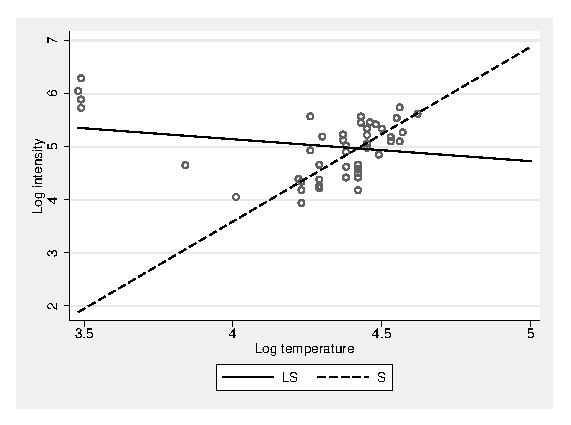
\epsfig{file=eps/4/4}
    \caption{\alert{Caption needed}}
    \label{fig:stars_scatterplot}
\end{figure}

To obtain the \stsc{LS} estimates for the intercept and slope of the regression
of log intensity on log temperature in Stata, without making any difference 
between stars, we can type:

\begin{stlog}
. use CYG-OB1, clear
(Hertzsprung-Russell diagram of star cluster CYG OB1; Rousseeuw/Leroy 1987)
{\smallskip}
. regress log_light log_temp
{\smallskip}
      Source {\VBAR}       SS           df       MS      Number of obs   =        47
\HLI{13}{\PLUS}\HLI{34}   F(1, 45)        =      2.08
       Model {\VBAR}  .664593334         1  .664593334   Prob > F        =    0.1557
    Residual {\VBAR}  14.3463934        45  .318808743   R-squared       =    0.0443
\HLI{13}{\PLUS}\HLI{34}   Adj R-squared   =    0.0230
       Total {\VBAR}  15.0109868        46  .326325799   Root MSE        =    .56463
{\smallskip}
\HLI{13}{\TOPT}\HLI{64}
   log_light {\VBAR}      Coef.   Std. Err.      t    P>|t|     [95\% Conf. Interval]
\HLI{13}{\PLUS}\HLI{64}
    log_temp {\VBAR}  -.4133041   .2862575    -1.44   0.156    -.9898562     .163248
       _cons {\VBAR}   6.793468   1.236516     5.49   0.000     4.302998    9.283939
\HLI{13}{\BOTT}\HLI{64}
{\smallskip}

\end{stlog}

The results of the \stsc{LS} estimation (solid line in
figure~\ref{fig:stars_scatterplot}) indicate that, against intuition, if the
temperature of a star increases, its light intensity decreases in average
(although the effect is not significantly different from zero). If instead of
using a classical estimator we use a robust estimator, the result changes
drastically. For illustrative purposes we will estimate the above model using
\stsc{LTS}, \stsc{LMS}, \stsc{M}, \stsc{GM}, \stsc{S} and \stsc{MM} (with an
efficiency fixed at 95\%) estimators. However, since it has now been widely
accepted that \stsc{S} and \stsc{MM} estimators are preferable to LTS and LMS
because of their higher efficiency and to \stsc{M} and \stsc{GM} estimator
because of their higher robustness with respect to outliers (see above), in the
subsequent examples we will focus exclusively on \stsc{S} and \stsc{MM}
estimates.

\paragraph{LTS}

A robust \stsc{LTS} estimator can be easily fit using the \stcmd{robreg} package 
running the following command:

\begin{stlog}
set seed 1234
{\smallskip}
clear
set obs 1000
{\smallskip}
drawnorm z
gen x=invchi2(1,uniform())
{\smallskip}
{\smallskip}
**** UNCONTAMINATED NORMAL  ******
{\smallskip}
qui sum z, d
local meanN=r(mean)
local medianN=r(p50)
{\smallskip}
local sdN=r(sd)
local iqrN=(r(p75)-r(p25))*0.7413
local skewN=r(skewness)
local kurtN=r(kurtosis)-3
{\smallskip}
centile z, centile(25 50 75)
local qskewN=(r(c_1)+r(c_3)-2*r(c_2))/((r(c_2)-r(c_1))/1.349)
{\smallskip}
qui hl z
local hlN=e(hl)
{\smallskip}
qui qn z
local qnN=e(qn)
{\smallskip}
qui medcouple z, lmc rmc
local mcN=e(mc)
local lmcN=e(lmc)
local rmcN=e(rmc)
{\smallskip}
qui centile z, centile(12.5 25 37.5 62.5 75 87.5)
local lqwN=-(r(c_1)+r(c_3)-2*r(c_2))/(r(c_3)-r(c_1))
local rqwN=(r(c_4)+r(c_6)-2*r(c_5))/(r(c_6)-r(c_4))
{\smallskip}
di in r "Location parameters Normal"
{\smallskip}
di "Mean: " `meanN'
di "Median: " `medianN'
di "Hodges-Lehman: " `hlN'
{\smallskip}
di in r"Scale parameters Normal"
di "Standard deviation: " `sdN'
di "Iqr: " `iqrN'
di "Qn: " `qnN'
{\smallskip}
{\smallskip}
di in r "Skewness parameters Normal"
di "Skewness: " `skewN'
di "Quantile skewness: " `qskewN'
di "Mecouple: " `mcN'
{\smallskip}
di in r "Tail heavyness parameters Normal"
di "Kurtosis: " `kurtN'
di "Quantile right heaviness: " `rqwN'
di "Quantile left heaviness: " `lqwN'
di "Right mecouple: " `rmcN'
di "Left mecouple: " `lmcN'
{\smallskip}
{\smallskip}
**** UNCONTAMINATED CHI2 *****
{\smallskip}
qui sum x, d
local meanCHI2=r(mean)
local medianCHI2=r(p50)
{\smallskip}
local sdCHI2=r(sd)
local iqrCHI2=(r(p75)-r(p25))*0.7413
local skewCHI2=r(skewness)
local kurtCHI2=r(kurtosis)-3
{\smallskip}
centile x, centile(25 50 75)
local qskewCHI2=(r(c_1)+r(c_3)-2*r(c_2))/((r(c_2)-r(c_1))/1.349)
{\smallskip}
qui hl x
local hlCHI2=e(hl)
{\smallskip}
qui qn x
local qnCHI2=e(qn)
{\smallskip}
qui medcouple x, lmc rmc
local mcCHI2=e(mc)
local lmcCHI2=e(lmc)
local rmcCHI2=e(rmc)
{\smallskip}
qui centile x, centile(12.5 25 37.5 62.5 75 87.5)
local lqwCHI2=-(r(c_1)+r(c_3)-2*r(c_2))/(r(c_3)-r(c_1))
local rqwCHI2=(r(c_4)+r(c_6)-2*r(c_5))/(r(c_6)-r(c_4))
{\smallskip}
di in r "Location parameters CHI2"
{\smallskip}
di "Mean: " `meanCHI2'
di "Median: " `medianCHI2'
di "Hodges-Lehman: " `hlCHI2'
{\smallskip}
di in r"Scale parameters CHI2"
di "Standard deviation: " `sdCHI2'
di "Iqr: " `iqrCHI2'
di "Qn: " `qnCHI2'
{\smallskip}
{\smallskip}
di in r "Skewness parameters CHI2"
di "Skewness: " `skewCHI2'
di "Quantile skewness: " `qskewCHI2'
di "Mecouple: " `mcCHI2'
{\smallskip}
di in r "Tail heavyness parameters CHI2"
di "Kurtosis: " `kurtCHI2'
di "Quantile right heaviness: " `rqwCHI2'
di "Quantile left heaviness: " `lqwCHI2'
di "Right mecouple: " `rmcCHI2'
di "Left mecouple: " `lmcCHI2'
{\smallskip}
{\smallskip}
**** CONTAMINATED NORMAL  ******
{\smallskip}
replace z=5 in 1/50
qui sum z, d
local meanNc=r(mean)
local medianNc=r(p50)
{\smallskip}
local sdNc=r(sd)
local iqrNc=(r(p75)-r(p25))*0.7413
local skewNc=r(skewness)
local kurtNc=r(kurtosis)-3
{\smallskip}
centile z, centile(25 50 75)
local qskewNc=(r(c_1)+r(c_3)-2*r(c_2))/((r(c_2)-r(c_1))/1.349)
{\smallskip}
qui hl z
local hlNc=e(hl)
{\smallskip}
qui qn z
local qnNc=e(qn)
{\smallskip}
qui medcouple z, lmc rmc
local mcNc=e(mc)
local lmcNc=e(lmc)
local rmcNc=e(rmc)
{\smallskip}
qui centile z, centile(12.5 25 37.5 62.5 75 87.5)
local lqwNc=-(r(c_1)+r(c_3)-2*r(c_2))/(r(c_3)-r(c_1))
local rqwNc=(r(c_4)+r(c_6)-2*r(c_5))/(r(c_6)-r(c_4))
{\smallskip}
di in r "Location parameters Normal"
{\smallskip}
di "Mean: " `meanNc'
di "Median: " `medianNc'
di "Hodges-Lehman: " `hlNc'
{\smallskip}
di in r"Scale parameters Normal"
di "Standard deviation: " `sdNc'
di "Iqr: " `iqrNc'
di "Qn: " `qnNc'
{\smallskip}
{\smallskip}
di in r "Skewness parameters Normal"
di "Skewness: " `skewNc'
di "Quantile skewness: " `qskewNc'
di "Mecouple: " `mcNc'
{\smallskip}
di in r "Tail heavyness parameters Normal"
di "Kurtosis: " `kurtNc'
di "Quantile right heaviness: " `rqwNc'
di "Quantile left heaviness: " `lqwNc'
di "Right mecouple: " `rmcNc'
di "Left mecouple: " `lmcNc'
{\smallskip}
**** CONTAMINATED CHI2 *****
replace x=invchi2(1,normal(5)) in 1/50
qui sum x, d
local meanCHI2c=r(mean)
local medianCHI2c=r(p50)
{\smallskip}
local sdCHI2c=r(sd)
local iqrCHI2c=(r(p75)-r(p25))*0.7413
local skewCHI2c=r(skewness)
local kurtCHI2c=r(kurtosis)-3
{\smallskip}
centile x, centile(25 50 75)
local qskewCHI2c=(r(c_1)+r(c_3)-2*r(c_2))/((r(c_2)-r(c_1))/1.349)
{\smallskip}
qui hl x
local hlCHI2c=e(hl)
{\smallskip}
qui qn x
local qnCHI2c=e(qn)
{\smallskip}
qui medcouple x, lmc rmc
local mcCHI2c=e(mc)
local lmcCHI2c=e(lmc)
local rmcCHI2c=e(rmc)
{\smallskip}
qui centile x, centile(12.5 25 37.5 62.5 75 87.5)
local lqwCHI2c=-(r(c_1)+r(c_3)-2*r(c_2))/(r(c_3)-r(c_1))
local rqwCHI2c=(r(c_4)+r(c_6)-2*r(c_5))/(r(c_6)-r(c_4))
{\smallskip}
di in r "Location parameters CHI2c"
{\smallskip}
di "Mean: " `meanCHI2c'
di "Median: " `medianCHI2c'
di "Hodges-Lehman: " `hlCHI2c'
{\smallskip}
di in r"Scale parameters CHI2c"
di "Standard deviation: " `sdCHI2c'
di "Iqr: " `iqrCHI2c'
di "Qn: " `qnCHI2c'
{\smallskip}
{\smallskip}
di in r "Skewness parameters CHI2c"
di "Skewness: " `skewCHI2c'
di "Quantile skewness: " `qskewCHI2c'
di "Mecouple: " `mcCHI2c'
{\smallskip}
di in r "Tail heavyness parameters CHI2c"
di "Kurtosis: " `kurtCHI2c'
di "Quantile right heaviness: " `rqwCHI2c'
di "Quantile left heaviness: " `lqwCHI2c'
di "Right mecouple: " `rmcCHI2c'
di "Left mecouple: " `lmcCHI2c'

\end{stlog}

The results from the \stsc{LTS} estimator are
very different from those obtained for the \stsc{LS} estimation. Indeed what we
observe here is that if the log of the temperature of a star increases, its
luminosity will increase as well. In term of size of effect, the \stsc{LTS} estimator
suggests that an increase of 100\% of the temperature is associated to an
increase of the luminosity of approximately 473\%.

\paragraph{LMS}

If instead of the \stsc{LTS} estimator we wish to use the \stsc{LMS} estimator,
we can type:

\begin{stlog}
. robreg lms log_intensity log_temperature
{\smallskip}
enumerating 500 samples (percent completed)
0 \HLI{5} 20 \HLI{6} 40 \HLI{6} 60 \HLI{6} 80 \HLI{5} 100
..................................................
{\smallskip}
LMS regression                                  Number of obs     =         47
                                                  Subsamples      =        500
                                                  Scale estimate  =  .36429398
{\smallskip}
\HLI{14}{\TOPT}\HLI{64}
log_intensity {\VBAR}      Coef.
\HLI{14}{\PLUS}\HLI{64}
log_tempera{\tytilde}e {\VBAR}   3.636368
        _cons {\VBAR}  -11.20184
\HLI{14}{\BOTT}\HLI{64}
{\smallskip}

\end{stlog}

Even if the size of effect seems to be slightly smaller than with \stsc{LTS},
the sign of the relation is the same pointing towards a positive association
between log-temperature and lightness of stars.

\paragraph{M-estimator}

If we use the \stsc{M} estimator (with a Huber
loss function), we do not expect the estimation to resist to outliers. Indeed, 
in the theoretical section it has been shown how this
estimator resists to vertical outliers but not to bad leverage points (i.e.
points outlying in the space of the explanatory variables). As expected, the
\stsc{M} estimation provides results very similar to those of \stsc{LS} and we can conclude
that the estimator breaks down.

The command to run the \stsc{M} estimator is:

\begin{stlog}
. robreg m log_intensity log_temperature
fitting initial LAV estimate ... done
iterating RWLS estimate ........... done
{\smallskip}
M-Regression (95\% efficiency)                   Number of obs     =         47
                                                  Huber k         =  1.3449986
                                                  Scale estimate  =  .63061122
                                                  Robust R2 (w)   =  .04761698
                                                  Robust R2 (rho) =  .03486282
{\smallskip}
\HLI{14}{\TOPT}\HLI{64}
              {\VBAR}               Robust
log_intensity {\VBAR}      Coef.   Std. Err.      z    P>|z|     [95\% Conf. Interval]
\HLI{14}{\PLUS}\HLI{64}
log_tempera{\tytilde}e {\VBAR}  -.4235066   .3992983    -1.06   0.289    -1.206117    .3591036
        _cons {\VBAR}    6.84754   1.758148     3.89   0.000     3.401634    10.29345
\HLI{14}{\BOTT}\HLI{64}
{\smallskip}

\end{stlog}

\paragraph{GM-estimator}

The Generalized \stsc{M} estimate is slightly more complicated to compute than
the \stsc{M} estimate. We first need to estimate the outlyingness of each
individual in the x-dimension, and then downweight leverage points while
estimating the model using an \stsc{M} estimator. In this example, given that
there is a single explanatory variable, the outlyingness in the horizontal
dimension can be measured by centering the data around a robustly estimated
location parameter (e.g. the Hodges-Lehman estimate or the median) and reducing
it using a robustly estimated measure of dispersion (e.g. the Croux and
Rousseeuw $Q_{n}$ estimate). In the case of multiple explanatory variables, the
outlyingness in the space of the explanatory variables will have to be measured
using robust multivariate estimates of location and scatter described in
chapter \alert{XXX}. As far as the down-weighting scheme for outliers is
concerned, several alternatives have been proposed in the literature. In this
example we award a weight equal to zero to any star associated to a leverage
larger than 2.5 and equal to one otherwise. Given that there is one single
explanatory variable, the \stsc{GM} estimator should behave satisfactory.

The commands used for \stsc{GM} estimation are:                                 \todo{To be updated}

\begin{stlog}
. robstat log_temp, statistics(hl qn)
{\smallskip}
Robust Statistics                 Number of obs   =         47
{\smallskip}
\HLI{13}{\TOPT}\HLI{48}
    log_temp {\VBAR}      Coef.   Std. Err.     [95\% Conf. Interval]
\HLI{13}{\PLUS}\HLI{48}
          HL {\VBAR}      4.375          .             .           .
          Qn {\VBAR}   .1553394   .0235479      .1079401    .2027388
\HLI{13}{\BOTT}\HLI{48}
{\smallskip}
. generate leverage = (log_temp - _b[HL])/_b[Qn]
{\smallskip}
. robreg m log_light log_temp if abs(leverage)<=2.5
fitting initial LAV estimate ... done
iterating RWLS estimate ..... done
{\smallskip}
M-Regression (95\% efficiency)                   Number of obs     =         42
                                                  Huber k         =  1.3449986
                                                  Scale estimate  =  .45145187
                                                  Robust R2 (w)   =  .50939875
                                                  Robust R2 (rho) =   .4685587
{\smallskip}
\HLI{13}{\TOPT}\HLI{64}
             {\VBAR}               Robust
   log_light {\VBAR}      Coef.   Std. Err.      z    P>|z|     [95\% Conf. Interval]
\HLI{13}{\PLUS}\HLI{64}
    log_temp {\VBAR}   2.908649   .3751616     7.75   0.000     2.173346    3.643952
       _cons {\VBAR}  -7.875076   1.664063    -4.73   0.000    -11.13658   -4.613572
\HLI{13}{\BOTT}\HLI{64}
{\smallskip}
. drop leverage
{\smallskip}

\end{stlog}


\paragraph{S-estimator}

If we estimate the model using an \stsc{S} estimator, we do not expect to have
large differences with respect to \stsc{LTS}, \stsc{LMS} and \stsc{GM} in terms
of point estimates. However, its higher efficiency makes it theoretically more
appealing. The command to run the \stsc{S} estimator is:

\begin{stlog}
. robreg s log_intensity log_temperature
{\smallskip}
enumerating 50 candidates (percent completed)
0 \HLI{5} 20 \HLI{6} 40 \HLI{6} 60 \HLI{6} 80 \HLI{5} 100
..................................................
{\smallskip}
refining 2 best candidates ... done
{\smallskip}
S-Regression (28.7\% efficiency)                 Number of obs     =         47
                                                  Subsamples      =         50
                                                  Breakdown point =         .5
                                                  Bisquare k      =   1.547645
                                                  Scale estimate  =  .47145696
{\smallskip}
\HLI{14}{\TOPT}\HLI{64}
              {\VBAR}               Robust
log_intensity {\VBAR}      Coef.   Std. Err.      z    P>|z|     [95\% Conf. Interval]
\HLI{14}{\PLUS}\HLI{64}
log_tempera{\tytilde}e {\VBAR}   3.290339    1.64075     2.01   0.045     .0745278    6.506151
        _cons {\VBAR}  -9.570732   7.373867    -1.30   0.194    -24.02325    4.881783
\HLI{14}{\BOTT}\HLI{64}
{\smallskip}

\end{stlog}

The results indicate that if the temperature of a star doubles, its light
intensity increases by approximately 329\%. As stated in the theoretical
section, the gaussian efficiency of the \stsc{S} estimator with a 50\%
breakdown point (and a Tukey biweight loss function) is only 28\%. In order to
increase the efficiency while keeping the breakdown point at 50\%, we can use
\stsc{MM} estimators.

\paragraph{MM-estimator}

It is well-known that even if an \stsc{MM} estimator has a breakdown point of 50\%,
it can be associated to a relatively large bias if its efficiency is set too
high. As explained in Subsection \ref{subsec:Hausman}, a general procedure is
therefore to compare the \stsc{MM} estimate with a given level of efficiency to the
S-estimate, and see if there is a significant difference. If the difference
is small, this means that the bias should not be too big.

We compute here an \stsc{MM} estimator with an efficiency set at 95\%:


\begin{stlog}
. robreg mm log_intensity log_temperature, efficiency(95)
{\smallskip}
Step 1: fitting S-estimate
{\smallskip}
enumerating 50 candidates (percent completed)
0 \HLI{5} 20 \HLI{6} 40 \HLI{6} 60 \HLI{6} 80 \HLI{5} 100
..................................................
{\smallskip}
refining 2 best candidates ... done
{\smallskip}
Step 2: fitting redescending M-estimate
{\smallskip}
iterating RWLS estimate .............. done
{\smallskip}
MM-Regression (95\% efficiency)                  Number of obs     =         47
                                                  Subsamples      =         50
                                                  Breakdown point =         .5
                                                  M-estimate: k   =   4.685045
                                                  S-estimate: k   =   1.547645
                                                  Scale estimate  =  .47145688
                                                  Robust R2 (w)   =  .41883093
                                                  Robust R2 (rho) =  .02050865
{\smallskip}
\HLI{14}{\TOPT}\HLI{64}
              {\VBAR}               Robust
log_intensity {\VBAR}      Coef.   Std. Err.      z    P>|z|     [95\% Conf. Interval]
\HLI{14}{\PLUS}\HLI{64}
log_tempera{\tytilde}e {\VBAR}   2.253165   .7690643     2.93   0.003     .7458263    3.760503
        _cons {\VBAR}  -4.969402   3.410051    -1.46   0.145    -11.65298    1.714175
\HLI{14}{\BOTT}\HLI{64}
{\smallskip}

\end{stlog}

We see that the \stsc{MM} estimation leads to results comparable to the
\stsc{S} estimation in terms of point estimates but is associated to a much
higher efficiency. As explained above, a formal test could have been used but
we leave this for another example. The \stsc{MM} estimated model suggests that
an increase of 100\% of the temperature of a star is associated with an
increase of its luminosity by approximately 225\%. In terms of the quality of
the fit, if we rely on the robust $R^2(w)$ described previously, we see that
the model is pretty good in predicting the luminosity of stars for the vast
majority of the observations. Indeed close to 42\% of the variations in terms
of light intensity for the vast majority of the observations can be explained
by the differences in temperatures.


\subsubsection{Identifying outliers} 

In this second example where the objective is
to unmask outliers, we use a dataset made available by Jeffrey D. Sachs and
Andrew M. Warner in their article \textquotedblleft Natural Resource Abundance
and Economic Growth\textquotedblright\ (1997). In this paper, the authors show
that economies with a high ratio of natural resource exports to GDP in 1970
(the base year) tended to grow slowly during the subsequent 20-year period
1970-1990. In the article the authors aknowledge the existence of outliers and
try to deal with them working with differences in fits.\ More precisely, they
look at how the predicted value for each observation varies when this specific
observation is removed from the sample when fitting the model and compare the
results with the model estimated using all of the observations. They expect to
see big differences in fits for outlying individuals.\ However, if there are
clusters of outliers, atypical individuals will mask one the other and will
most probably not be detected with this technique. The outliers they identify
are Chad, Gabon, Guyana, and Malaysia.

We propose here to use another procedure to identify the outliers. This
procedure is simply based on the examination of the standardized residuals
related to a regression S-estimator.

To identify the outliers, we fist estimate the regression model by running the
command :%

%TCIMACRO{\TeXButton{TeX field}{\tt}}%
%BeginExpansion
%\tt
%EndExpansion
\texttt{robreg s gea7090 lgdpea70 sxp sopen linv7089 rl dtt7090}%
%TCIMACRO{\TeXButton{TeX field}{\it}}%
%BeginExpansion
%\it
%EndExpansion


The results of this S-estimation are presented in Figure ?.%\ref{fig:countries_S_results}.

\textbf{[Insert here S graph from Ch3-Ex-2.do]} \ \newline\ We ask for
the predicted values of the dependent variable by the command:
%TCIMACRO{\TeXButton{TeX field}{\tt}}%
%BeginExpansion
%\tt
%EndExpansion
\texttt{predict yhat}%
%TCIMACRO{\TeXButton{TeX field}{\it}}%
%BeginExpansion
%\it
%EndExpansion
. The robust residuals can then be easily determined using the command:
%TCIMACRO{\TeXButton{TeX field}{\tt}}%
%BeginExpansion
%\tt
%EndExpansion
\texttt{gen res=yhat-gea7090}%
%TCIMACRO{\TeXButton{TeX field}{\it}}%
%BeginExpansion
%\it
%EndExpansion
. They are standardized by dividing them by the scale parameter estimated from
the regression S-estimate:%
%TCIMACRO{\TeXButton{TeX field}{\tt}}%
%BeginExpansion
%\tt
%EndExpansion
\texttt{replace res=res/e(scale)}%
%TCIMACRO{\TeXButton{TeX field}{\it}}%
%BeginExpansion
%\it
%EndExpansion
. We can now plot the standardized residuals and identify those that are
larger or smaller than two given cut-off points corresponding to two specific
quantiles of the normal distribution. We use here the percentiles 2.5 and 97.5
which are respectively equal to -1.96 and 1.96.

We see in Figure ?%\ref{fig:countries_S_standardized_res} 
that, among the four
countries identified as outliers by Sachs and Warner, only Malaysia is still
emerging as outlier when using the S-estimation procedure. On the other hand,
other countries such as Hong Kong, Ecuador or Iran seem to be atypical
countries in the S-regression but were not detected by the original authors.



\textbf{[Insert here S graph from Ch3-Ex-2.do]} \ \newline

\begin{stexample}
\textbf{Testing for the presence of outliers and setting the efficiency for
MM-estimation. }For this example, we again use the dataset relating the
logarithm of the effective temperature at the surface of the star (explanatory
variable $T_{e}$) and the logarithm of its light intensity (dependent variable
$L/L_{0}$). The first question one might raise is: is there a significant
difference between the classical estimate and the robust one? To answer this
question we simply compute an S-estimate using the
%TCIMACRO{\TeXButton{TeX field}{\tt}}%
%BeginExpansion
%\tt
%EndExpansion
\texttt{robreg s}%
%TCIMACRO{\TeXButton{TeX field}{\it} }%
%BeginExpansion
%\it
%EndExpansion
command and use
%TCIMACRO{\TeXButton{TeX field}{\tt}}%
%BeginExpansion
%\tt
%EndExpansion
\texttt{hausman}%
%TCIMACRO{\TeXButton{TeX field}{\it} }%
%BeginExpansion
%\it
%EndExpansion
as an option. This implies that the testing procedure comparing the S-estimate
with the \stsc{LS} estimate (see Subsection \ref{subsec:Hausman}) is implemented.

\textbf{[Insert here S regression from Ch3-Ex-3.do]} \ \newline

The results of the Hausman test (see Figure ?%\ref{fig:stars_Hausman_SvsLS}
)
clearly indicate that the difference between the S-estimate and the
LS-estimate is significant (p-value%
%TCIMACRO{\TEXTsymbol{<}}%
%BeginExpansion
$<$%
%EndExpansion
0.05) and thus that outliers distort the \stsc{LS} estimation. We should therefore
use a robust estimator.

As stated previously S-estimators are very robust against outlier
contamination but are relatively inefficient. MM-estimators on the other hand
are more efficient than S-estimators but might be associated with a large bias
if efficiency is set too high. To choose the level of efficiency to use in
practice we have to apply the testing procedure described in Subsection
\ref{subsec:Hausman} that compares the MM-estimates related to some given
levels of efficiency with respect to an S-estimate. We can then finally set
the efficiency of the MM-estimator at the highest efficiency level that does
not lead to a rejection of the equality between the MM-estimate and the
S-estimate. Doing this in practice is very simple as the testing procedure is
implemented in the
%TCIMACRO{\TeXButton{TeX field}{\tt}}%
%BeginExpansion
%\tt
%EndExpansion
\texttt{robreg mm}%
%TCIMACRO{\TeXButton{TeX field}{\it} }%
%BeginExpansion
%\it
%EndExpansion
command.\ For example, if the
%TCIMACRO{\TeXButton{TeX field}{\tt}}%
%BeginExpansion
%\tt
%EndExpansion
\texttt{robreg mm}%
%TCIMACRO{\TeXButton{TeX field}{\it}}%
%BeginExpansion
%\it
%EndExpansion
\texttt{ }command is run with the efficiency set at 75\% , the
%TCIMACRO{\TeXButton{TeX field}{\tt}}%
%BeginExpansion
%\tt
%EndExpansion
\texttt{hausman}%
%TCIMACRO{\TeXButton{TeX field}{\it} }%
%BeginExpansion
%\it
%EndExpansion
option compares the MM-estimate with 75\% efficiency to the S-estimate
obtained at the first step of the MM-estimation procedure. Similarly, if the
efficiency is set at 85\%, the
%TCIMACRO{\TeXButton{TeX field}{\tt}}%
%BeginExpansion
%\tt
%EndExpansion
\texttt{hausman}%
%TCIMACRO{\TeXButton{TeX field}{\it} }%
%BeginExpansion
%\it
%EndExpansion
option compares the MM-estimate with 85\% efficiency to the S-estimate, and so
on. In this example we control if we can set the efficiency at 75\%, 85\%,
95\%, and 99\%. We obtain the following results:

\begin{itemize}
\item \textbf{MM-estimation with 75\% efficiency:}%

%TCIMACRO{\TeXButton{TeX field}{\tt}}%
%BeginExpansion
%\tt
%EndExpansion
\texttt{robreg mm log\_intensity log\_temperature, hausman efficiency(75)}%
%TCIMACRO{\TeXButton{TeX field}{\it}}%
%BeginExpansion
%\it
%EndExpansion


\textbf{[Insert here MM(75) regression from Ch3-Ex-3.do]} \ \newline

The results of the Hausman test (see Figure ?%\ref{fig:stars_Hausman_SvsMM75}
)
indicate that there is no significant difference between the MM-estimate and
the S-estimate. It would therefore be preferable to work with the MM-estimator
with an efficiency equal to 75\% as it provides results comparable to the
S-estimator in terms of bias but has a much higher efficiency.

\item \textbf{MM-estimation with 85\% efficiency:}%

%TCIMACRO{\TeXButton{TeX field}{\tt}}%
%BeginExpansion
%\tt
%EndExpansion
\texttt{robreg mm log\_intensity log\_temperature, hausman efficiency(85)}%
%TCIMACRO{\TeXButton{TeX field}{\it}}%
%BeginExpansion
%\it
%EndExpansion


\textbf{[Insert here MM(85) regression from Ch3-Ex-3.do]} 

Here again the Hausman test statistics takes a low value which tells us that
there is no significant difference between the MM-estimate and the S-estimate.

\item \textbf{MM-estimation with 95\% efficiency:}%

%TCIMACRO{\TeXButton{TeX field}{\tt}}%
%BeginExpansion
%\tt
%EndExpansion
\texttt{robreg mm log\_intensity log\_temperature, hausman efficiency(95)}%
%TCIMACRO{\TeXButton{TeX field}{\it}}%
%BeginExpansion
%\it
%EndExpansion


\textbf{[Insert here MM(95) regression from Ch3-Ex-3.do]} 

If we set the efficiency of the MM-estimator to 95\%, we still do not observe
any significant difference between the MM-estimate and the S-estimate.

\item \textbf{MM-estimation with 99\% efficieny:}%

%TCIMACRO{\TeXButton{TeX field}{\tt}}%
%BeginExpansion
%\tt
%EndExpansion
\texttt{robreg mm log\_intensity log\_temperature, hausman efficiency(99)}%
%TCIMACRO{\TeXButton{TeX field}{\it}}%
%BeginExpansion
%\it
%EndExpansion


\textbf{[Insert here MM(99) regression from Ch3-Ex-3.do]} 

In the case of an efficiency of the MM-estimator equal to 99\%, the Hausman
test rejects the null hypothesis of equality between the MM-estimate and the
S-estimate, which means that for this very high level of efficiency, the
MM-estimator suffers from a too large bias.

To summarize, it is clear that a classical estimator cannot be used in the
example because the \stsc{LS} estimates are clearly distorted. A robust estimator
should be prefered. We may use an MM-estimator with an efficiency equal to
95\% instead of the less efficient S-estimator since despite the bias from
which the MM-estimator potentially suffers, the MM-estimates of the regression
parameters appear no significantly different from the S-estimates. It is not
recommended to consider a higher level of efficiency for the MM-estimator
(99\%, for instance), since the statistical test indicates that the bias
becomes too big in that case.
\end{itemize}
\end{stexample}

\begin{stexample}
\textbf{Recognizing the type of outliers} For this example, we will use the
very famous auto dataset available from Stata. This dataset contains the price
of a set of cars as well as a series of characteristics. To see if outliers
are present in the dataset, we regress the price on all the available
characteristics and compute the robust standardized residuals. Obviously this
will not allow to recognize the types of outliers. To do so, we will use the
graphical tool of Rousseuw and Van Zomeren (1990).\ The idea here is to use a
scatter plot considering on the vertical dimension the standardized residuals
and on the horizontal dimension the leverage of the observations measured
using the robust Mahalanobis distance (as described in (\ref{eq:leverage})).
For gaussian data it is well known that the standardized residuals are
normally distributed while the robust distances are distributed as a $\chi
_{p}^{2}$ where $p$ is the number of continuous explanatory variables. It is
then natural to compare the standardized residuals and the leverages to some
specific quantiles of the $\mathcal{N}(0,1)$ or $\chi_{p}^{2}$ distributions
in order to detect if an individual has to be considered as an outlier and, if
it is the case, to which type of outlier it corresponds. We decide to choose
here the 2.5th and 97.5th percentiles of the $\mathcal{N}(0,1)$ distribution,
and the 95th percentile of the $\chi_{p}^{2}$ distribution. Those individuals
leading to small robust standardized residuals in absolute value and small
leverages are considered as standard individuals; those giving large
standardized residuals in absolute value and large leverages are defined as
bad leverage points; those that coincide with large standardized residuals in
absolute value but small leverages are considered as vertical outliers and,
finally, those that give small standardized residuals in absolute value but
large leverages are good leverage points. \newline

\textbf{[Insert here MM(95)
regression from Ch3-Ex-4.do]}  \newline\textbf{[Insert here MM(95) graphn from
Ch3-Ex-4.do]}\newline 

Figure ?%\ref{fig:autos_res_leverages} 
clearly shows, for
example, that the Cadillac Seville is a bad leverage point.\ This auto is
indeed associated with a very large positive robust standardized residual and
has a big leverage effect which means that its characteristics in the space of
the explanatory variables are very different from the bulk of the data. On the
other hand, the Cadillac Eldorado, the Lincoln Versaille and some other cars
have a small leverage effect --- their characteristics do not appear as
different from the vast majority of the observations --- but are highly
overpriced given their large positive residuals; these cars are identified as
vertical outliers. Finally some other cars such as the Plymouth Arrow or the
Volkswagen (VW Diesel) \emph{inter alia} are not outliers in terms of prices
but have characteristics very different from the others.\ They are thus good
leverage points. Note that even if these good leverage points do not have
major effect on the estimation of the slope parameter and the constant, they
might affect inference and shrink standard errors.\ It is hence important for
researchers to identify them.
\end{stexample}


\begin{stexample}
\textbf{Dealing with dummies}. For this example, we use the "fertil1.dta" data
set provided provided by Wooldridge (2001) which is a pooled cross section on
more than a thousand U.S. women for the even years between 1972 and 1984.
These data are used to study the relationship between women's education and
fertility. We estimate a model relating the number of children ever born to a
woman (kids) to the years of education, age, age squared, regional dummies,
race dummies, the type of environment in which the women have been reared and
year dummies, using an MS-estimator.\ Given the large number of dummy
variables, it is very likely that the subsampling algorithm described in
Subsection \ref{subsec:MM_estimation} leads to perfectly collinear subsamples.
Using an MS-estimator should tackle the problem.\newline

\textbf{[Insert here MS regression from Ch3-Ex-5.do]}\newline

The results presented in Figure fig:fertil1\_MS\_results clearly point towards
a robust and statistically significant negative relationship between education
and fertility.\ Indeed, each additionnal year of schooling is associated to an
average reduction of fertility (i.e. number of children) equal to 0.19. To
identify the outliers and recognize their type, we again call on the graphical
tool proposed by Rousseuw and Van Zomeren (1990).\ The only difference with
the previous example is that dummy explanatory variables cannot create any
leverage effect and should therefore be treated \ differently from the other
explanatory variables.\ To estimate robust distances, we rely on the Stahel
and Donoho multivariate estimator of location and scatter (this estimator will
be described in details in Chapter ??).\ The latter is a projection based
estimator that allows the pratialling out of dummy variables to calculate
leverage effects. As before we can choose a quantile above which individuals
can be seen as potentially outlying.\ We use here the 0.5th and 99.5th
percentiles of the $\mathcal{N}(0,1)$ distribution as cut-off points for the
robust standardized residuals, and the 99th percentile\ of the chi-square
distribution with $p_{1}$ degrees of freedom, where $p_{1}$ is the number of
continuous explanatory variables, as cut-off point for the robust distances.
In Figure %\ref{fig:fertil1_res_leverages}
, we highlight the women for which
the robust standardized residuals and (or) the robust distances exceed the
cut-off points.

\textbf{[Insert here  graphn from Ch3-Ex-5.do]}\newline

It is evident that individuals such as 565 have more children that one would
expect given their characteristics (which are not quite\textbf{ }different
from the bulk of the data). On the other hand individuals such as 706, 767 or
1063 have characteristics that are very different from the vast majority of
the individuals; however their number of children is in accordance with her
characteristics. Finally individual such as 519, or 490 or 967 have
characteristics that are very different from the others.\ The first one has a
number of children that is much smaller than one would expect according to the
estimated model while the two others have more children than expected.
\end{stexample}

\section{Appendix 1: M-estimators of location and scale}
\label{sec:robreg:appendix1}

The application of the M-estimation approach in the particular case of the
location-scale model (\ref{eq:location_scale_model}) leads to the M-estimators
of location and scale.

\subsection{M-estimator of location}

An M-estimate $\sthat{\mu}_{\stsc{M};\rho}$ of $\mu$ is defined by%

\[
\sthat{\mu}_{\stsc{M};\rho}=\arg\min_{\mu}\sum_{i=1}^{n}\rho\left(
\frac{y_{i}-\mu}{\sthat{\sigma}}\right)
\]
where $\rho\left(  \cdot\right)  $ is a loss function that is positive, even
(such that $\rho\left(  0\right)  =0$) and not decreasing for positive values
$u$, and $\sthat{\sigma}$ is a preliminary robust estimate of $\sigma$ if
this scale parameter is unknown (the MAD, for example). We may also
characterize $\sthat{\mu}_{\stsc{M};\rho}$ as a solution of the following
estimating equation:
\begin{equation}
\sum_{i=1}^{n}\psi\left(  \frac{y_{i}-\mu}{\sthat{\sigma}}\right)  =0,
\label{eq:M_location_equation}%
\end{equation}
where $\psi(u)=\rho^{\prime}(u)$.

Taking $\rho\left(  u\right)  =u^{2}$, we obtain $\psi\left(  u\right)  =2u$
and hence
\[
\sum_{i=1}^{n}\left(  y_{i}-\sthat{\mu}_{\stsc{M};\rho}\right)  =0,
\]
implying that $\sthat{\mu}_{\stsc{M};\rho}=\frac{1}{n}\sum_{i=1}^{n}%
y_{i}=\sthat{\mu}_{\stsc{LS}}$. Taking $\rho\left(  u\right)  =\left\vert
u\right\vert $, we have $\psi(u)=\mathrm{sgn}(u)$ and $\sum_{i=1}%
^{n}\mathrm{sgn}\left(  y_{i}-\sthat{\mu}_{\stsc{M};\rho}\right)  =0$;
this leads to $\sthat{\mu}_{\stsc{M};\rho}=\mathrm{med}\left\{
y_{i}\right\}  =\sthat{\mu}_{\mathrm{L}_{\mathrm{1}}}$.

In general, if $\psi$ is not redescending, the equation
(\ref{eq:M_location_equation}) may be solved using the Newton-Raphson
algorithm with a robust estimate of $\mu$ --- the empirical median
$\mathrm{med}\left\{  y_{i}\right\}  $, for instance --- as initial value for
$\mu$.

The influence function of the functional $T$ associated to the location
M-estimator $\sthat{\mu}_{\stsc{M};\rho}$ under the distribution $F_{0,1}$
of the error term $\nu$ in the location-scale model \ --- recall here that
$F_{0,1}$ is assumed to be symmetric around zero --- takes the form:
\[
\mathrm{IF}\left(  u;T,F_{0,1}\right)  =\frac{\psi(u)}{\mathrm{E}_{F_{0,1}%
}\left[  \psi^{\prime}\left(  \nu\right)  \right]  }.
\]
Consequently, the choice of the function $\rho$, and hence of the function
$\psi$, completely conditions the form of the influence function.

Moreover, it has been proven that an univariate location M-estimator has an
asymptotic breakdown point equal to 50\% whenever the function $\psi$ is
\emph{non decreasing}, bounded and symmetric, and the preliminary estimator of
the scale parameter $\sigma$ is the MAD\footnote{The breakdown point of
$\sthat{\boldsymbol\beta}_{\stsc{M};\rho}$ is actually equal to the
breakdown point of the preliminary estimator of the scale parameter $\sigma$.}
(see \citealp[54]{Huber:2009}). The asymptotic breakdown point is
nul if $\psi$ is unbounded. If $\psi$ is equal to the function $\psi_{\kappa
}^{\stsc{B}}$ and hence is redescending, the breakdown point of
$\sthat{\mu}_{\stsc{M};\rho}$ is strictly smaller than 50\% and depends
upon the breakdown point of the preliminary scale estimator, upon the constant
$\kappa$, but also upon the configuration of the sample (see
\citealp[78]{maronna:etal:2006})\footnote{Note however that it is
possible to prove that, using the MAD as initial scale estimator, the
breakdown point of $\sthat{\mu}_{\stsc{M};\rho_{\kappa}^{\stsc{B}}}$ is
strictly greater than 0.49 in the Gaussian case.}.

\subsection{M-estimator of scale}

A M-estimate $\sthat{\sigma}_{\stsc{M};\rho}$ of the scale parameter
$\sigma$ is defined as the solution of the equation
\begin{equation}
\frac{1}{n}\sum_{i=1}^{n}\rho\left(  \frac{y_{i}-\sthat{\mu}}{\sigma
}\right)  =\delta\label{eq:M_scale_loc_equation}%
\end{equation}
where $\rho\left(  \cdot\right)  $ is a loss function that is positive, even,
not decreasing for positive values and bounded, and $\sthat{\mu}$ is a
preliminary robust estimate of $\mu$ if this location parameter is unknown
(the median, for instance). To ensure the consistency of $\sthat{\sigma
}_{\stsc{M};\rho}$ for $\sigma$, we have to take $\delta=\mathrm{E}%
_{F_{0,1}}\left[  \rho\left(  \nu\right)  \right]  $. An usual choice for the
loss function $\rho$ is the Tukey-Biweight function $\rho_{\kappa}^{B}$
defined by (\ref{eq:Tukey_Biweight_function}).

The M-estimators of scale are translation invariant and scale equivariant. The
influence function of the functional $S$ associated to the scale M-estimator
$\sthat{\sigma}_{\stsc{M};\rho}$ under the distribution $F_{0,1}$ of the
error term $\nu$ of the location-scale model is given by
\[
\mathrm{IF}\left(  u;S,F_{0,1}\right)  =\frac{\rho\left(  u\right)  -\delta
}{\mathrm{E}_{F_{0,1}}\left[  \rho^{\prime}\left(  \nu\right)  \nu\right]  }.
\]
Hence, the choice of a bounded function $\rho$ implies that the influence
function is also bounded. The asymptotic breakdown point of the scale
M-estimator is:
\[
\varepsilon^{\ast}\left(  S,F_{0,1}\right)  =\min\left(  \frac{\delta}%
{\rho\left(  \infty\right)  },1-\frac{\delta}{\rho\left(  \infty\right)
}\right)  ,
\]
which is strictly positive but not always equal to 50\%, even if $\rho$ is bounded.

\begin{stremark}
We may try to jointly estimate $\mu$ and $\sigma$ by solving simultaneously
two equations of the type (\ref{eq:M_location_equation}) and
(\ref{eq:M_scale_loc_equation}) (see, for example, \citealp{Huber:2009}, chapter 6). This complexifies the computations. Moreover, as
explained in \cite{maronna:etal:2006}, it generally provides for
$\sthat{\mu}_{\stsc{M};\rho}$ an asymptotic breakdown point smaller than
50\% --- hence, smaller than the breakdown point attainable by using the MAD
as preliminary estimator of $\sigma$. Consequently, the joint estimation of
$\mu$ and $\sigma$ is not recommended, especially when the scale parameter
$\sigma$ is considered as a nuisance parameter in the location-scale model.
\end{stremark}

\section{Appendix 2: Generalized Method of Moments (GMM) and asymptotic
distributions of regression M-, S- and MM-estimators}

\subsection{GMM-estimation principle}

For simplicity, let us consider immediately the context of the regression
model (\ref{eq:linear_regr_model}). Let $y$ be the scalar dependent variable
and $\stvec{x}=\left(  1,x_{1},\ldots,x_{p}\right)  ^{t}$ be the $\left(
p+1\right)  $-vector of covariates. We assume here that the observations
$\left(  \stvec{x}_{1},y_{1}\right)  ,\ldots,\left(  \stvec{x}_{n}%
,y_{n}\right)  $ are generated by a \emph{stationary}\footnote{A
\emph{stationary} process is a stochastic process whose joint probability
distribution does not change when shifted in time or space. Consequently,
parameters such as the mean and the variance, if they exist, also do not
change over time or position . Hence, the mean and the variance of the process
do not follow trends.} and \emph{ergodic}\footnote{A stochastic process is
said to be \emph{ergodic} if its statistical properties (such as its mean
and variance) can be estimated consistently from a single, sufficiently long
sample (realization) of the process.} process $H$. We also assume, to avoid
too much technicalities, that there is \emph{no autocorrelation}, that is,
that the observations $\left(  \stvec{x}_{i},y_{i}\right)  $, $i = 1, \dots, n$,
are \emph{independent}.\footnote{The interested reader can find very general
results, valid in presence of autocorrelation, in
\cite{Croux:2003}.}

Suppose that our objective is to estimate the functional $\boldsymbol{\theta
}=\boldsymbol{\theta}\left(  H\right)  $ that is implicitly defined by the
equation
\begin{equation}
\mathrm{E}_{H}\left[  \mathbf{m}\left(  y,\stvec{x},\boldsymbol{\theta
}\right)  \right]  =\mathbf{0}, \label{Eq:GMM_moments_conditions}%
\end{equation}
where $\mathbf{m}$ is a known $k$-valued function, and $\mathrm{E}_{H}\left[
\cdot\right]  $ denotes the mathematical expectation with respect to $H$. If
$k$ equals the dimension of the parameter $\boldsymbol{\theta}$ to estimate,
i.e., if the number of moments conditions specified by
(\ref{Eq:GMM_moments_conditions}) co\"{\i}ncides with the dimension of
$\boldsymbol{\theta}$, then the GMM estimation problem is said to be
\emph{exactly-identified}. Note that it is the case in the setting studied
hereafter. The GMM estimator $\sthat{\boldsymbol{\theta}}_{\mathrm{GMM}}$ of
$\boldsymbol{\theta}$ is then simply obtained by solving the sample analogue
of (\ref{Eq:GMM_moments_conditions}), that is,
\begin{equation}
\frac{1}{n}\sum_{i=1}^{n}\mathbf{m}\left(  y_{i},\stvec{x}_{i},\widehat
{\boldsymbol{\theta}}_{\mathrm{GMM}}\right)  =\mathbf{0}.
\label{Eq:GMM_equations}%
\end{equation}


Under regularity conditions detailed in \citet{Hansen:1982}, the GMM
estimator $\sthat{\boldsymbol{\theta}}_{\mathrm{GMM}}$ defined by
(\ref{Eq:GMM_equations}) has a limiting normal distribution: \
\begin{equation}
\sqrt{n}\left(  \sthat{\boldsymbol{\theta}}_{\mathrm{GMM}}%
-\boldsymbol{\theta}\right)  \rightarrow^{d}\mathcal{N}(\mathbf{0}%
,\mathbf{V}), \label{Eq:GMM_estimator_normality}%
\end{equation}
where, in the exactly-identified case,
\begin{equation}
\mathbf{V}=\mathbf{G}^{-1}\boldsymbol{\Omega}\left(  \mathbf{G}^{t}\right)
^{-1}, \label{Eq:GMM_estimator_V}%
\end{equation}
with\footnote{Here and later, we simply write $\mathrm{E}\left[  \cdot\right]
$ for $\mathrm{E}_{H}\left[  \cdot\right]  $.}
\begin{equation}
\mathbf{G}=\mathrm{E}\left[  \frac{\partial\mathbf{m}\left(  y,\stvec{x}%
,\boldsymbol{\theta}\right)  }{\partial\boldsymbol{\theta}^{t}}\right]
\quad\text{and}\quad\boldsymbol{\Omega}=\mathrm{E}\left[  \mathbf{m}\left(
y,\stvec{x},\boldsymbol{\theta}\right)  \mathbf{m}^{t}\left(  y,\stvec{x}%
,\boldsymbol{\theta}\right)  \right]  . \label{Eq:GMM_estimator_G_Omega}%
\end{equation}


\subsection{M-, S- and MM-estimators as GMM-estimators}

Let us first consider the case where we estimate the parameters
$\boldsymbol\beta$ and $\sigma$ simultaneously by an M-estimation procedure.
Let us denote by $\rho\left(  \cdot\right)  $ and $\rho_{0}\left(
\cdot\right)  $ the loss functions used for the M-estimation of
$\boldsymbol\beta$ and $\sigma$, respectively. Then the M-regression
estimator $\sthat{\boldsymbol\beta}_{\stsc{M};\rho}$ and the M-scale
estimator $\sthat{\sigma}_{\rho_{0}}$ are such that
\begin{equation}
\left\{
\begin{array}
[c]{l}%
\dfrac{1}{n}%
%TCIMACRO{\dsum \limits_{i=1}^{n}}%
%BeginExpansion
{\displaystyle\sum\limits_{i=1}^{n}}
%EndExpansion
\psi\left(  \dfrac{y_{i}-\stvec{x}_{i}^{t}\sthat{\boldsymbol\beta%
}_{\stsc{M};\rho}}{\sthat{\sigma}_{\rho_{0}}}\right)  \stvec{x}%
_{i}=\mathbf{0}\\
\dfrac{1}{n}%
%TCIMACRO{\dsum \limits_{i=1}^{n}}%
%BeginExpansion
{\displaystyle\sum\limits_{i=1}^{n}}
%EndExpansion
\rho_{0}\left(  \dfrac{y_{i}-\stvec{x}_{i}^{t}\sthat{\boldsymbol\beta%
}_{\stsc{M};\rho}}{\sthat{\sigma}_{\rho_{0}}}\right)  -\delta=0
\end{array}
\right.  \label{Eq:GMM_equations_M}%
\end{equation}
where $\psi\left(  u\right)  =\rho^{\prime}\left(  u\right)  $, $\delta$ is a
selected constant and, using similar notations as in the previous sections,
$\sthat{\sigma}_{\rho_{0}}=s_{\rho_{0}}\left(  r_{1}\left(  \widehat
{\boldsymbol\beta}_{\stsc{M};\rho}\right)  ,\ldots,r_{n}\left(
\sthat{\boldsymbol\beta}_{\stsc{M};\rho}\right)  \right)  $. This shows
that the M-estimator $\left(  \sthat{\boldsymbol\beta}_{\stsc{M};\rho
}^{t},\sthat{\sigma}_{\rho_{0}}\right)  ^{t}$ is an exactly-identified
GMM-estimator for $\boldsymbol{\theta}=\left(  \boldsymbol\beta^{t}%
,\sigma\right)  ^{t}$, with
\begin{equation}
\mathbf{m}\left(  y,\stvec{x},\boldsymbol{\theta}\right)  =\left(
\begin{array}
[c]{c}%
\psi\left(  \dfrac{y-\stvec{x}^{t}\boldsymbol\beta}{\sigma}\right)
\stvec{x}\\
\rho_{0}\left(  \dfrac{y-\stvec{x}^{t}\boldsymbol\beta}{\sigma}\right)
-\delta
\end{array}
\right)  . \label{Eq:GMM_moment_function_M}%
\end{equation}


S-estimators of regression and scale depend only on a chosen loss function
$\rho_{0}$ and on a constant $\delta$. We have defined the S-regression
estimator $\sthat{\boldsymbol\beta}_{\mathrm{S};\rho_{0}}$ as follows:
\begin{equation}
\sthat{\boldsymbol\beta}_{\mathrm{S};\rho_{0}}=\arg\min_{\boldsymbol{\beta
}}s_{\rho_{0}}\left(  r_{1}\left(  \boldsymbol\beta\right)  ,\ldots
,r_{n}\left(  \boldsymbol\beta\right)  \right)  \label{eq:S_min_rho0}%
\end{equation}
where $s_{\rho_{0}}$ is a measure of dispersion satisfying
\[
\frac{1}{n}\sum_{i=1}^{n}\rho_{0}\left(  \frac{r_{i}\left(  \boldsymbol{\beta
}\right)  }{s_{\rho_{0}}\left(  r_{1}\left(  \boldsymbol\beta\right)
,\ldots,r_{n}\left(  \boldsymbol\beta\right)  \right)  }\right)
-\delta=0\quad\text{for all }\boldsymbol\beta\in\mathbb{R}^{p+1}.
\]
The scale estimator is then simply given by
\[
\sthat{\sigma}_{\rho_{0}}=s_{\rho_{0}}\left(  r_{1}\left(  \widehat
{\boldsymbol\beta}_{\mathrm{S};\rho_{0}}\right)  ,\ldots,r_{n}\left(
\sthat{\boldsymbol\beta}_{\mathrm{S};\rho_{0}}\right)  \right)  .
\]
As previously explained, $\sthat{\boldsymbol\beta}_{\mathrm{S};\rho_{0}}$
and $\sthat{\sigma}_{\rho_{0}}$ satisfy the first order conditions
\begin{equation}
\left\{
\begin{array}
[c]{l}%
\dfrac{1}{n}%
%TCIMACRO{\dsum \limits_{i=1}^{n}}%
%BeginExpansion
{\displaystyle\sum\limits_{i=1}^{n}}
%EndExpansion
\rho_{0}^{\prime}\left(  \dfrac{y_{i}-\stvec{x}_{i}^{t}\widehat
{\boldsymbol\beta}_{\mathrm{S};\rho_{0}}}{\sthat{\sigma}_{\rho_{0}}%
}\right)  \stvec{x}_{i}=\mathbf{0}\\
\dfrac{1}{n}%
%TCIMACRO{\dsum \limits_{i=1}^{n}}%
%BeginExpansion
{\displaystyle\sum\limits_{i=1}^{n}}
%EndExpansion
\rho_{0}\left(  \dfrac{y_{i}-\stvec{x}_{i}^{t}\sthat{\boldsymbol\beta%
}_{\mathrm{S};\rho_{0}}}{\sthat{\sigma}_{\rho_{0}}}\right)  -\delta=0.
\end{array}
\right.  \label{Eq:GMM_equations_S}%
\end{equation}
Note that the equations (\ref{Eq:GMM_equations_S}) are of the same form as
(\ref{Eq:GMM_equations_M}). Hence an S-estimator is first-order equivalent
with an M-estimator where $\rho\left(  \cdot\right)  =\rho_{0}\left(
\cdot\right)  $, and has the same asymptotic distribution (see
\citealp{rousseeuw:yohai:1984}). Note however that the function $\rho_{0}$
defining the S-estimator needs to be bounded to get a positive breakdown point
for the regression estimator. But if $\rho_{0}$ is bounded, $\rho_{0}^{\prime
}$ is redescending and the first set of equations in (\ref{Eq:GMM_equations_S}%
) --- the set of equations involving $\rho_{0}^{\prime}$ --- may have multiple
solutions. Therefore one usually uses (\ref{eq:S_min_rho0}) to compute the
S-estimate but (\ref{Eq:GMM_equations_S}) to determine its asymptotic
distribution. Actually, (\ref{Eq:GMM_equations_S}) implies that $\left(
\sthat{\boldsymbol\beta}_{\mathrm{S};\rho_{0}}^{t},\sthat{\sigma}%
_{\rho_{0}}\right)  ^{t}$ is first-order equivalent with the GMM-estimator for
$\boldsymbol{\theta}=\left(  \boldsymbol\beta^{t},\sigma\right)  ^{t}$,
with
\[
\mathbf{m}\left(  y,\stvec{x},\boldsymbol{\theta}\right)  =\left(
\begin{array}
[c]{c}%
\rho_{0}^{\prime}\left(  \dfrac{y-\stvec{x}^{t}\boldsymbol\beta}{\sigma
}\right)  \stvec{x}\\
\rho_{0}\left(  \dfrac{y-\stvec{x}^{t}\boldsymbol\beta}{\sigma}\right)
-\delta
\end{array}
\right)  .
\]


Let us now focus on MM-estimators of regression. First one needs to compute
S-estimators $\left(  \sthat{\boldsymbol\beta}_{\mathrm{S};\rho_{0}}%
^{t},\sthat{\sigma}_{\rho_{0}}\right)  ^{t}$ for a given function $\rho_{0}$
and a constant $\delta$. Secondly, for a given function $\psi=\rho^{\prime}$,
the MM-estimator of regression solves
\[
\dfrac{1}{n}%
%TCIMACRO{\dsum \limits_{i=1}^{n}}%
%BeginExpansion
{\displaystyle\sum\limits_{i=1}^{n}}
%EndExpansion
\psi\left(  \dfrac{y_{i}-\stvec{x}_{i}^{t}\sthat{\boldsymbol\beta%
}_{\mathrm{MM};\rho_{0},\rho}}{\sthat{\sigma}_{\rho_{0}}}\right)
\stvec{x}_{i}=\mathbf{0}.
\]
Note that $\rho$ needs to be different from $\rho_{0}$, otherwise the
MM-estimator would be equivalent with an S-estimator and share the low
efficiency of the latter. In this MM-estimation procedure, $\widehat
{\boldsymbol\beta}_{\mathrm{MM};\rho_{0},\rho}$, $\sthat{\boldsymbol{\beta
}}_{\mathrm{S};\rho_{0}}$ and $\sthat{\sigma}_{\rho_{0}}$ are such that
\begin{equation}
\left\{
\begin{array}
[c]{l}%
\dfrac{1}{n}%
%TCIMACRO{\dsum \limits_{i=1}^{n}}%
%BeginExpansion
{\displaystyle\sum\limits_{i=1}^{n}}
%EndExpansion
\psi\left(  \dfrac{y_{i}-\stvec{x}_{i}^{t}\sthat{\boldsymbol\beta%
}_{\mathrm{MM};\rho_{0},\rho}}{\sthat{\sigma}_{\rho_{0}}}\right)
\stvec{x}_{i}=\mathbf{0}\\
\dfrac{1}{n}%
%TCIMACRO{\dsum \limits_{i=1}^{n}}%
%BeginExpansion
{\displaystyle\sum\limits_{i=1}^{n}}
%EndExpansion
\rho_{0}^{\prime}\left(  \dfrac{y_{i}-\stvec{x}_{i}^{t}\widehat
{\boldsymbol\beta}_{\mathrm{S};\rho_{0}}}{\sthat{\sigma}_{\rho_{0}}%
}\right)  \stvec{x}_{i}=\mathbf{0}\\
\dfrac{1}{n}%
%TCIMACRO{\dsum \limits_{i=1}^{n}}%
%BeginExpansion
{\displaystyle\sum\limits_{i=1}^{n}}
%EndExpansion
\rho_{0}\left(  \dfrac{y_{i}-\stvec{x}_{i}^{t}\sthat{\boldsymbol\beta%
}_{\mathrm{S};\rho_{0}}}{\sthat{\sigma}_{\rho_{0}}}\right)  -\delta=0.
\end{array}
\right.  \label{Eq:GMM_equations_MM}%
\end{equation}
Defining $\boldsymbol{\theta}=(\boldsymbol\beta^{t},\boldsymbol\beta%
_{0}^{t},\sigma)^{t}$, where the first parameter $\boldsymbol\beta$ will be
estimated by $\sthat{\boldsymbol\beta}_{\mathrm{MM};\rho_{0},\rho}$ and
the latter two by $\sthat{\boldsymbol\beta}_{\mathrm{S};\rho_{0}}$ and
$\sthat{\sigma}_{\rho_{0}}$, equations (\ref{Eq:GMM_equations_MM}) show that
$(\sthat{\boldsymbol\beta}_{\mathrm{MM};\rho_{0},\rho}^{t},\widehat
{\boldsymbol\beta}_{\mathrm{S};\rho_{0}}^{t},\sthat{\sigma}_{\rho_{0}%
})^{t}$ is first-order equivalent with the GMM-estimator for
$\boldsymbol{\theta}$, with
\[
\mathbf{m}\left(  y,\stvec{x},\boldsymbol{\theta}\right)  =\left(
\begin{array}
[c]{c}%
\psi\left(  \dfrac{y-\stvec{x}^{t}\boldsymbol\beta}{\sigma}\right)
\stvec{x}\\
\rho_{0}^{\prime}\left(  \dfrac{y-\stvec{x}^{t}\boldsymbol\beta_{0}}%
{\sigma}\right)  \stvec{x}\\
\rho_{0}\left(  \dfrac{y-\stvec{x}^{t}\boldsymbol\beta_{0}}{\sigma}\right)
-\delta
\end{array}
\right)  .
\]
Using the generic notations $u_{0}=\frac{y-\stvec{x}^{t}\boldsymbol{\beta
}_{0}}{\sigma}$ and $u=\frac{y-\stvec{x}^{t}\boldsymbol\beta}{\sigma}$, the
moment function $\mathbf{m}\left(  y,\stvec{x},\boldsymbol{\theta}\right)  $
takes the simpler form
\[
\mathbf{m}\left(  y,\stvec{x},\boldsymbol{\theta}\right)  =\left(
\begin{array}
[c]{c}%
\psi\left(  u\right)  \stvec{x}\\
\rho_{0}^{\prime}\left(  u_{0}\right)  \stvec{x}\\
\rho_{0}\left(  u_{0}\right)  -\delta
\end{array}
\right)  ,
\]
or still more shortly,
\begin{equation}
\mathbf{m}\left(  y,\stvec{x},\boldsymbol{\theta}\right)  =\left(
\begin{array}
[c]{c}%
\psi\stvec{x}\\
\rho_{0}^{\prime}\stvec{x}\\
\rho_{0}-\delta
\end{array}
\right)  , \label{Eq:GMM_moment_function_MM}%
\end{equation}
if we simply replace $\psi\left(  u\right)  $ by $\psi$, $\rho_{0}\left(
u_{0}\right)  $ by $\rho_{0}$, and $\rho_{0}^{\prime}\left(  u_{0}\right)  $
by $\rho_{0}^{\prime}$. This compact notation for the moment function will be
more practice to use in the sequel.

\subsection{Asymptotic variance matrix of an MM-estimator}

\subsubsection{If the observations $\left(  \stvec{x}_{i},y_{i}\right)  $,
$i = 1, \dots, n$, are generated by a stationary and ergodic process, and are
independent (Assumption A1)}

The first-order equivalence of $(\sthat{\boldsymbol\beta}_{\mathrm{MM}%
;\rho_{0},\rho}^{t},\sthat{\boldsymbol\beta}_{\mathrm{S};\rho_{0}}%
^{t},\sthat{\sigma}_{\rho_{0}})^{t}$ with a GMM-estimator for
$\boldsymbol{\theta}=(\boldsymbol\beta^{t},\boldsymbol\beta_{0}^{t}%
,\sigma)^{t}$ allows us to conclude that, if the observations $\left(
\stvec{x}_{1},y_{1}\right)  ,\ldots,\left(  \stvec{x}_{n},y_{n}\right)  $
are generated by a \emph{stationary} and \emph{ergodic} process, and are
\emph{independent} (Assumption A1)\footnote{This Assumption A1 coincides
with Assumption A in Section \ref{subsec:asymptotic_distr_M_S_MM_estimators}.
We add here an number to the letter “A” in order to clearly distinguish the
various assumptions we will consider in the sequel of this appendix.},
\[
\sqrt{n}\left(  \left(
\begin{array}
[c]{c}%
\sthat{\boldsymbol\beta}_{\mathrm{MM};\rho_{0},\rho}\\
\sthat{\boldsymbol\beta}_{\mathrm{S};\rho_{0}}\\
\sthat{\sigma}_{\rho_{0}}%
\end{array}
\right)  -\left(
\begin{array}
[c]{c}%
\boldsymbol\beta\\
\boldsymbol\beta_{0}\\
\sigma
\end{array}
\right)  \right)  \rightarrow^{d}\mathcal{N}(\mathbf{0},\mathbf{V}%
_{\mathrm{MM}})
\]
where
\[
\mathbf{V}_{\mathrm{MM}}=\mathbf{G}_{\mathrm{MM}}^{-1}\boldsymbol{\Omega
}_{\mathrm{MM}}\left(  \mathbf{G}_{\mathrm{MM}}^{t}\right)  ^{-1},
\]
with the matrices $\mathbf{G}_{\mathrm{MM}}$ and $\boldsymbol{\Omega
}_{\mathrm{MM}}$ obtained by applying relations
(\ref{Eq:GMM_estimator_G_Omega}) to the moment function
(\ref{Eq:GMM_moment_function_MM}):
\[
\mathbf{G}_{\mathrm{MM}}=-\frac{1}{\sigma}\mathrm{E}\left(
\begin{array}
[c]{ccc}%
\psi^{\prime}\mathbf{xx}^{t} & \mathbf{0} & \psi^{\prime}u\stvec{x}\\
\mathbf{0} & \rho_{0}^{\prime\prime}\mathbf{xx}^{t} & \rho_{0}^{\prime\prime
}u_{0}\stvec{x}\\
\mathbf{0} & \mathbf{0} & \rho_{0}^{\prime}u_{0}%
\end{array}
\right)
\]
and
\[
\boldsymbol{\Omega}_{\mathrm{MM}}=\mathrm{E}\left(
\begin{array}
[c]{ccc}%
\psi^{2}\mathbf{xx}^{t} & \psi\rho_{0}^{\prime}\mathbf{xx}^{t} & \psi\rho
_{0}\stvec{x}\\
\psi\rho_{0}^{\prime}\mathbf{xx}^{t} & \left(  \rho_{0}^{\prime}\right)
^{2}\mathbf{xx}^{t} & \rho_{0}\rho_{0}^{\prime}\stvec{x}\\
\psi\rho_{0}\stvec{x}^{t} & \rho_{0}\rho_{0}^{\prime}\stvec{x}^{t} &
\rho_{0}^{2}-\delta^{2}%
\end{array}
\right)  .
\]
In particular, this result establishes the consistency of the MM-regression
estimator $\sthat{\boldsymbol\beta}_{\mathrm{MM};\rho_{0},\rho}$.
Moreover, using the upper left $\left(  p+1\right)  \times(p+1)$ submatrice of
$\mathbf{V}_{\mathrm{MM}}$, we obtain that the asymptotic variance of
$\sthat{\boldsymbol\beta}_{\mathrm{MM};\rho_{0},\rho}$ is equal to
\begin{align*}
\mathrm{Avar}_{1}\left(  \sthat{\boldsymbol\beta}_{\mathrm{MM};\rho
_{0},\rho}\right)   &  =\frac{1}{n}[\mathbf{A}\mathrm{E}\left(  \psi
^{2}\mathbf{xx}^{t}\right)  \mathbf{A}-\mathbf{a}\mathrm{E}\left(  \psi
\rho_{0}\stvec{x}^{t}\right)  \mathbf{A}\\
&  \,\ \ \ \ \ \ \ \ \ -\mathbf{A}\mathrm{E}\left(  \psi\rho_{0}%
\stvec{x}\right)  \mathbf{a}^{t}+\mathrm{E}\left(  \rho_{0}^{2}-\delta
^{2}\right)  \mathbf{aa}^{t}],
\end{align*}
where
\[
\mathbf{A}=\sigma\left[  \mathrm{E}\left(  \psi^{\prime}\mathbf{xx}%
^{t}\right)  \right]  ^{-1}\quad\text{and\quad}\mathbf{a}=\mathbf{A}%
\frac{\mathrm{E}\left(  \psi^{\prime}u\stvec{x}\right)  }{\mathrm{E}\left(
\rho_{0}^{\prime}u_{0}\right)  }.
\]
This expression of $\mathrm{Avar}_{1}\left(  \sthat{\boldsymbol\beta%
}_{\mathrm{MM};\rho_{0},\rho}\right)  $ is then estimated by its empirical
counterpart $\sthat{\mathrm{Avar}}_{1}\left(  \sthat{\boldsymbol\beta%
}_{\mathrm{MM};\rho_{0},\rho}\right)  $, by applying the following two rules:

\begin{enumerate}
\item Replace, in $u$ and $u_{0}$, the parameters $\boldsymbol\beta$,
$\boldsymbol\beta_{0}$ and $\sigma$ by the estimates $\widehat
{\boldsymbol\beta}_{\mathrm{MM};\rho_{0},\rho}$, $\sthat{\boldsymbol{\beta
}}_{\mathrm{S};\rho_{0}}$ and $\sthat{\sigma}_{\rho_{0}}$.

\item Replace $\mathrm{E}\left(  \cdot\right)  $ by $\frac{1}{n}\sum_{i=1}%
^{n}\left(  \cdot\right)  $.
\end{enumerate}

For example, the first term of $\sthat{\mathrm{Avar}}_{1}\left(
\sthat{\boldsymbol\beta}_{\mathrm{MM};\rho_{0},\rho}\right)  $ is given
by
\[
\frac{1}{n}\left[  \sthat{\mathbf{A}}\left(  \frac{1}{n}\sum_{i=1}%
^{n}\left[  \psi\left(  \frac{y_{i}-\stvec{x}_{i}^{t}\widehat
{\boldsymbol\beta}_{\mathrm{MM};\rho_{0},\rho}}{\sthat{\sigma}_{\rho_{0}}%
}\right)  \right]  ^{2}\stvec{x}_{i}\stvec{x}_{i}^{t}\right)  \widehat
{\mathbf{A}}\right]
\]
with
\[
\sthat{\mathbf{A}}=\sthat{\sigma}_{\rho_{0}}\left[  \frac{1}{n}\sum
_{i=1}^{n}\psi^{\prime}\left(  \frac{y_{i}-\stvec{x}_{i}^{t}\widehat
{\boldsymbol\beta}_{\mathrm{MM};\rho_{0},\rho}}{\sthat{\sigma}_{\rho_{0}}%
}\right)  \stvec{x}_{i}\stvec{x}_{i}^{t}\right]  ^{-1}.
\]


Using standard asymptotic arguments, it can be shown that $\widehat
{\mathrm{Avar}}_{1}\left(  \sthat{\boldsymbol\beta}_{\mathrm{MM};\rho
_{0},\rho}\right)  $ is a consistent estimate of $\mathrm{Avar}_{1}\left(
\sthat{\boldsymbol\beta}_{\mathrm{MM};\rho_{0},\rho}\right)  $. From
$\sthat{\mathrm{Avar}}_{1}\left(  \sthat{\boldsymbol\beta}%
_{\mathrm{MM};\rho_{0},\rho}\right)  $, standard errors for the regression
coefficients are obtained in the usual way: for $j=0,1,\ldots,p$,
\[
\sthat{\mathrm{se}}\left(  \left[  \sthat{\boldsymbol\beta}%
_{\mathrm{MM};\rho_{0},\rho}\right]  _{j}\right)  =\sqrt{\left[
\sthat{\mathrm{Avar}}_{1}\left(  \sthat{\boldsymbol\beta}_{\mathrm{MM}%
;\rho_{0},\rho}\right)  \right]  _{jj}}.
\]


Moreover, the estimate $\sthat{\mathrm{Avar}}_{1}\left(  \widehat
{\boldsymbol\beta}_{\mathrm{MM};\rho_{0},\rho}\right)  $ of the asymptotic
variance $\mathrm{Avar}_{1}\left(  \sthat{\boldsymbol\beta}_{\mathrm{MM}%
;\rho_{0},\rho}\right)  $ is robust with respect to bad leverage points and
vertical outliers. Indeed, if there are observations yielding large residuals
with respect to the robust MM-fit, then $\psi\left(  \frac{y_{i}%
-\stvec{x}_{i}^{t}\sthat{\boldsymbol\beta}_{\mathrm{MM};\rho_{0},\rho}%
}{\sthat{\sigma}_{\rho_{0}}}\right)  $ has a small value when $\psi$ is a
redescending function\footnote{Recall that, if $\psi$ is redescending, it has
the property to be equal to zero for large arguments.}. Hence, if there are
bad leverage points in the sample, then their $\stvec{x}_{i}$-value is large,
but at the same time $\psi\left(  \frac{y_{i}-\stvec{x}_{i}^{t}%
\sthat{\boldsymbol\beta}_{\mathrm{MM};\rho_{0},\rho}}{\sthat{\sigma
}_{\rho_{0}}}\right)  $ will be zero. This explains intuitively why vertical
outliers and bad leverage points have only a limited influence on the estimate
$\sthat{\mathrm{Avar}}_{1}\left(  \sthat{\boldsymbol\beta}%
_{\mathrm{MM};\rho_{0},\rho}\right)  $.

\subsubsection{In absence of heteroskedasticity (Assumption A2)}

A simplification of the asymptotic variance of $\sthat{\boldsymbol\beta%
}_{\mathrm{MM};\rho_{0},\rho}$ occurs when, in addition to Assumption A1, we
also assume that there is \emph{no heteroskedasticity}, i.e., we assume that
the processes $\stvec{x}_{i}$ and $\left(  u_{i},u_{0i}\right)  $ are
independent (Assumption A2). In that case, the asymptotic variance of
$\sthat{\boldsymbol\beta}_{\mathrm{MM};\rho_{0},\rho}$ becomes
\begin{align*}
\mathrm{Avar}_{12}\left(  \sthat{\boldsymbol\beta}_{\mathrm{MM};\rho
_{0},\rho}\right)   &  =\frac{1}{n}[\mathrm{E}\left(  \psi^{2}\right)
\mathbf{A}_{2}\mathrm{E}\left(  \mathbf{xx}^{t}\right)  \mathbf{A}%
_{2}-\mathrm{E}\left(  \psi\rho_{0}\right)  \mathbf{a}_{2}\mathrm{E}\left(
\stvec{x}^{t}\right)  \mathbf{A}_{2}\\
&  \hspace{0in}\hspace{1cm}-\mathrm{E}\left(  \psi\rho_{0}\right)
\mathbf{A}_{2}\mathrm{E}\left(  \stvec{x}\right)  \mathbf{a}_{2}%
^{t}+\mathrm{E}\left(  \rho_{0}^{2}-\delta^{2}\right)  \mathbf{a}%
_{2}\mathbf{a}_{2}^{t}],
\end{align*}
where
\[
\mathbf{A}_{2}=\sigma\frac{\left[  \mathrm{E}\left(  \mathbf{xx}^{t}\right)
\right]  ^{-1}}{\mathrm{E}\left(  \psi^{\prime}\right)  }\quad\text{and\quad
}\mathbf{a}_{2}=\mathbf{A}_{2}\frac{\mathrm{E}\left(  \psi^{\prime}u\right)
\mathrm{E}\left(  \stvec{x}\right)  }{\mathrm{E}\left(  \rho_{0}^{\prime
}u_{0}\right)  }.
\]
Taking the empirical counterpart yields $\sthat{\mathrm{Avar}}_{12}\left(
\sthat{\boldsymbol\beta}_{\mathrm{MM};\rho_{0},\rho}\right)  $. However,
Croux \textit{et al.} (2003) do advise against the use of this variance matrix
estimator in practice, even when assumptions A1 and A2 holds. The reason is
that this estimator will not be robust with respect to (good and bad) leverage
points. Indeed, $\sthat{\mathbf{A}}_{2}$, for example, is proportional to
the inverse of an empirical second moment matrix of the observations
$\stvec{x}_{i}$. Leverage points are outlying in the covariates' space, and
will then have a strong influence on $\sthat{\mathbf{A}}_{2}$. This can even
lead $\sthat{\mathrm{Avar}}_{12}\left(  \sthat{\boldsymbol\beta%
}_{\mathrm{MM};\rho_{0},\rho}\right)  $ to break down, where breakdown of a
variance matrix estimator means that the latter has a determinant close to
zero or enormously large.

\subsubsection{If the distribution of the error terms is symmetric around zero (Assumption A3)}

A condition often imposed in the literature is that the distribution of
$u_{i}=\frac{y_{i}-\stvec{x}_{i}^{t}\boldsymbol\beta}{\sigma}$, given
$\stvec{x}_{i}$, is symmetric (Assumption A3). If this condition is met, the
regression parameter estimator and the estimator of residual scale are
asymptotically independent, and the different expressions simplify
considerably, due to the fact that $\mathbf{a}=\mathbf{0}$.

Under Assumptions A1 and A3, the asymptotic variance of $\widehat
{\boldsymbol\beta}_{\mathrm{MM};\rho_{0},\rho}$ becomes
\begin{align*}
\mathrm{Avar}_{13}\left(  \sthat{\boldsymbol\beta}_{\mathrm{MM};\rho
_{0},\rho}\right)   &  =\frac{1}{n}\mathbf{A}\mathrm{E}\left(  \psi
^{2}\mathbf{xx}^{t}\right)  \mathbf{A}\\
&  =\frac{\sigma^{2}}{n}\left[  \mathrm{E}\left(  \psi^{\prime}\mathbf{xx}%
^{t}\right)  \right]  ^{-1}\mathrm{E}\left(  \psi^{2}\mathbf{xx}^{t}\right)
\left[  \mathrm{E}\left(  \psi^{\prime}\mathbf{xx}^{t}\right)  \right]  ^{-1}.
\end{align*}
The empirical counterpart of the latter expression, $\sthat{\mathrm{Avar}%
}_{13}\left(  \sthat{\boldsymbol\beta}_{\mathrm{MM};\rho_{0},\rho}\right)
$, is an estimate of the asymptotic variance of $\sthat{\boldsymbol\beta%
}_{\mathrm{MM};\rho_{0},\rho}$ that is robust against vertical outliers and
bad leverage points. But it relies on symmetry of the errors distribution, a
quite strong assumption. A simulation study in \cite{Croux:2003} shows that, even when symmetry is present, there is no gain in using
$\sthat{\mathrm{Avar}}_{13}$ compared to $\sthat{\mathrm{Avar}}_{1}$: the
authors of \cite{Croux:2003} then recommend to use
$\sthat{\mathrm{Avar}}_{1}$ in any case.

When all of Assumptions A1, A2 and A3 hold, then $\sthat{\boldsymbol\beta%
}_{\mathrm{MM};\rho_{0},\rho}$ has asymptotic variance
\[
\mathrm{Avar}_{123}\left(  \sthat{\boldsymbol\beta}_{\mathrm{MM};\rho
_{0},\rho}\right)  =\frac{\sigma^{2}}{n}\frac{\mathrm{E}\left(  \psi
^{2}\right)  }{\left[  \mathrm{E}\left(  \psi^{\prime}\right)  \right]  ^{2}%
}\left[  \mathrm{E}\left(  \mathbf{xx}^{t}\right)  \right]  ^{-1}.
\]
This corresponds to the expression for the variance of the MM-regression
estimator that was derived in \cite{yohai:1987}. The empirical counterpart
$\sthat{\mathrm{Avar}}_{123}\left(  \sthat{\boldsymbol\beta%
}_{\mathrm{MM};\rho_{0},\rho}\right)  $ is an estimate of this asymptotic
variance that, as $\sthat{\mathrm{Avar}}_{12}\left(  \widehat
{\boldsymbol\beta}_{\mathrm{MM};\rho_{0},\rho}\right)  $, lacks robustness
with respect to leverage points.

\subsection{Asymptotic variance matrix of an S-estimator}

If Assumption A1 holds, the asymptotic variance matrix of $\widehat
{\boldsymbol\beta}_{\mathrm{S};\rho_{0}}$ is simply derived from the central
$(p+1)\times(p+1)$ submatrice of $\mathbf{V}_{\mathrm{MM}}$ (cf.
(\ref{eq:V_MM}), (\ref{eq:G_MM}) and (\ref{eq:Omega_MM})):
\begin{align*}
\mathrm{Avar}_{1}\left(  \sthat{\boldsymbol\beta}_{\mathrm{S};\rho_{0}%
}\right)   &  =\frac{1}{n}[\mathbf{A}_{\mathrm{S}}\mathrm{E}\left(  \left(
\rho_{0}^{\prime}\right)  ^{2}\mathbf{xx}^{t}\right)  \mathbf{A}_{\mathrm{S}%
}-\mathbf{a}_{\mathrm{S}}\mathrm{E}\left(  \rho_{0}\rho_{0}^{\prime}%
\stvec{x}^{t}\right)  \mathbf{A}_{\mathrm{S}}\\
&  \hspace{1cm}-\mathbf{A}_{\mathrm{S}}\mathrm{E}\left(  \rho_{0}\rho
_{0}^{\prime}\stvec{x}\right)  \mathbf{a}_{\mathrm{S}}^{t}+\mathrm{E}\left(
\rho_{0}^{2}-\delta^{2}\right)  \mathbf{a}_{\mathrm{S}}\mathbf{a}_{\mathrm{S}%
}^{t}],
\end{align*}
where
\[
\mathbf{A}_{\mathrm{S}}=\sigma\left[  \mathrm{E}\left(  \rho_{0}^{\prime
\prime}\mathbf{xx}^{t}\right)  \right]  ^{-1}\quad\text{and\quad}%
\mathbf{a}_{\mathrm{S}}=\mathbf{A}_{\mathrm{S}}\frac{\mathrm{E}\left(
\rho_{0}^{\prime\prime}u_{0}\stvec{x}\right)  }{\mathrm{E}\left(  \rho
_{0}^{\prime}u_{0}\right)  }.
\]
If, in addition, A2 holds, then the asymptotic variance matrix of
$\sthat{\boldsymbol\beta}_{\mathrm{S};\rho_{0}}$ takes the form
\begin{align*}
\mathrm{Avar}_{12}\left(  \sthat{\boldsymbol\beta}_{\mathrm{S};\rho_{0}%
}\right)   &  =\frac{\sigma^{2}}{n}\frac{\mathrm{E}\left(  \left(  \rho
_{0}^{\prime}\right)  ^{2}\right)  }{\left[  \mathrm{E}\left(  \rho
_{0}^{\prime\prime}\right)  \right]  ^{2}}\left[  \mathrm{E}\left(
\mathbf{xx}^{t}\right)  \right]  ^{-1}+\frac{\sigma^{2}}{n}\frac
{\mathrm{E}\left(  \rho_{0}^{\prime\prime}u_{0}\right)  }{\left[
\mathrm{E}\left(  \rho_{0}^{\prime\prime}\right)  \right]  ^{2}\mathrm{E}%
\left(  \rho_{0}^{\prime}u_{0}\right)  }\\
&  \qquad\times\left\{  \frac{\mathrm{E}\left(  \rho_{0}^{\prime\prime}%
u_{0}\right)  \mathrm{E}\left(  \rho_{0}^{2}-\delta^{2}\right)  }%
{\mathrm{E}\left(  \rho_{0}^{\prime}u_{0}\right)  }-2\mathrm{E}\left(
\rho_{0}\rho_{0}^{\prime}\right)  \right\} \\
&  \qquad\times\left[  \mathrm{E}\left(  \mathbf{xx}^{t}\right)  \right]
^{-1}\mathrm{E}\left(  \stvec{x}\right)  \mathrm{E}\left(  \stvec{x}%
^{t}\right)  \left[  \mathrm{E}\left(  \mathbf{xx}^{t}\right)  \right]  ^{-1}.
\end{align*}
Under A3, the expressions are the same as those for the MM-estimator, with
$\psi$ replaced by $\rho_{0}^{\prime}$.

\subsection{Asymptotic variance matrix of an M-estimator}

Here the expressions are less explicit. Under Assumption A1, the asymptotic
variance of $\sthat{\boldsymbol\beta}_{\stsc{M};,\rho}$ is derived from
the upper left $(p+1)\times(p+1)$ block of $\mathbf{G}_{\stsc{M}}%
^{-1}\boldsymbol{\Omega}_{\stsc{M}}\left(  \mathbf{G}_{\stsc{M}}%
^{t}\right)  ^{-1}$ where
\[
\mathbf{G}_{\stsc{M}}=\mathrm{E}\left[  \frac{\partial\mathbf{m}\left(
y,\stvec{x},\boldsymbol{\theta}\right)  }{\partial\boldsymbol{\theta}^{t}%
}\right]  \quad\text{and}\quad\boldsymbol{\Omega}_{\stsc{M}}=\mathrm{E}%
\left[  \mathbf{m}\left(  y,\stvec{x},\boldsymbol{\theta}\right)
\mathbf{m}^{t}\left(  y,\stvec{x},\boldsymbol{\theta}\right)  \right]  ,
\]
with $\mathbf{m}\left(  y,\stvec{x},\boldsymbol{\theta}\right)  $ given by
(\ref{Eq:GMM_moment_function_M}). Defining $u=\frac{y-\stvec{x}%
^{t}\boldsymbol\beta}{\sigma}$, and denoting shortly $\rho^{\prime}%
(u)=\psi(u)$ and $\rho_{0}(u)$ by $\psi$ and $\rho_{0}$, respectively, we
have
\[
\mathbf{G}_{\stsc{M}}=-\frac{1}{\sigma}\mathrm{E}\left(
\begin{array}
[c]{cc}%
\psi^{\prime}\mathbf{xx}^{t} & \psi^{\prime}u\stvec{x}\\
\rho_{0}^{\prime}\stvec{x}^{t} & \rho_{0}^{\prime}u
\end{array}
\right)
\]
and
\[
\boldsymbol{\Omega}_{\stsc{M}}=\mathrm{E}\left(
\begin{array}
[c]{cc}%
\psi^{2}\mathbf{xx}^{t} & \psi\rho_{0}\stvec{x}\\
\psi\rho_{0}\stvec{x}^{t} & \rho_{0}^{2}-\delta^{2}%
\end{array}
\right)  .
\]


If in addition Assumption A2 holds, then
\[
\mathbf{G}_{\stsc{M}}=-\frac{1}{\sigma}\left(
\begin{array}
[c]{cc}%
\mathrm{E}\left(  \psi^{\prime}\right)  \mathrm{E}\left(  \mathbf{xx}%
^{t}\right)  & \mathrm{E}\left(  \psi^{\prime}u\right)  \mathrm{E}\left(
\stvec{x}\right) \\
\mathrm{E}\left(  \rho_{0}^{\prime}\right)  \mathrm{E}\left(  \stvec{x}%
^{t}\right)  & \mathrm{E}\left(  \rho_{0}^{\prime}u\right)
\end{array}
\right)
\]
and
\[
\boldsymbol{\Omega}_{\stsc{M}}=\left(
\begin{array}
[c]{cc}%
\mathrm{E}\left(  \psi^{2}\right)  \mathrm{E}\left(  \mathbf{xx}^{t}\right)  &
\mathrm{E}\left(  \psi\rho_{0}\right)  \mathrm{E}\left(  \stvec{x}\right) \\
\mathrm{E}\left(  \psi\rho_{0}\right)  \mathrm{E}\left(  \stvec{x}^{t}\right)
& \mathrm{E}\left(  \rho_{0}^{2}\right)  -\delta^{2}%
\end{array}
\right)  .
\]
Under Assumption A3, the expressions of $\mathrm{Avar}_{13}\left(
\sthat{\boldsymbol\beta}_{\stsc{M};\rho}\right)  $ and $\mathrm{Avar}%
_{123}\left(  \sthat{\boldsymbol\beta}_{\stsc{M};\rho}\right)  $ are
exactly similar to those for the MM-estimator.

% \begin{thebibliography}{99}

% \bibitem {Anderson (1984)}Anderson, T.W. (1984), \textit{An Introduction to
% Multivariate Statistical Analysis} (second ed.), John Wiley \& Sons.

% \bibitem {Andrews (1974)}Andrews, D.F. (1974), A Robust Method for Multiple
% Linear Regression, \textit{Technometrics}, \textbf{16}, 523-531.

% \bibitem {Blasnick (1998)}???

% \bibitem {Bramati.Croux (2007)}Bramati, M. C. and Croux, C. (2007), Robust
% Estimators for the Fixed Effects Panel Data Model, \textit{Econometrics
% Journal}, \textbf{10}(3), 521-540.

% \bibitem {Brown.Mood (1951)}Brown, G.W. and Mood, A.M. (1951), On Median Tests
% for Linear Hypotheses, \textit{Proceedings of the 2nd Berkeley Symposium on
% Mathematical Statistics and Probability}, 159-166.

% \bibitem {Croux.Dehon (2003)}Croux, C. and Dehon, C. (2003), Estimators of the
% multiple correlation coefficient: local robustness and confidence intervals,
% Statistical Papers, \textbf{44}, 315-334.

% \bibitem {Croux.Dhaene.Hoorelbeke (2003)}Croux, C., Dhaene, G. and Hoorelbeke,
% D. (2003), \textit{Robust Standard Errors for Robust Estimators}, Discussions
% Paper Series (DPS) 03.16, Center for Economic Studies, KULeuven, http://www.econ.kuleuven.be/eng/ew/discussionpapers/Dps03/Dps0316.pdf.

% \bibitem {Dehon.Gassner.Verardi (2009)}Dehon, C., Gassner, M. and Verardi, V.
% (2009), \ A new Hausman type test to detect the presence of influential
% outliers, \textit{Economics Letters}, 105, 64-67.

% \bibitem {Dehon.Gassner.Verardi (2012)}Dehon, C., Gassner, M. and Verardi, V.
% (2012), Extending the Hausman test to check for the presence of outliers,
% \textit{Advances in Econometrics}, \textbf{29}, Essays in Honor of Jerry
% Hausman, 435-453.

% \bibitem {Gervini.Yohai (2002)}Gervini, D. and Yohai, V.J. (2002), A class of
% robust and fully efficient regression estimators, \textit{The Annals of
% Statistics}, \textbf{30}, 583-616.

% \bibitem {Greene (1997)}Greene, W. (1997), \textit{Econometric Analysis}
% (third ed.), Prentice Hall.

% \bibitem {Hansen (1982)}Hansen, L.P. (1982), Large sample properties of
% generalized method of moments estimators, \textit{Econometrica}, \textbf{50}, 1029-1054.

% \bibitem {Hausman (1978)}Hausman, J.A. (1978), Specification tests in
% econometrics, \textit{Econometrica}, \textbf{46}(6),1251-1271.

% \bibitem {Hossjer (1992)}Hössjer, Ola (1992), On the optimality of
% S-estimators, \textit{Statistics and Probability Letters}, \textbf{14}, 413-419.

% \bibitem {Huber (1964)}Huber, P. (1964), Robust Estimation of a Location
% Parameter, \textit{Annals of Mathematical Statistics}, \textbf{35}, 73-101.

% \bibitem {Huber (1981)}Huber, P.J. (1981), \textit{Robust Statistics}, Wiley,
% New York.

% \bibitem {Huber.Ronchetti (2009)}

% \bibitem {Jaeckel (1972)}Jaeckel, L.A. (1972), Estimating Regression
% Coefficients by Minimizing the Dispersion of Residuals, \textit{Annals of
% Mathematical Statistics}, \textbf{5}, 1449-1458.

% \bibitem {Koenker.Bassett (1978)}Koenker, R. and Bassett, G. (1978),
% Regression Quantiles, \textit{Econometrica}, \textbf{46}(1), 33-50.

% \bibitem {Koenker (2005)}Koenker, R. (2005), \textit{Quantile Regression},
% Cambridge University Press, Cambridge.

% \bibitem {Mallows (1975)}Mallows, C.L. (1975), \textit{On some topics in
% robustness}, Unpublished memorandum, Bell Telephone Laboratories, Murray Hill, NJ.

% \bibitem {Maronna.Bustos.Yohai (1979)}Maronna, R.A., Bustos, O.H. and Yohai,
% V.J. (1979), Bias- and efficiency-robustness of general M-estimators for
% regression with random carriers, \textit{Smoothing techniques for curve
% estimation}, T. Gasser and J.M. Rossenblat (eds.), Lecture Notes in
% Mathematics, \textbf{757}, 91-116, Springer, New York.

% \bibitem {Maronna.Yohai (2000)}Maronna, R.A. and Yohai, V.J. (2000), Robust
% regression with both continuous and categorical predictors, \textit{Journal of
% Statistical Planning and Inference}, \textbf{89}, 197-214.

% \bibitem {Maronna.Martin.Yohai (2006)}Maronna, R., Martin, R.D. and Yohai, V.
% (2006), \textit{Robust Statistics: Theory and Methods}, Wiley Series in
% Probability and Statistics, New York.

% \bibitem {Mendes.Tyler (1996)}Mendes, B.V.M. and Tyler, D.E. (1996),
% Constrained M-estimation for regression, \textit{Robust Statistics, Data
% Analysis and Computer Intensive Methods (Schloss Thurnau, 1994)}, 299-320,
% Lecture Notes in Statistics, \textbf{109}, Springer, New York.

% \bibitem {Omelka.SalibianBarrera (2010)}Omelka, M. and Salibian-Barrera, M.
% (2010), Uniform asymptotics for S- and MM-regression estimators,
% \textit{Annals of the Institute of Statistical Mathematics}, \textbf{62}(5), 897-927.

% \bibitem {Renaud.VictoriaFeser (2010)}Renaud, O. and Victoria-Feser, M.-P.
% (2010), A robust coefficient of determination for regression, \textit{Journal
% of Statistical Planning and Inference}, \textbf{140}(7), 1852-1862.

% \bibitem {Ronchetti.Rousseeuw (1985)}Ronchetti, E. and Rousseeuw, P.J. (1985),
% Change-of-Variance Sensitivities in Regression Analysis ,\textit{ Probability
% Theory and Related Fields} , \textbf{68}, 503-519.

% \bibitem {Rousseeuw (1983)}Rousseeuw, P.J. (1983), Regression Techniques with
% High Breakdown Point, \textit{The Institute of Mathematical Statistics
% Bulletin}, \textbf{12}, 155.

% \bibitem {Rousseeuw (1984)}Rousseeuw, P.J. (1984), Least Median of Squares
% Regression, \textit{Journal of the American Statistical Association},
% \textbf{79}, 871-880.

% \bibitem {Rousseeuw.Leroy (1987)}Rousseeuw, P.J. and Leroy, A.M. (1987),
% \textit{Robust Regression and Outlier Detection}, Wiley, New York.

% \bibitem {Rousseeuw.vanDriessen (2006)}Rousseeuw, P.J. and van Driessen, K.
% (2006), Computing LTS Regression for Large Data Sets, \textit{Data Mining and
% Knowledge Discovery}, \textbf{12}(1), 29-45.

% \bibitem {Rousseeuw.VanZomeren (1990)}Rousseeuw, P.J. and Van Zomeren, B.\ C.
% (2006), Unmasking Multivariate Outliers and Leverage Points, \textit{Journal
% of the American Statistical Association}, \textbf{85}, 633-651.

% \bibitem {Rousseeuw.Yohai (1984)}Rousseeuw, P.J and Yohai, V.J. (1984), Robust
% regression by means of S-estimators, \textit{Robust and Nonlinear Time
% Series}, J. Franke,W. H$\mathrm{\ddot{a}}$rdle and R.D. Martin (eds.),
% Lectures Notes in Statistics, \textbf{26}, 256-272, Springer, New York.

% \bibitem {SalibianBarrera.Zamar (2004)}Salibian-Barrera, M. and Zamar, R.H.
% (2004), Uniform asymptotics for robust location estimates when the scale is
% unknown, \textit{The Annals of Statistics}, \textbf{32}(4), 1434-1447.

% \bibitem {SalibianBarrera.Yohai (2006)}Salibian-Barrera, M. and Yohai, V.J.
% (2006), A fast algorithm for S-regression estimates, \textit{Journal of
% Computational and Graphical Statistics}, \textbf{15}(2), 414-427.

% \bibitem {Sen (1968)}Sen, P.K. (1968), Estimates of the Regression Coefficient
% Based on Kendall's Tau, \textit{Journal of the American Statistical
% Association}, \textbf{63}, 1379-1389.

% \bibitem {Siegel (1982)}Siegel, A.F. (1982), Robust Regression Using Repeated
% Medians, \textit{Biometrika}, \textbf{69}, 242-244.

% \bibitem {Theil (1950)}Theil, H. (1950), A Rank-Invariant Method of Linear and
% Polynomial Regression Analysis (Parts 1-3), \textit{Nederlandsche Akademie van
% Wetenschappen Proceedings}, Ser. A, \textbf{53}, 386-392; 521-525; 1397-1412.

% \bibitem {Wooldridge (2001)}

% \bibitem {Yohai (1987)}Yohai, V.J. (1987), High breakdown-point and high
% efficiency estimates for regression, \textit{The Annals of Statistics},
% \textbf{15}, 642-656.

% \bibitem {Yohai.Maronna (1979)}Yohai, V.J. and Maronna, R.A (1979), Asymptotic
% behavior of M-estimates for the linear model,\textit{The Annals of
% Statistics}, \textbf{7}, 258-268.

% \bibitem {Yohai.Zamar (1988)}Yohai, V.J. and Zamar, R.H. (1988), High
% breakdown estimates of regression by means of the minimization of an efficient
% scale, \textit{Journal of the American Statistical Association}, \textbf{83}, 406-413.
% \end{thebibliography}
 

\endinput
